\documentclass[12pt]{article}
\usepackage{amsmath}
\usepackage{graphicx,psfrag,epsf}
\usepackage{enumerate}
\usepackage{natbib}
\usepackage{url} % not crucial - just used below for the URL 
\usepackage{times}
%\usepackage[compact]{titlesec}



\usepackage[top = 1 in, bottom = 1in, left = 0.92in, right=0.92in]{geometry}

\usepackage{color,xcolor}
\usepackage{float}
% \usepackage[subrefformat=parens,labelformat=parens]{subfig}
\usepackage[subrefformat=parens,labelformat=parens]{subcaption}
\usepackage{booktabs}
\usepackage{tikz}
\usepackage{multirow}
\usepackage{amsfonts}
\usepackage{amsthm}
\usepackage{bm}
\usepackage[inline]{enumitem}

\usetikzlibrary{positioning}
\usetikzlibrary{arrows.meta, matrix}
\usetikzlibrary{shapes,arrows,chains}
\usetikzlibrary{arrows,positioning,calc,topaths}


% \usepackage[compact]{titlesec}
\usepackage{titlesec}
\titleformat*{\section}{\large\bfseries}
\titleformat*{\subsection}{\normalsize\bfseries}
\titleformat{\subsubsection}[runin]
  {\normalfont\normalsize\bfseries}{\thesubsubsection}{1em}{}
\titleformat*{\paragraph}{\normalsize\bfseries}
\titleformat*{\subparagraph}{\normalsize\bfseries}


% -------- Table of contents for appendix --------- %
\usepackage[toc,page,header]{appendix}
\usepackage{minitoc}
% for not including main text in table of contents
\renewcommand \thepart{}
\renewcommand \partname{}

%\usepackage[nokeyprefix]{refstyle}
%\usepackage{varioref}
%\usepackage{xr-hyper}
\RequirePackage[citecolor=blue,colorlinks=true,linkcolor=blue,urlcolor=blue]{hyperref}
\usepackage[capitalise,noabbrev]{cleveref}
\crefformat{equation}{(#2#1#3)}


\theoremstyle{definition}
%\newtheorem{lemma}{Lemma}
\newtheorem{theorem}{Theorem}
\newtheorem{proposition}{Proposition}
\newtheorem{cor}{Corollary}
%\newtheorem{definition}{Definition}
\newtheorem{assumption}{Assumption}
\newtheorem{remark}{Remark}

\newcommand{\commentG}[1]{{\color{purple} \noindent [#1]}}
\newcommand{\E}{\mathbb{E}}
\newcommand{\Var}{\mathrm{Var}}
\newcommand{\indep}{\perp \!\!\! \perp}
\newcommand\numberthis{\addtocounter{equation}{1}\tag{\theequation}}

\usepackage{xargs, xstring}
\newcommandx{\tor}[1][1=r]{{(#1)}}



\allowdisplaybreaks

\begin{document}

\def\spacingset#1{\renewcommand{\baselinestretch}%
{#1}\small\normalsize} \spacingset{1}


\title{\bf Spatial causal inference in the presence of unmeasured confounding and interference}
\author{ Georgia Papadogeorgou\thanks{Department of Statistics, University of Florida, Email: \href{mailto:gpapadogeorgou@ufl.edu}{gpapadogeorgou@ufl.edu}} \quad Srijata Samanta\thanks{Bristol Myers Squibb}}
\date{}
\maketitle
\vspace{-25pt}



\bigskip


\begin{abstract}

This manuscript bridges the divide between causal inference and spatial statistics, presenting novel insights for causal inference in spatial data analysis, and establishing how tools from spatial statistics can be used to draw causal inferences. We introduce spatial causal graphs to highlight that spatial confounding and interference can be entangled, in that investigating the presence of one can lead to wrongful conclusions in the presence of the other. Moreover, we show that spatial dependence in the exposure variable can render standard analyses invalid, which can lead to erroneous conclusions. To remedy these issues, we propose a Bayesian parametric approach based on tools commonly-used in spatial statistics. This approach simultaneously accounts for interference and mitigates bias resulting from local and neighborhood unmeasured spatial confounding. From a Bayesian perspective, we show that incorporating an exposure model is necessary, and we theoretically prove that all model parameters are identifiable, even in the presence of unmeasured confounding. To illustrate the approach's effectiveness, we provide results from a simulation study and a case study involving the impact of sulfur dioxide emissions from power plants on cardiovascular mortality.

%There is an increasing interest in drawing causal inferences from spatial data. However, causal inference theory and methodology is often detached from established practices in spatial statistics.
%In this manuscript, we reconcile these threads of the literature. We provide new insights on the proper analysis of spatial data sets for learning causal effects, and establish how tools from spatial statistics can be used to draw causal inferences in challenging situations.
%In spatial settings, a unit’s outcome might be affected by the exposure at many locations, referred to as interference, and the confounders might be spatially structured.
%Viewing these processes from a causal inference prism, we introduce spatial causal graphs to investigate the complications that arise when investigating causal relationships from spatial data.
%We provide new insights for spatial data analysis: Spatial confounding and interference can manifest as each other, meaning that investigating the presence of one can lead to wrongful conclusions in the presence of the other. Furthermore, spatial dependence in the exposure variable can render standard analyses invalid, which can have crucial implications for understanding the effect of interventions on dependent units.
% Based on the conclusions from this investigation, we propose a parametric approach based on tools amenable to spatial statisticians that simultaneously accounts for interference and mitigates bias from local and neighborhood unmeasured spatial confounding.
%We show that incorporating an exposure model is necessary from a Bayesian perspective. The proposed approach is based on modeling the exposure and the outcome simultaneously while accounting for the presence of common spatially-structured unmeasured predictors. We show that all model parameters are identifiable even in the presence of unmeasured confounding.
%We illustrate our approach with a simulation study and with an analysis of the local and interference effects of sulfur dioxide emissions from power plants on cardiovascular mortality.



% SHORT:
%
% Causal inference and spatial statistics methodology are often detached. We reconcile these threads of the literature within the realm of interference and unmeasured spatial confounding. We provide new insights on the proper analysis of spatial data sets for learning causal effects, and establish how tools from spatial statistics can be used to draw causal inferences. From a causal inference prism, we introduce spatial causal graphs to study the complications that arise when investigating causal relationships from spatial data, and we provide new insights for spatial data analysis: spatial confounding and interference can manifest as each other, and statistical dependencies in the exposure can render standard analyses invalid. We propose a parametric approach based on tools amenable to spatial statisticians that accounts for interference and mitigates bias from local and neighborhood unmeasured spatial confounding. We show that incorporating an exposure model is necessary from a Bayesian perspective. The proposed approach is based on modeling the exposure and the outcome simultaneously while accounting for the presence of common spatially-structured unmeasured predictors.
\end{abstract}

\noindent%
{\it Keywords:} 
Bayesian causal inference;
% causal graphs;
interference;
% network data;
potential outcomes;
spatial confounding;
spatial causal inference;
unmeasured confounding




\spacingset{1.3} 


\section{Introduction}

Many of the questions researchers are faced with are causal in nature and methodology for drawing causal inferences from observational data has been flourishing. While most methods assume that the sample is randomly chosen from a superpopulation of interest, the reality is often different. In many instances, data exhibits interdependencies which give rise to causal and statistical dependence, and complicate how causal effects are defined and estimated. 
%We focus on drawing causal inferences from spatial data. Compared to the case of independent observations, the data's inherent dependence structure leads to unique challenges and opportunities.
In this work, we provide an interrogation of the challenges and opportunities in causal inference with spatial data that pertain specifically to the observations' statistical and causal dependence. We simultaneously investigate the implications that arise due to spatial interference, unmeasured spatial confounding, and the variables' inherent spatial co-dependencies. Our goal is to unite the spatial and causal inference literatures, and address the gaps that arise when a research question is investigated under the lens of one, but not both. On one hand, we draw from the causal inference literature to provide new insights on the complications that arise in the analysis of spatial data. On the other hand, we draw from the spatial statistics literature to develop tools for estimating causal effects from spatial data. 


One of the challenges in spatial causal inference pertains to the potential existence of spatial spillover effects: the outcome in one location might be driven by exposures in the same and other locations. This phenomenon is often referred to in the literature as {\it interference}. When interference is present, the interpretation of estimates from estimators that ignore interference is complicated \citep{savje2021average, Tchetgen2012}.
Interference has attracted a lot of attention in the last couple of decades \citep[e.g.][among many others]{Sobel2006, Hudgens2008, manski2013identification, aronow2017estimating, Tchetgen2017auto, ogburn2022causal} with some studies that focus explicitly on how interference manifests in spatial settings \citep{Verbitsky-savitz2012, wang2020design, zigler2020bipartite, papadogeorgou2022causal, giffin2022generalized, shin2023spatial, antonelli2023heterogeneous}.

Spatial data also presents opportunities for causal inference that pertain specifically to the data's spatial dependence structure. The term ``spatial confounding'' has been used to represent drastically different notions in the spatial and causal literatures \citep[see][for relevant discussion]{reich2021review, gilbert2021causal, papadogeorgou2022discussion}. In spatial statistics, it is used to describe collinearity between covariates and spatial random effects in regression models \citep{reich2006effects, Hodges2010, Paciorek2010, Hanks2015, Prates2019alleviating}. Here, we adopt the notion of spatial confounding encountered in causal inference \citep{papadogeorgou2019adjusting, gilbert2021causal}, where the measured variables do not suffice for confounding adjustment, but the missing confounders exhibit a spatial structure.
If the unmeasured confounders are spatially varying in that nearby observations have similar values, recent developments harvest this structure to mitigate bias from these unmeasured spatial confounders \citep{thaden2018structural, papadogeorgou2019adjusting, keller2020selecting, schnell2020mitigating, gilbert2021causal, dupont2022spatial, christiansen2022toward, Guan2022spectral}. Therefore, the data's inherent dependence structure provides an opportunity to mitigate bias due to violations of the no unmeasured confounding assumption in causal inference.

There is very limited literature investigating interference and spatial confounding simultaneously. 
\cite{graham2013quantifying} adopted a modeling approach which included spatial predictors, spatial random effects, and functions of the neighboring areas' exposure in a Poisson regression. However, causal quantities of interest are not clearly stated, their approach does not allow for confounding from unmeasured variables, and it is susceptible to biases introduced by spatial random effects.
\cite{giffin2021instrumental} investigated an instrumental-variable approach for spatial data, which allowed for the outcome at one location to be driven by the exposure at others. Their approach provides a promising direction forward, though it requires access to a valid instrument.

% \cite{rosenbaum2007interference} states that ``Interference is distinct from statistical dependence produced by pretreatment clustering, although both may be present.''  Here, we address multiple types of spatial dependencies: spatial interference, spatial dependence occurring due to pre-treatment unmeasured confounders, and inherent spatial co-dependencies.



Our work achieves the following goals.
\begin{enumerate*}[label=(\alph*)]
\item Drawing from established causal inference concepts, we introduce causal diagrams for spatially dependent data.
\item We illustrate theoretically and practically that spatial confounding and spatial spillover effects can manifest as one another: If unmeasured spatial confounding is present and not accounted, investigators might misinterpret the spatial structures induced by the confounder as interference, which would lead to wrongful conclusions about the causal effect of a potential intervention. In reverse, if interference is present and not accounted, researchers might mis-attribute spatial dependencies induced by interference to spatial confounding. \label{item:interference_confounding}
%
\item We demonstrate that statistical dependence in the exposure variable can render standard analyses for estimating causal effects invalid. \label{item:spatial_dependence}
%
These results indubitably show that  establishing causality in spatial settings is faced with unique challenges compared to settings with independent observations.
%
\item Based on these new causal diagrams for spatial data, we formally establish that neighborhood exposure and confounder values must be incorporated in a spatial causal analysis in order to avoid the aforementioned pitfalls, an important guidance for practitioners.
%
Therefore, the preceding results provide important insights for spatial data analysis when the study's focus is to interpret estimated quantities causally.
%
\item In the presence of unmeasured spatial confounders, we establish that methodology for causal inference with spatial data should simultaneously account for interference, and local and neighborhood unmeasured confounding. We introduce a Bayesian causal inference framework for spatial data which 
\begin{enumerate*}[label=\roman*)]
\item is based on tools amenable to spatial statisticians,
\item incorporates interference, 
\item mitigates bias in effect estimation from local and neighborhood unmeasured confounding,
\item provides straightforward uncertainty quantification, and
\item establishes that modeling both the exposure and the outcome process is necessary in the presence of unmeasured spatial confounding.
\end{enumerate*}
%reiterating that unmeasured spatial confounding is \textit{not} properly addressed based on an outcome model only.
%\item We suggest an approach that allows us to address unmeasured spatial confounding and interference simultaneously. Specifically, we introduce a set of assumptions under which confounding by unmeasured spatial variables and interference can be accommodated within one unifying context.
\item We show theoretically that, when dependencies across units form a ring graph, all model parameters are identifiable, even in the presence of interference and unmeasured spatial confounding.
\item Across a variety of dependence structures, we illustrate  in simulations that this approach reduces bias in the estimation of local and interference effects that arises due to unmeasured spatial confounding or inherent statistical dependencies.
\item Finally, we analyze county-level data on sulfur dioxide (SO$_2$) emissions from power plants and cardiovascular mortality. Our approach indicates the presence of some unmeasured spatial confounding that biases effect estimates downwards. 
% The approach that does not account for unmeasured confounding indicates a counter-intuitive protective effect of higher SO$_2$ emissions on health, whereas our approach returns substantively different conclusions that are more in-line with the current knowledge.}
\end{enumerate*}

Our primary focus is the intersection of causal inference and spatial data. Although we focus on spatial areal data, the principles we present can be adapted to scenarios involving spatial point-referenced data or other structural dependencies, and extensions to these scenarios are available with appropriate adjustments. This work contributes to advancing our understanding of causal relationships in spatial contexts, with potential applications in a number of different applied fields where spatial data plays a crucial role.



\section{Causal diagrams and identifiability of estimands with paired spatial data}
\label{sec:pairs}

We introduce causal diagrams for spatial data to illustrate that formal causal reasoning is crucial for identifying and addressing the challenges that arise in causal inference with spatial observational data.
Causal graphs have been used to establish nonparametric identifiability of causal estimands in a variety of settings \citep[e.g][]{pearl1995causal, pearl2000models, 
avin2005identifiability, vansteelandt2007confounding}, and in the presence of interference explicitly \citep{ogburn2014causal}. Here, we establish causal diagrams in scenarios where spatial confounding and interference might exist separately or simultaneously, and where the treatment itself exhibits inherent spatial statistical dependence. 
The results in this section provide insights and guidance for the proper analysis of spatial data when interested in drawing causal inferences.

To establish our key notions and results, we first consider a simplified setting with a binary treatment variable and a population of interest that is a collection of pairs with dependencies within a pair but not across them. 
Spatial data on an interconnected network, which is our main focus, is discussed in \cref{sec:one_network}.


\subsection{Causal estimands for paired spatial data with a binary treatment and interference}
\label{subsec:pairs_estimands}

Consider the situation where there is a natural ordering within pairs of spatial observations that allows us to name them Unit 1 and Unit 2. For example, Unit 1 might be located upstream or upwind of Unit 2. 
% CUT!!!
%An example where such ordering is reasonable is the case of mother-child pairs. 
We use $i,j$ to denote the two units, and we drop the notation that corresponds to the pair for simplicity. Consider also a binary treatment that could be applied to or withheld from each of the units.
In spatial settings, the treatment applied to one location can often affect the outcome at other locations.
The term {\it spatial interference} is used to represent this situation.
In the presence of spatial interference, the units have potential outcomes $Y_i(z_i, z_j)$ and $Y_j(z_j, z_i)$ representing the outcome that would occur for each unit if the pair's treatment level was set to $z_i, z_j \in \{0, 1\}$.
We write the individual's own treatment first in the notation for potential outcomes. Also, we use $\lambda$ to denote {\it local} effects representing the effect on a unit's outcome for changes in its own treatment, and $\iota$ to denote {\it interference} effects representing the effect on a unit's outcome for changes in the neighbor's treatment. Define the local effect for unit $i$ when fixing the treatment of unit $j$ to $z$ as
\begin{equation}
\begin{aligned}
\lambda_i(z) &= \E[Y_i(z_i = 1, z_j = z) - Y_i(z_i = 0, z_j= z)] \equiv \E[ Y_i(1, z) - Y_i(0, z)],
%\quad \text{and}\\
%\lambda_i(1) &= \E[Y_i(z_i = 1, z_j = 1) - Y_i(z_i = 0, z_j= 1)] \equiv \E[ Y_i(1, 1) - Y_i(0, 1)],
\end{aligned}
\label{eq:local_effect}
\end{equation}
and the interference effects for unit $i$ when setting its own treatment level at $z$ as
\begin{equation}
\begin{aligned}
\iota_i(z) &= \E[Y_i(z_i = z, z_j = 1) - Y_i(z_i = z, z_j= 0)] \equiv \E[Y_i(z, 1) - Y_i(z, 0)],
%\quad \text{and}\\
%\iota_i(1) &= \E[Y_i(z_i = 1, z_j = 1) - Y_i(z_i = 1, z_j= 0)] \equiv \E[Y_i(1, 1) - Y_i(1, 0)],
\end{aligned}
\label{eq:interference_effect}
\end{equation}
where the expectations are over the pairs. In these definitions, the subscript $i$ represents the unit on whose outcome we focus.
%and the argument $z$ represents the level at which we fix the neighbor's treatment or the unit's own treatment for the local and interference effects, respectively. 
Since only one treatment is observed for each unit, only one of the potential outcomes is observed and the remaining are unobserved, often referred to as the fundamental problem of causal inference. Therefore, the causal estimands in \cref{eq:local_effect} and \cref{eq:interference_effect} are defined based on unobservable quantities.

Alternative definitions of local and interference effects for stochastic allocations or when the units within a pair are not ordered are given in Supplement \ref{subsec:alternative_definitions_block}.
Estimands for blocks of larger or varying sizes are discussed in Supplement \ref{subsec:blocks_larger}. All the results discussed for pairs of units also apply in those cases, so we refrain from discussing them here.


\subsection{The observed pair data and causal identifiability}

Let $\bm Z = (Z_1, Z_2)$ and $\bm Y = (Y_1, Y_2)$ denote the pair-level observed treatment and outcome for the two units. The observed outcomes are equal to the potential outcomes under the observed treatment, $Y_1 = Y_1(Z_1, Z_2)$ and $Y_2 = Y_2(Z_2, Z_1)$. We assume that ignorability holds conditional on a spatial covariate $\bm U= (U_1, U_2)$. We denote the covariate here with the letter ``U'' because this covariate will be considered unmeasured later in the manuscript. We refrain from considering additional covariates until \cref{sec:one_network} for ease of exposition.
\begin{assumption}
[Pair ignorability]
It holds that $\bm Z \indep Y_i(z_1, z_2) \mid \bm U$ for $i = 1, 2$ and $z_1, z_2\in \{0, 1\}$.
Also, for each $\bm u = (u_1, u_2)$ such that $P_{\bm U}(\bm u) > 0$, we have that $P_{\bm Z\mid \bm u}(\bm z \mid \bm U = \bm u) > 0$, where $\bm z = (z_1, z_2) \in \{0, 1\}^2,$ and $P_{\bm U}, P_{\bm Z \mid \bm u}$ denote the corresponding distribution across pairs.
%where $P_{\bm U}$ denotes the distribution of $\bm U$, and $P_{\bm Z}(\cdot \mid \bm U = \bm u)$ denotes the distribution of $\bm Z$ conditional on $\bm U = \bm u$.
\label{ass:paired_ignorability}
\end{assumption}
%
\noindent
It is known that this assumption suffices to establish that the local and interference effects in \cref{subsec:pairs_estimands}, which are defined in terms of unobserved potential outcomes, can be written as functions of observable quantities. 
Crucially, this nonparametric identifiability result establishes that causal effects can be estimated based on data $(\bm U, \bm Z, \bm Y)$, where {\it the pair} is the unit of analysis. Even if such analysis is possible when the population of interest is a collection of pairs, it becomes infeasible when the data arise on an interconnected spatial network as the one in \cref{sec:one_network}.
Instead, in spatial settings, estimation techniques are at the level of the {\it unit}, where a unit's outcome is regressed on their own treatment and covariates. 
%even if spatial correlation across outcomes is incorporated.
% What's more, it is not clear how pair-level analysis could be adapted for data on a connected spatial network. 
%such as the absence of spatial dependence and interference.
Therefore, it is crucial that we uncover the complications in identifying causal effects that are not present in cases with independent observations but arise in spatial causal analyses, and provide guidance on how statistical and causal dependencies can be addressed within the context of unit-level analysis.


\subsection{Identifiability of estimands in the presence of statistical and causal dependencies}
\label{subsec:pairs_graphs}

To do so, we introduce expanded causal diagrams for paired spatial data, with the units within a pair depicted separately. We consider cases with spatial confounding, interference, or both, and where the treatment itself exhibits inherent spatial statistical dependence. The interpretation of spatial confounding and inherent dependencies will be discussed below.

\begin{figure}[!b]
\spacingset{1.25}
\centering
\resizebox{0.25\linewidth}{!}{
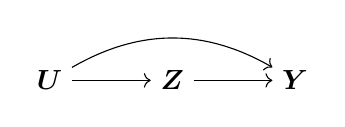
\begin{tikzpicture}
\node (1) {$\bm U$};
\node[right=of 1] (2) {$\bm Z$};
\node[right=of 2] (3) {$\bm Y$};
\draw[->] (1) to (2);
\draw[->] (1) to [out=30,in=150] (3);
\draw[->] (2) to (3);
\end{tikzpicture}
}
\caption{Causal graph at the pair level.}
\label{fig:dag_compact}
\end{figure}

We first discuss some basics from causal graph theory. In a causal directed acyclic graph (DAG), nodes represent random variables, and they are connected with arrows. 
An arrow indicates potential causation from the tail variable to the head variable. No arrow signifies the absence of a causal relationship, but the presence of an arrow doesn't guarantee the occurrence of the depicted relationship. A DAG for the pair spatial data is shown in \cref{fig:dag_compact}. A backdoor path from $\bm Z$ to $\bm Y$ starts with an arrow pointing into $\bm Z$ and ends with an arrow pointing into $\bm Y$. If the path is open, conditioning on a variable on this path blocks it, and if all backdoor paths from $\bm Z$ to $\bm Y$ are blocked, the variables are called d-separated, and they are conditionally independent. 
Colliders are nodes where arrows on either side converge. These nodes block paths when left unconditioned; however, conditioning on a collider opens the path.
Since $\bm U$ blocks the backdoor path from $\bm Z$ to $\bm Y$, the conditional independence statement in \cref{ass:paired_ignorability} holds.
%
% CUT GRAPHICAL MODELS:
%
% The graphical model associated with the DAG in \cref{fig:dag_compact} specifies that the pair-level data have joint density $f(\bm u, \bm z, \bm y) = f(\bm u) f(\bm z \mid \bm u) f(\bm y \mid \bm z, \bm u)$.

The graph in \cref{fig:dag_compact} compacts the variables at the pair-level which masks the underlying dependencies that are important for investigating identifiability of causal contrasts with unit-level analyses in spatial scenarios. The two units are depicted separately in \cref{fig:dag_expanded}.
The scenarios we consider in this manuscript are depicted in \cref{fig:dag_expanded_considered}: we do not delve into the situation where the outcome is inherently spatial ($Y_1, \leftrightarrow Y_2$ missing), or the case where $U$ in one location predicts $Z$ in a different location.
%
The double-headed arrows between $U_1, U_2$ and between $Z_1, Z_2$ represent {\it inherent spatial statistical dependencies} due to an underlying common trend that drives both variables.
% Inherent spatial dependence implies that the random variable is correlated across locations, the value at one location is {\it not} causally driven by the value in other locations, and this dependence cannot be directly explained by conditioning on measured covariates.
A DAG that represents this structure is shown in \cref{fig:dag_underlying}: $U^u$ induces correlation between $U_1$ and $U_2$, and similarly for $Z^u, Z_1$, and $Z_2.$ 
%
% CUT GRAPHICAL MODELS
%
%Therefore, the graphical model associated with the graph in \cref{fig:dag_expanded_considered} is the graphical model for the DAG in \cref{fig:dag_underlying}, and \( f(u^u, \bm u, z^u, \bm z, \bm y) \) can be written as
% { \(
% f(u^u) f(u_1 \mid u^u) f(u_2 \mid u^u) f(z^u) f(z_1 \mid z^u, u_1) f(z_2 \mid z^u, z_2)
% f(y_1 \mid z_1, z_2, u_1, u_2) f(y_2 \mid z_2, z_1, u_2, u_1).
% \)}
The superscript $^u$ is used to stand for {\it u}nderlying variables that drive the spatial structure in the corresponding variable.
% As an example, a vector $\bm Z = (Z_1, Z_2)$ that follows a bivariate normal distribution with variances 1 and correlation parameter $\rho$ can be equivalently conceived as arising from a generative process where $Z^u, \epsilon_1, \epsilon_2 \sim N(0, 1)$ independently, and $Z_i = \sqrt{\rho} Z^u + \sqrt{1 - \rho} \epsilon_i$. Here $Z^u$ drives the underlying common trend in $\bm Z$, but $Z^u$ is unobserv\textit{able}, and it can {\it never} be measured or conditioned on. 
Such inherent spatial dependence in the treatment variable can occur, for example, by experimental design if different restrictions are applied (or resources are provided) to different geographical areas which would lead to spatially correlated treatment assignments.
Inherent spatial structure can also arise by exogenous processes that are possible to measure {\it in theory} but not in practice, such as the intricate atmospheric and pollution transport processes that dictate the spatially-correlated ambient air pollution levels.
Therefore, the underlying $U^u$ and $Z^u$ describe the inherent spatial structure in $\bm U$ and $\bm Z$ which cannot be ``adjusted away'' by conditioning on more covariates.
Finally, the term {\it spatial confounding} is used to represent the situation where an inherently spatial variable ($U_1 \leftrightarrow U_2$) confounds the relationship of interest, in that it leads to open backdoor paths from the treatment to the outcome.

\begin{figure}[!t]
\spacingset{1.25}
\vspace{-40pt}
\begin{subfigure}[t]{.3\linewidth}
\centering
\resizebox{\textwidth}{!}{
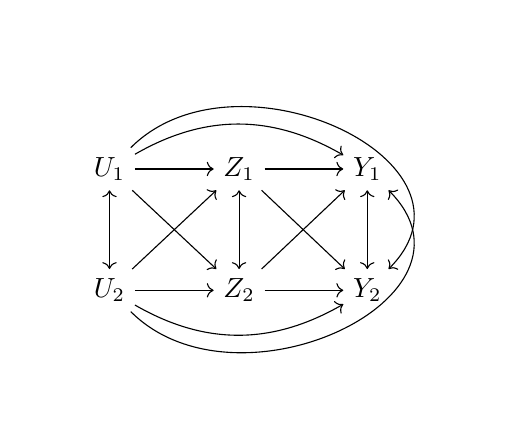
\begin{tikzpicture}
        \node (1) {$U_1$};
		\node[ right= of 1] (2) {$Z_1$};
		\node[ right= of 2] (3) {$Y_1$};
		\node[below = of 1] (12) {$U_2$};
		\node[ right= of 12] (22) {$Z_2$};
		\node[ right= of 22] (32) {$Y_2$};
		\draw[->] (1) to (2); 
		\draw[->] (12) to (2); 
		\draw[->] (1) to (22); 
		\draw[->] (12) to (22); 
		\draw[->] (2) to (3); 
		\draw[->] (2) to (32);
		\draw[->] (22) to (3);
		\draw[->] (12) to [out=330,in=210] (32);
		\draw[->] (1) to [out=45,in=45,looseness=1.35] (32);
\phantom{\draw[->] (32) to [out=60,in=120,looseness=1.15] (1);}
%\phantom{\node [below left =0.25 and 0.25 of 1] (10) {$U$};}
		\draw[->] (12) to [out=315,in=315,looseness=1.35] (3);
		\draw[->] (1) to [out=30,in=150] (3);
		\draw[->] (22) to (32);
		\draw[<->] (1) to (12);
		\draw[<->] (2) to (22);
		\draw[<->] (3) to (32);
	\end{tikzpicture}
}
\vspace{-35pt}
\caption{The two units depicted separately with all possible causal and statistical relationships.}
\label{fig:dag_expanded}
\end{subfigure}
%
\hfill
\begin{subfigure}[t]{.3\linewidth}
\centering
\resizebox{\textwidth}{!}{
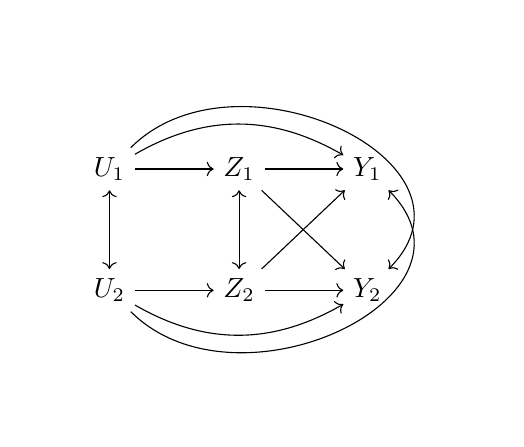
\begin{tikzpicture}
        \node (1) {$U_1$};
		\node[ right= of 1] (2) {$Z_1$};
		\node[ right= of 2] (3) {$Y_1$};
		\node[below = of 1] (12) {$U_2$};
		\node[ right= of 12] (22) {$Z_2$};
		\node[ right= of 22] (32) {$Y_2$};
		\draw[->] (1) to (2); 
		\draw[->] (12) to (22); 
		\draw[->] (2) to (3); 
		\draw[->] (2) to (32);
		\draw[->] (22) to (3);
		\draw[->] (12) to [out=330,in=210] (32);
		\draw[->] (1) to [out=45,in=45,looseness=1.35] (32);
\phantom{\draw[->] (32) to [out=60,in=120,looseness=1.15] (1);}
		\draw[->] (12) to [out=315,in=315,looseness=1.35] (3);
		\draw[->] (1) to [out=30,in=150] (3);
		\draw[->] (22) to (32);
		\draw[<->] (1) to (12);
		\draw[<->] (2) to (22);
	\end{tikzpicture}
}
\vspace{-35pt}
\caption{The two units with the relationships we consider in this work.}
\label{fig:dag_expanded_considered}
\end{subfigure}
\hfill
\begin{subfigure}[t]{.32\linewidth}
\centering
\resizebox{\textwidth}{!}{
\begin{tikzpicture}
        \node (1) {$U_1$};
        \node [below left =0.25 and 0.25 of 1] (10) {$U^u$};
        \node [below left =0.25 and 0.25 of 2] (20) {$Z^u$};
		\node[ right= of 1] (2) {$Z_1$};
		\node[ right= of 2] (3) {$Y_1$};
		\node[below = of 1] (12) {$U_2$};
		\node[ right= of 12] (22) {$Z_2$};
		\node[ right= of 22] (32) {$Y_2$};
		\draw[->] (1) to (2); 
		\draw[->] (12) to (22); 
		\draw[->] (2) to (3); 
		\draw[->] (2) to (32);
		\draw[->] (22) to (3);
		\draw[->] (12) to [out=330,in=210] (32);
		\draw[->] (1) to [out=45,in=45,looseness=1.35] (32);
		\draw[->] (12) to [out=315,in=315,looseness=1.35] (3);
		\draw[->] (1) to [out=30,in=150] (3);
		\draw[->] (22) to (32);
		\draw[->] (10) to (1);
		\draw[->] (10) to (12); 
		\draw[->] (20) to (2);
		\draw[->] (20) to (22);
\end{tikzpicture}
}
\vspace{-35pt}
\caption{Statistical dependencies occur due to an unobservable underlying common trend.}
\label{fig:dag_underlying}
\end{subfigure}
\vspace{-5pt}
\caption{Pair-level causal and statistical dependencies depicted at the unit-level. 
% CUT!!!
%(a) Compacted across units. (b) The two units in the pair are depicted separately with all possible relationships allowed. (c) Subgraph we consider in this manuscript with some arrows missing. (d) Statistical dependencies are conceived as occurring due an underlying unobservable trend component. 
}
\label{fig:dag}
\end{figure}


In \cref{fig:graphs} we present causal diagrams with spatial confounding, interference, and inherent spatial dependence that correspond to subgraphs of \cref{fig:dag_expanded_considered} with different arrows missing. A researcher that is interested in drawing causal inferences does not know which of these graphs describes the dependencies in their data. We use these graphs to illustrate the complications and biases in estimating causal effects from unit-level analyses that manifest {\it due to} the spatial dependence in the covariate and the treatment.
Conditional independence and identifiability statements are based on viewing the inherent spatial dependencies within the realm of the underlying DAG in \cref{fig:dag_underlying}.
All the identifiability results discussed in this section 
are stated and proven in Supplement \ref{supp_sec:identifiability}, some of which are based on well-known theory of graphical models \citep{spirtes1993causation, pearl1995causal, pearl2000models}.


The graphs in Figures \ref{fig:direct} and \ref{fig:general_spatial_conf} correspond to scenarios with spatial confounding and no interference.
Scenario \ref{fig:direct} represents the case of {\it direct} spatial confounding where it is only the {\it local} value of $U$ that drives the local value for $Y$. In this scenario there exists {\it statistical}, but no {\it causal}, dependence across units.
Scenario \ref{fig:general_spatial_conf} allows also for {\it indirect} spatial confounding, which describes a causal dependence across units in that a local spatial predictor of the exposure ($U_j \rightarrow Z_j$) predicts the outcome in a different location ($U_j \rightarrow Y_i$).

Under scenario \ref{fig:direct}, to identify the local causal effects it suffices to control for the local value of the confounder.
However, there are four backdoor paths for the interference effect of Unit 2's treatment on Unit 1's outcome, $\iota_1(z)$:
\begin{enumerate*}[label=(\Alph*)]
\item $Z_2 \leftarrow U_2 \leftrightarrow U_1 \rightarrow Y_1$,
\item $Z_2 \leftarrow U_2 \leftrightarrow U_1 \rightarrow Z_1 \rightarrow Y_1$,
\item $Z_2 \leftrightarrow Z_1 \leftarrow U_1 \rightarrow Y_1$, and
\item $Z_2 \leftrightarrow Z_1 \rightarrow Y_1$.
\end{enumerate*}
Paths (A) and (B), and paths (C) and (D) exist because $\bm U$ and $\bm Z$ are inherently spatial, respectively. If they were {\it not} spatial and the two units were independent, the backdoor paths would not exist, and one could identify interference effects without any adjustments.
With spatial data, these same analyses would mis-attribute spatial statistical dependence to interference, and mis-identify the presence of spatial interference.
Instead, local and interference effects should be investigated simultaneously adjusting for the local value of the confounder. However, in the presence of indirect spatial confounding in Scenario \ref{fig:general_spatial_conf}, adjusting for the neighbor's exposure opens the path $Z_i \leftrightarrow Z_j \leftarrow U_j \rightarrow Y_i$ on which $Z_j$ is a collider, and breaks identifiability of the local effect. In this scenario, one needs to adjust for the local {\it and} the neighbor's confounder value in order to identify local and interference effects.
Since this path is only present when $\bm Z$ is spatial, this notion of confounding pertains solely to the setting with dependent data, and it is not met in settings with independent observations.

%Even in this simple scenario, the data's inherent spatial dependence ``breaks'' the analyses that would be valid for independent data.



%\paragraph{Direct and indirect spatial confounding without interference}

% -- comment: the point here is that in 3a we can do local + interference and it wont hurt the local estimation. Here if we do local + interfernece, it will hurt estimation of local unless we adjust for U2.

% At the same time, to identify the interference effect $\iota_i(z)$, one would need to adjust on the neighbor's confounder value $U_j$ in order to block the backdoor path $Z_j \leftarrow U_j \rightarrow Y_i$.
% The spatial confounder in location $j$, $U_j$, is not a confounder of the local causal effect at location $i$, $\lambda_i(z)$, in the classic sense since it is not a predictor of the exposure at location $i$ (missing arrow from $U_j$ to $Z_i$). Instead, $U_j$ indirectly confounds the $(Z_i, Y_i)$ relationship due to the $Z_i - Z_j \leftarrow U_j \rightarrow Y_i$ path.
% Indirect confounding can occur even if direct confounding does not exist, if for example the local predictor of the exposure is not a predictor of the local outcome ($U_i \rightarrow Z_i$, $U_i \rightarrow Y_j$, but $U_i \not\rightarrow Y_i$).



\begin{figure}[!t]
\spacingset{1.1}
\centering
\small
\vspace{-10pt}
% DIRECT SPATIAL CONFOUNDING
\begin{subfigure}[t]{.3\linewidth}
\centering
\resizebox{.9\linewidth}{!}{
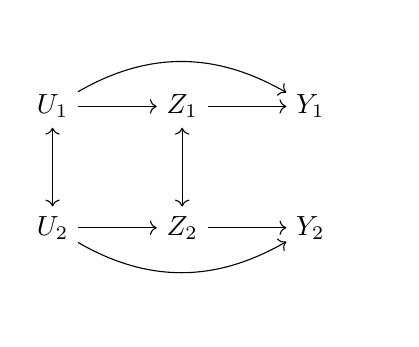
\begin{tikzpicture}
		\node (1) {$U_1$};
		\node[ right= of 1] (2) {$Z_1$};
		\node[ right= of 2] (3) {$Y_1$};
		\node[below = of 1] (12) {$U_2$};
		\node[ right= of 12] (22) {$Z_2$};
		\node[ right= of 22] (32) {$Y_2$};
		\draw[->] (1) to (2);
		\draw[->] (1) to [out=30,in=150] (3);
		\draw[->] (2) to (3); 
		\draw[->] (12) to (22);
		\draw[->] (12) to [out=330,in=210] (32);
		\draw[->] (22) to (32);
		\draw[<->] (1) to (12);
		\draw[<->] (2) to (22);
            \phantom{
		\clip (0,-2.7) rectangle (4.3,1);
		\draw[->] (1) to [out=45,in=45,looseness=1.35] (32);
		\draw[->] (12) to [out=315,in=315,looseness=1.35] (3);
		}
	\end{tikzpicture}
 }
 \vspace{-5pt}
\caption{{\bf Direct Spatial Confounding.}
The covariate predicts the exposure and the outcome only locally. 
% CUT!!!
%Adjusting for the confounder is necessary for identifying both local and interference effects.
}
\label{fig:direct}
\end{subfigure}
\hfill
%
% DIRECT AND INDIRECT SPATIAL CONFOUNDING
\begin{subfigure}[t]{.3\linewidth}
\centering
\resizebox{.9\linewidth}{!}{
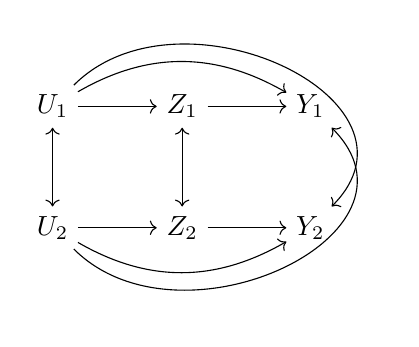
\begin{tikzpicture}
		\node (1) {$U_1$};
		\node[ right= of 1] (2) {$Z_1$};
		\node[ right= of 2] (3) {$Y_1$};
		\node[below = of 1] (12) {$U_2$};
		\node[ right= of 12] (22) {$Z_2$};
		\node[ right= of 22] (32) {$Y_2$};
		\draw[->] (1) to (2);
		\draw[->] (1) to [out=30,in=150] (3);
		\draw[->] (2) to (3); 
		\draw[->] (12) to (22);
		\draw[->] (12) to [out=330,in=210] (32);
		\draw[->] (22) to (32);
		\draw[<->] (1) to (12);
		\draw[<->] (2) to (22);
	    \clip (0,-2.7) rectangle (4.3,1);
		\draw[->] (1) to [out=45,in=45,looseness=1.35] (32);
		\draw[->] (12) to [out=315,in=315,looseness=1.35] (3);
	\end{tikzpicture}
} \vspace{-5pt}
\caption{{\bf Direct \& Indirect Spatial Confounding.}
The covariate predicts the local and neighbor's outcome.
% CUT!!!
%Local and neighbor's covariate has to be adjusted for identifying local and interference effects.
}
\label{fig:general_spatial_conf}
\end{subfigure}
\hfill
%
% INTERFERENCE
\begin{subfigure}[t]{.3\linewidth}
\centering
\resizebox{.9\linewidth}{!}{
\begin{tikzpicture}
		\node (1) {$U_1$};
		\node[ right= of 1] (2) {$Z_1$};
		\node[ right= of 2] (3) {$Y_1$};
		\node[below = of 1] (12) {$U_2$};
		\node[ right= of 12] (22) {$Z_2$};
		\node[ right= of 22] (32) {$Y_2$};
		\draw[->] (2) to (3); 
		\draw[->] (2) to (32);
		\draw[->] (22) to (3);
		\phantom{\draw[->] (12) to [out=330,in=210] (32);}
		\draw[->] (22) to (32);
		\draw[<->] (1) to (12);
		\draw[<->] (2) to (22);
             \phantom{
		\clip (0,-2.7) rectangle (4.3,1);
		\draw[->] (1) to [out=45,in=45,looseness=1.35] (32);
		\draw[->] (12) to [out=315,in=315,looseness=1.35] (3);
		}
	\end{tikzpicture}
 }
 \vspace{-5pt}
\caption{{\bf Spatial interference.}
One unit's treatment affects the other unit's outcome.
Spatial covariates are not confounders.}
\label{fig:interference}
\end{subfigure}
%
$\ $ \\[-2pt]
%
% INTERFERENCE ONLY
\begin{subfigure}[t]{.3\linewidth}
\centering
\resizebox{.9\linewidth}{!}{
\begin{tikzpicture}
		\node (1) {$U_1$};
		\node[ right= of 1] (2) {$Z_1$};
		\node[ right= of 2] (3) {$Y_1$};
		\node[below = of 1] (12) {$U_2$};
		\node[ right= of 12] (22) {$Z_2$};
		\node[ right= of 22] (32) {$Y_2$};
		\draw[->] (1) to (2);
		\draw[->] (2) to (32);
		\draw[->] (22) to (3);
		\draw[->] (2) to (3); 
		\draw[->] (12) to (22);
		\draw[->] (22) to (32);
		\draw[<->] (1) to (12);
		\draw[<->] (2) to (22);
		\phantom{
		\clip (0,-2.7) rectangle (4.3,1);
		\draw[->] (1) to [out=45,in=45,looseness=1.35] (32);
		\draw[->] (12) to [out=315,in=315,looseness=1.35] (3);
		}
	\end{tikzpicture}
}
\vspace{-5pt}
\caption{{\bf Interference and a spatial predictor of the exposure.}
% CUT!!!
% If interference is not accounted for, methods that adjust and do not adjust for unmeasured spatial variables will return different estimates, both of which are wrong. Therefore, unaccounted interference would manifest as spatial confounding.
}
\label{fig:predictor_interference}
\end{subfigure}
\hfill
%
% DIRECT SPATIAL CONFOUNDING AND INTERFERENCE
\begin{subfigure}[t]{.3\linewidth}
\centering
\resizebox{.9\linewidth}{!}{
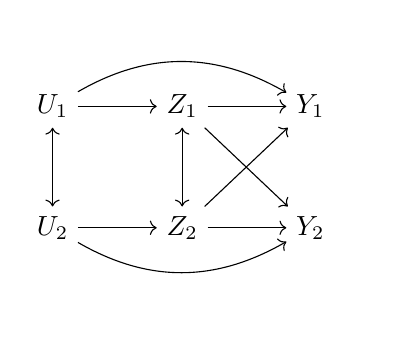
\begin{tikzpicture}
		\node (1) {$U_1$};
		\node[ right= of 1] (2) {$Z_1$};
		\node[ right= of 2] (3) {$Y_1$};
		\node[below = of 1] (12) {$U_2$};
		\node[ right= of 12] (22) {$Z_2$};
		\node[ right= of 22] (32) {$Y_2$};
		\draw[->] (1) to (2);
		\draw[->] (2) to (32);
		\draw[->] (22) to (3);
		\draw[->] (1) to [out=30,in=150] (3);
		\draw[->] (2) to (3); 
		\draw[->] (12) to (22);
		\draw[->] (12) to [out=330,in=210] (32);
		\draw[->] (22) to (32);
		\draw[<->] (1) to (12);
		\draw[<->] (2) to (22);
		\phantom{
		\clip (0,-2.7) rectangle (4.3,1);
		\draw[->] (1) to [out=45,in=45,looseness=1.35] (32);
		\draw[->] (12) to [out=315,in=315,looseness=1.35] (3);
		}
	\end{tikzpicture}
 }
 \vspace{-5pt}
\caption{{\bf Direct Spatial Confounding and Interference.} 
% CUT!!!
% Conditioning on both exposure values and the local confounder is necessary for identifying local and interference effects due to the inherent spatial structure in $\bm U$ and $\bm Z$. 
}
\label{fig:direct_interference}
\end{subfigure}
\hfill
%
% ALL SPATIAL CONFOUNDING AND INTERFERENCE
\begin{subfigure}[t]{.32\linewidth}
\centering
\resizebox{.9\linewidth}{!}{
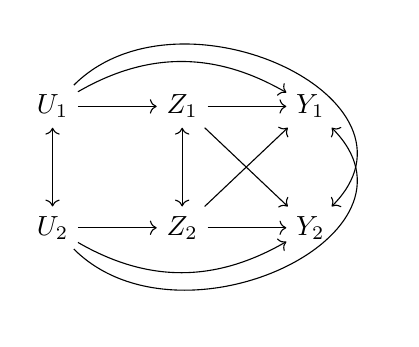
\begin{tikzpicture}
		\node (1) {$U_1$};
		\node[ right= of 1] (2) {$Z_1$};
		\node[ right= of 2] (3) {$Y_1$};
		\node[below = of 1] (12) {$U_2$};
		\node[ right= of 12] (22) {$Z_2$};
		\node[ right= of 22] (32) {$Y_2$};
		\draw[->] (1) to (2);
		\draw[->] (1) to [out=30,in=150] (3);
		\draw[->] (2) to (3); 
		\draw[->] (12) to (22);
		\draw[->] (12) to [out=330,in=210] (32);
		\draw[->] (22) to (32);
		\draw[->] (2) to (32);
		\draw[->] (22) to (3);
		\draw[<->] (1) to (12);
		\draw[<->] (2) to (22);
	    \clip (0,-2.7) rectangle (4.3,1);
		\draw[->] (1) to [out=45,in=45,looseness=1.35] (32);
		\draw[->] (12) to [out=315,in=315,looseness=1.35] (3);
	\end{tikzpicture}
}
\vspace{-5pt}
\caption{{\bf Direct, Indirect Spatial Confounding, and Interference.} The complete graph we consider. 
%CUT!!!
%Local and interference effects should be investigated simultaneously while also conditioning on the local and neighborhood covariates.
}
\label{fig:general_interference}
\end{subfigure}
% \vspace{10pt}
\caption{Graphical representation of spatial confounding and interference with a spatially correlated covariate $\bm U = (U_1, U_2)$, a spatial exposure $\bm Z = (Z_1, Z_2)$, and outcome $\bm Y = (Y_1, Y_2)$.}
\label{fig:graphs}
\end{figure}





% \paragraph{Interference without spatial confounding}

\cref{fig:interference} represents a setting with interference and no spatial confounding. 
%where the spatial covariates are not confounders, but interference might be present because a unit's outcome can be driven by the neighbor's treatment.
If the exposure $\bm Z$ is not spatially-structured, the local effect for Unit $i$ can be identified by contrasting the average outcome for this unit among pairs with $Z_i = 1$ and pairs with $Z_i = 0$, without any adjustment. These local effects are different than the ones in \cref{sec:pairs}, though they are still interpretable (see Supplement \ref{supp_sec:identifiability}).
However, when $\bm Z$ is inherently spatial, the correlation of $Z_1, Z_2$ and the interference effect of $Z_2$ on $Y_1$ leads to spurious associations for $Z_1$ and $Y_1$, and an estimated quantity that lacks causal interpretation as a local effect.
Hence, an analysis that is valid for independent exposures is invalidated for spatially structured exposure variables, even in the complete absence of confounding variables.
A similar argument holds for the identification of interference effects for spatial and non-spatial exposures. Therefore, when the exposure is spatial, local and interference effects have to be investigated simultaneously.

In the graph of \cref{fig:predictor_interference}, the covariate, $\bm U$, is now a spatial predictor of the exposure but it is not a confounder for the local or the interference effect. For the local effect, there is one additional open backdoor path, $Z_1 \leftarrow U_1 \leftrightarrow U_2 \rightarrow Z_2 \rightarrow Y_1$, compared to the setting in \cref{fig:interference}.
A researcher might be interested in estimating local effects, while ignoring that interference might be present. Their analysis might adjust for the local variable $U$, or not. The two analyses will return different values for the local effect estimate, none of which is causally interpretable. Therefore, in this scenario, spatial interference could be mis-interpreted as spatial confounding.


%\paragraph{Direct confounding with interference}

\cref{fig:direct_interference} shows a setting with {direct spatial confounding and interference}, which combines the scenarios in Figures \ref{fig:direct} and \ref{fig:interference}. When $\bm Z$ is inherently spatial, it is necessary to condition on the local value of the confounder {\it and} the neighbor's exposure to identify local effects. In contrast, if $\bm Z$ is not inherently spatial, interpretable local effects can be identified conditioning only on the local value of the confounder (see Supplement \ref{supp_sec:identifiability}). Similar conclusions can be drawn about the identifiability of interference effects. We again see that the exposure's inherent spatial structure can lead to misleading conclusions if not properly accommodated.

%In the case of a spatial exposure ($Z_1-Z_2$), conditioning on the predictors of the exposure alone does not suffice to identify local effects due to the spurious association between $Z_i$ and $Y_i$ that flows through $Z_j$, and the neighbors' exposure value has to be conditioned on as well. Interference effects can be identified conditional only on the local confounder and exposure values.
%In the absence of spatial correlation in the exposure ($Z_1 \leftrightarrow Z_2$ is missing), the neighbors' exposure will no longer be confounding one's exposure-outcome relationship, and local causal effects can be identified without adjustment for the neighbors' exposure.



%\paragraph{Direct and indirect confounding with interference}

Lastly, the graph in \cref{fig:general_interference} represents the situation also shown in \cref{fig:dag_expanded_considered} with direct spatial confounding, indirect spatial confounding, and interference, of which the other graphs are special cases.
%
% It is demonstrated in the figures below that if we do not adjust for the neighbors' spatial confounders, it will lead to incorrect estimates of the neighbors' exposure effect on one's outcome.


% \paragraph{}

%Particularly relevant is the work by \cite{ogburn2014causal} where they introduced causal diagrams for causal inference with interference, and use these graphs to determine identifiability of causal estimands.  They find that neighbors' covariate values often need to be controlled for in order to block all backdoor paths. This observation was also established by \cite{forastiere2021identification}, and \cite{tec2022weather2vec} developed an approach using neural networks for finding the appropriate adjustment form for the neighborhood covariates. % However, the work by \cite{ogburn2014causal} does not directly address non-causal dependencies among observations that might naturally occur in spatial settings. 
% Relatedly, \cite{vansteelandt2007confounding} considers the setting where treatments within a cluster can be correlated due to unmeasured cluster-level variables, but they do not investigate the interplay between statistical dependencies in confounders and exposures.

% The following based on:
%
%Particularly relevant is the work by \cite{ogburn2014causal} where they introduced causal diagrams for causal inference with interference, and use these graphs to determine identifiability of causal estimands.  They find that neighbors' covariate values often need to be controlled for in order to block all backdoor paths. This observation was also established by \cite{forastiere2021identification}, and \cite{tec2022weather2vec} developed an approach using neural networks for finding the appropriate adjustment form for the neighborhood covariates. % However, the work by \cite{ogburn2014causal} does not directly address non-causal dependencies among observations that might naturally occur in spatial settings. 
% Relatedly, \cite{vansteelandt2007confounding} considers the setting where treatments within a cluster can be correlated due to unmeasured cluster-level variables, but they do not investigate the interplay between statistical dependencies in confounders and exposures.
In the presence of interference, it has been previously advocated that neighbors' covariate values have to be adjusted for \citep{ogburn2014causal, forastiere2021identification}.
However, this previous work does not address non-causal dependencies among observations that might naturally occur in spatial settings. \cite{vansteelandt2007confounding} considers the setting where treatments within a cluster can be correlated due to unmeasured cluster-level variables, but they do not investigate the role of statistical dependencies in confounders and exposures.
%
% We found that when dependencies across locations are present due to missing conditioning variables, one could collect additional covariate information to ensure that data are as close to conditionally independent as possible.

We have addressed both of these points. We have illustrated that adjusting for neighbors' covariate information is particularly important for spatial data analysis.
Furthermore, in spatial settings, variables might remain dependent irrespective of how many covariates we condition on. We have established that the variables' inherent dependence structures lead to challenges in separating statistical dependencies from causal relationships, and accurately attributing causal effects. 
Our investigations illustrate that spatial settings are intrinsically different from settings with independent observations, in that confounding and causal dependencies can manifest as each other unless the spatial structure of the data is comprehensively accounted for.

These points are illustrated with a motivating simulation study in Supplement \ref{subsec:illustrate_bias_pairs}, where we illustrate biases of estimators that condition on different sets of variables. We see in practice how researchers might mis-attribute spatial confounding to interference, or mis-identify spatial confounding if interference is not accounted for. We also see that the estimators' biases increase with the strength of the variables' spatial dependence.
Importantly, across all scenarios, simultaneously estimating local and interference effects while adjusting for local and neighborhood confounder values eliminates biases due to spatial dependencies, an important practical guidance for researchers aiming to draw causal inferences from spatial data.
% Across all scenarios, adjusting for the local and neighborhood exposure and confounder value returns unbiased local and interference estimates.




\section{Causal inference with spatial dependencies on a spatial network}
\label{sec:one_network}

In the case of a spatial network of interconnected units, the population of interest cannot be partitioned in non-interacting groups, and defining and estimating causal effects is more challenging. Estimation techniques that consider blocks of interconnected units (such as the pairs of \cref{sec:pairs}) as the unit of analysis cannot be applied, and unit-level analyses are the only option. In \cref{subsec:po_network} we introduce potential outcomes for units across space based on an exposure mapping, in \cref{subsec:network_ignorability} we introduce ignorability for spatial data with unmeasured confounding, in \cref{subsec:sem_estimands} we establish estimands based on structural equation modeling, and in \cref{subsec:illustrate_bias_network} we discuss the interplay between statistical and causal dependence in spatial data.


\subsection{Potential outcomes based on network connections and exposure mapping}
\label{subsec:po_network}

Let $Z_i \in \mathcal{Z}$ denote the treatment value of unit $i = 1, 2, \dots, n$, which can be binary or continuous. Continuous treatments are often referred to as exposures, so we use the two terms interchangeably. In full generality, a unit's potential outcomes depend on the treatment level of all units on the spatial network, denoted by $Y_i(\bm z)$ for $\bm z \in \mathcal{Z}^n$. 
%By decomposing the treatment vector $\bm z$ in unit $i$'s treatment and the treatment of all others $\bm z = (z_i, \bm z_{-i})$, potential outcomes can also be denoted as $Y_i(z_i, \bm z_{-i})$.
We reduce the number of potential outcomes by assuming the presence of a known interference network and exposure mapping \citep{aronow2017estimating, zigler2020bipartite, forastiere2021identification}. Let $A$ denote a known adjacency matrix of dimension $n \times n$, where $A_{ij} = 1$ reflects that the outcome for unit $i$ might depend on unit $j$'s treatment level, $A_{ij} = 0$ otherwise, and all diagonal elements are 0.
%We set the diagonal elements, $A_{ii}$, to 0
%We use $A_{i(-i)}$ to denote the $i^{th}$ row of the matrix excluding the diagonal element, therefore reflecting unit $i$'s connections.
We assume that unit $i$'s potential outcomes depend on the treatment vector only through its own exposure, and the average exposure of units with which it is connected through $A$:

\begin{assumption}
% Let $g:\mathcal{Z}^{n - 1} \times \{0, 1\}^{n - 1} \rightarrow \mathcal{E}$ denote a known function that maps the treatment vector and vector of connections for $n - 1$ units to an exposure value in $\mathcal{E}$.
Let $\bm z, \bm z'$ be two treatment vectors in $\mathcal{Z}^n$ such that $z_i = z_i'$ and $\overline z_i = \overline z_i'$, where $\overline z_i = \sum_j A_{ij} z_j / \sum_j A_{ij},$ and similarly for $\overline z_i'$. It holds that $Y_i(\bm z) = Y_i(\bm z')$, and the potential outcome $Y_i(\bm z)$ can be denoted as $Y_i(z_i, \overline z_i).$
\label{ass:sutva}
\end{assumption}

For areal data, a binary adjacency matrix $A$ often makes sense. However, for the case of point-referenced data the adjacency matrix could be defined as a function of the units' geographical distance with zero-elements on the diagonal. Then, the average neighborhood exposure in \cref{ass:sutva} would be a weighted average of the exposures of other locations, with weights driven by the locations' geographic proximity. In settings of spatial interference, exposure mappings have been previously defined based on atmospheric processes in \cite{zigler2020bipartite}, and on population mobility in \cite{shin2023spatial}.
Our discussion below would straightforwardly accommodate an asymmetric, weighted adjacency matrix $A$, or a definition of exposure mapping that is more intricate than the average neighborhood exposure in \cref{ass:sutva}. % We maintain these here for simplicity.


\subsection{Ignorability in terms of measured and unmeasured spatial covariates}
\label{subsec:network_ignorability}

For identifying and estimating causal effects from observational data, a set of covariates that satisfies ignorability has to be conditioned on. If unconfoundedness is not satisfied based on measured covariates, biases for estimating causal effects persist. For the $n$ units in the network, let $\widetilde C_i = (C_{i1}, C_{i2}, \dots, C_{ip})^T$ denote unit $i$'s $p$ measured covariates, which include individual and neighborhood characteristics. However, these covariates are not a sufficient conditioning set for unconfoundedness of the treatment assignment, and 
\begin{equation}
(Z_i, \overline Z_i) \not\!\indep Y_i(z, \overline z) \mid \widetilde C_i.
\label{eq:not_ignorable}
\end{equation}
We assume however that ignorability holds conditional on measured covariates, and the local and neighborhood value of an unmeasured covariate.
\begin{assumption}
%[Ignorability conditional on unmeasured local and neighborhood covariate]
There exists unmeasured covariate $\bm U = (U_1, U_2, \dots, U_n)$ such that
\( \displaystyle
(Z_i, \overline Z_i) \indep Y_i(z, \overline z) \mid \widetilde C_i, U_i, \overline U_i,
\)
for all $z, \overline z$, where $\overline U_i$ is the average value of $U$ in the neighborhood of $i$, $\overline U_i = \sum_j A_{ij}U_j / \sum_j A_{ij}$.
Also, it holds that $f(Z_i = z, \overline Z_i = \overline z_i \mid \widetilde C_i, U_i, \overline U_i) > 0$.
\label{ass:network_ignorability}
\end{assumption}
%
\cref{ass:network_ignorability} resembles the unconfoundedness assumption on the individual and neighborhood treatment for network data in \cite{forastiere2021identification} and \cite{ zigler2020bipartite}, though here we allow for confounding from local and neighborhood values of an unmeasured covariate.


\subsection{Local and interference effects within a structural equation framework}
\label{subsec:sem_estimands}

We discuss estimands of interest within the realm of a structural equation model. We assume that for functions $f_1, f_2, f_3$, the potential outcomes arise according to
\begin{equation}
Y_i(z, \overline z) = f_1(z, \overline z) + f_2(\widetilde C_i) + f_3(U_i, \overline U_i) + \epsilon_i(z, \overline z)
\label{eq:sem}
\end{equation}
where $\epsilon_i(z, \overline z)$ are independent mean zero random variables with variance $\sigma^2_Y$. The independence of the error terms across units is a structural representation of the absence of outcome dependence in the graphs of \cref{fig:graphs} (missing $Y_1 \leftrightarrow Y_2$). For $f_1, f_2, f_3$ linear, \cref{eq:sem} reduces to
\begin{equation}
Y_i(z, \overline z) = \beta_0 + \beta_Z z + \beta_{\bar Z} \overline z + \widetilde C_i^T \bm \beta_C + \beta_U U_i + \beta_{\bar U} \overline U_i + \epsilon(z, \overline z).
\label{eq:linear_sem}
\end{equation}
Then, $\beta_Z$ and $\beta_{\bar Z}$ describe the local and interference effects of the exposure, respectively, with $\beta_Z$ representing the expected change in a unit's outcome for a unit increase in its own exposure when the neighborhood exposure remains fixed, and $\beta_{\bar Z}$ representing the expected change in a unit's outcome for a unit increase in its neighborhood exposure when its individual exposure remains fixed. 
Non-linear functions and interaction terms between the local exposure, the neighborhood exposure, and the covariates  could be straightforwardly incorporated without any complications.

Structural equation models have been previously employed for defining causal estimands in spatial settings with unmeasured confounders \citep{schnell2020mitigating, christiansen2022toward, papadogeorgou2022discussion}, interference \citep{giffin2022generalized}, or both \citep{giffin2021instrumental}, though model-free definitions using potential outcomes directly have also been employed \citep[e.g.][]{Verbitsky-savitz2012, gilbert2021causal}.

The potential outcomes, ignorability assumption, and estimands introduced for data on a spatial network are in-line with the ones for paired data in \cref{sec:pairs}. By setting $A$ to be a blocked diagonal matrix with blocks of size two, the potential outcomes $Y_i(z_i, \overline z_i)$ reduce to $Y_i(z_i, z_j)$, the ignorability \cref{ass:network_ignorability} reduces to the ignorability \cref{ass:paired_ignorability}, and the estimands of interest agree, $\beta_Z = \lambda_i(z)$ and $\beta_{\bar Z} = \iota_i(z)$.
Therefore, the method in \cref{sec:method} applies both to a spatial network and pair data, with the appropriate definition of the adjacency matrix $A$.


\subsection{
%Confounding, interference and inherent spatial dependence induced bias in networks
The bias induced by spatial dependence in network data
}
\label{subsec:illustrate_bias_network}

We provide an example of how the variables' inherent spatial structure might occur in a spatial setting. This is merely an illustration, and it is not required below. We return to viewing the inherent spatial structure in $\bm U$ as driven from an underlying covariate $U^u$ as in \cref{fig:dag_underlying}. For $U^u = (U_1^u, U_2^u, \dots, U_n^u)$ vector of independent random variables, set $U_i = \sum_{j = 1}^n w_{ij} U_j^u + \epsilon_{i}$, for $w_{ij}$ not all zero and $\epsilon_i$ independent errors. Then the elements of $\bm U$ that share elements of $U^u$ are statistically dependent. If the weights $w_{ij}$ are based on the spatial proximity of $i$ and $j$, this dependence structure will be {\it spatially} driven. We can similarly conceive $Z^u$ and $\bm Z$.

Whether the coefficients in \cref{eq:linear_sem} are zero or not can be conceived in the same manner as to whether the corresponding arrows are missing or not in the graphs of \cref{fig:graphs}. 
% CUT!!! 
%For example, the structural model for $\beta_{\bar Z} = \beta_{\bar U} = 0$ is consistent with a graph resembling that in \cref{fig:direct}. 
Under the different scenarios of \cref{fig:graphs}, the ignorability \cref{ass:network_ignorability} might also hold conditional on $\widetilde C$ only, conditional on $\widetilde C$ and $U$, or might only hold conditional on all of $\widetilde C, U$ and $\overline U$.
%
In Supplement \ref{supp_sec:motivating_one_network}, we investigate the influence of spatial dependencies in learning local and interference effects from a single interconnected network of spatial data. The conclusions are the same as the ones for paired data: \begin{enumerate*}[label=(\alph*)]
\item spatial confounding and interference can manifest as each other, 
\item inherent spatial dependencies complicate standard estimation strategies and can render them invalid even in simple settings, 
\item controlling for local and neighborhood covariates is crucial for adjusting for confounding and estimating causal effects unbiasedly, and 
\item local and interference effects should be investigated simultaneoulsy in the presence of spatial dependencies.
\end{enumerate*}



\section{Bayesian inference of local and interference effects with spatial dependencies and unmeasured spatial confounding}
\label{sec:method}

Until now we have focused on the complications of identifying causal quantities in spatial settings with confounding, interference, and inherent spatial structure. When the measured covariates do not suffice for confounding adjustment, biases in effect estimation will persist.
In what follows, we develop a Bayesian approach for estimating causal effects with spatially dependent data that addresses these complications and mitigates bias due to local and neighborhood unmeasured spatial confounding. 
% CUT!!!
% Even if the unmeasured covariate is spatial, including a spatial random effect in the outcome regression will not necessarily reduce bias from unmeasured confounders \citep{schnell2020mitigating, reich2021review}.
In \cref{subsec:bayesian_treatment}, we show that, in the presence of missing confounders, it is necessary to incorporate the treatment assignment mechanism in a Bayesian causal inference procedure.
%By viewing the inherent spatial structure in the confounder and the exposure as underlying, unobservable covariates as in \cref{fig:dag_underlying}, we investigate the impact of spatial structure and unmeasured confounding within the Bayesian framework for causal inference.
These derivations inform us of the assumptions on the relationship between the unmeasured confounder and the exposure described in \cref{subsec:UZ_assumptions}. 
In \cref{subsec:identifiability}, we show theoretically that all model parameters are identifiable from data, even in the presence of unmeasured spatial confounders.
In \cref{subsec:priors}, we design sensible prior distributions for the hyperparameters of the spatial confounder by studying the implications that prior choice on hyperparameters has on the implied prior beliefs of the unmeasured covariate's confounding strength.



\subsection{The role of the treatment assignment mechanism in spatial settings}
\label{subsec:bayesian_treatment}


Bayesian causal inference views unobserved potential outcomes as missing data, and inference on causal effects is acquired from their posterior distribution \citep{rubin1978bayesian, imbens1997bayesian, ding2018causal, li2022bayesian}.
Let $\bm Z = (Z_1, Z_2, \dots, Z_n)$ denote the vector of realized exposures, $\overline{\bm Z} = (\overline Z_1, \overline Z_2, \dots, \overline Z_n)$ the vector of neighborhood exposures, $\bm C = (\widetilde C_1, \widetilde C_2, \dots, \widetilde C_n)$ the $n \times p$ matrix of measured covariates, $Y_i (\cdot)$ the collection of all potential outcomes for unit $i$, and
$\bm Y(\cdot)  = \{Y_i (\cdot), \text{ for all } i \} $ the collection of all potential outcomes for all units.
Let also $\bm Y(\cdot) = \{ \bm Y, \bm Y^{\text{miss}} \}$ where  $\bm Y = (Y_1, Y_2, \dots, Y_n)$ are the observed outcomes and $\bm Y^{\text{miss}}$ is the collection of {\it un}observed potential outcomes.
% Here, it is helpful to return to \cref{fig:dag_underlying}, and think of the spatial structure in $\bm U, \bm Z$ as driven by underlying variables $U, Z$ that are unobservable. Therefore, all inherent spatial dependent in $\bm U, \bm Z$ is captured by $U, Z$. Conditional on $U, Z$ we assume unit-exchangeability \citep{de1937foresight}, which allows us to write
% \begin{align*}
% p(\bm Y(\cdot), \bm Z, \overline{\bm Z}, \bm C ) &=
% \int p(\bm Y(\cdot), \bm Z, \overline{\bm Z}, \bm C \mid U, Z) \ p(U, Z) \ \mathrm{d}U \mathrm{d}Z \\
% &= \int \prod_{i = 1}^n p(\bm Y_i(\cdot), Z_i, \overline Z_i, \widetilde C_i \mid U, Z, \theta) \ p(\theta \mid U, Z) \ \mathrm{d}\theta \ p(U, Z) \ \mathrm{d}U \mathrm{d}Z \\
% &= \int \prod_{i = 1}^n p(\bm Y_i(\cdot), Z_i, \overline Z_i, \widetilde C_i \mid U, Z, \theta) \ p(U, Z \mid \theta) \ p(\theta) \  \mathrm{d}U \mathrm{d}Z \mathrm{d}\theta
% \end{align*}
% for some vector of parameters $\theta$.
Bayesian inference proceeds by specifying
\(
p(\bm Y(\cdot), \bm Z, \overline{\bm Z}, \bm C \mid \theta)
\) 
and a prior distribution \( p(\theta) \),
and imputing missing potential outcomes from
\begin{equation}
\begin{aligned}
p(\bm Y^{\text{miss}} \mid \bm Y, \bm Z, \overline{\bm Z}, \bm C, \theta)
%\propto & \ P(\bm Y(\cdot) , \bm Z, \overline{\bm Z}, \bm C \mid \theta) \\
\propto & \ P(\bm Z, \overline{\bm Z} \mid \bm Y(\cdot), \bm C, \theta) \  P(\bm Y(\cdot) \mid \bm C, \theta) \ P(\bm C \mid \theta).
\end{aligned}
\label{eq:impute_Ymiss}
\end{equation}
If ignorability does not hold based on measured covariates only as in \cref{eq:not_ignorable},
\(
P(\bm Z, \overline{\bm Z} \mid \bm Y(\cdot), \bm C, \theta)
\neq
P(\bm Z, \overline{\bm Z} \mid \bm C, \theta)
\). 
As a result, the treatment assignment mechanism will not ``drop out'' from \cref{eq:impute_Ymiss}, and it will be informative for the imputation of missing potential outcomes \citep{mccandless2007bayesian, ricciardi2020bayesian}.
Instead, we write $p(\bm Y(\cdot), \bm Z, \overline{\bm Z}, \bm C)$ as
\begin{align*}
%\int p(\bm Y(\cdot), \bm Z, \bm C, \bm U \mid \theta^*) \ \mathrm{d}\bm U \ p(\theta^*) \ \mathrm{d}\theta^* \\
%&=
\int
p(\bm Y(\cdot) \mid \bm Z, \bm C, \bm U, \theta^*) \ 
p(\bm Z \mid \bm C, \bm U, \theta^*) \ 
p(\bm U \mid \bm C, \theta^*) \ 
p(\bm C \mid \theta^*)
\ \mathrm{d} \bm U \ p(\theta^*) \ \mathrm{d}\theta^* 
\end{align*}
where $\overline{\bm Z}$ is excluded since it is uniquely defined based on $\bm Z$, and $\theta^*$ extends $\theta$ to include parameters governing $\bm U$. 
The structural model \cref{eq:sem} implies conditional independence among the outcomes of different units which can only depend on the vector of exposures and the unmeasured covariate through the local and neighborhood values. Therefore, 
\begin{align*}
p(\bm Y(\cdot) \mid \bm Z, \bm C, \bm U, \theta) &= \prod_{i = 1}^n p(Y_i(\cdot) \mid Z_i, \overline Z_i, \widetilde C_i, U_i, \overline U_i, \theta)
= \prod_{i = 1}^n p(Y_i(\cdot) \mid \widetilde C_i, U_i, \overline U_i, \theta),
\end{align*}
where the last equality holds from \cref{ass:network_ignorability}.
Hence, we write $p(\bm Y(\cdot), \bm Z, \overline{\bm Z}, \bm C)$ as
\begin{equation}
\int \Big[ \prod_{i = 1}^n p(Y_i(\cdot) \mid \widetilde C_i, U_i, \overline U_i, \theta) \Big] \ 
p(\bm Z \mid \bm C, \bm U, \theta) \ 
p(\bm U \mid \bm C, \theta) \ 
p(\bm C \mid \theta)
\ \mathrm{d} \bm U \ p(\theta) \ \mathrm{d}\theta.
\label{eq:bayesian_framework}
\end{equation}
Therefore, having access to $\bm U$ (in addition to $\bm C$) would in fact render the treatment assignment ignorable within the Bayesian framework.

These derivations provide interesting insights.
Since $\bm U$ is unknown, and it plays a role in the distribution of the treatment assignment in \cref{eq:bayesian_framework}, the treatment assignment has to be incorporated in a valid Bayesian procedure for imputing the missing potential outcomes. 
This establishes from a new perspective that, within the Bayesian paradigm, simply including a spatial random effect in the outcome model does \textit{not} account for unmeasured spatial confounding since incorporating an exposure model is necessary for proper inference of causal effects.

\subsection{Exposure-confounder assumptions}
\label{subsec:UZ_assumptions}

The derivations in \cref{eq:bayesian_framework} also illustrate that it is necessary to specify joint distributions on the unmeasured and measured variables in order to proceed. For continuous exposures, we consider:
\begin{assumption}
% CUT!!!
%[Joint distribution of the spatial confounder and exposure]
The unmeasured spatial confounder and the spatial exposure have a joint normal distribution conditional on the measured covariates. Specifically,
\begin{equation}
\begin{pmatrix} \bm U \\ \bm Z \end{pmatrix} \Big| \  \bm C \sim N_{2n} \left(
\begin{pmatrix} \bm 0_n \\ \gamma_0 \bm 1_n + \bm C^T \bm \gamma_C \end{pmatrix} ,
\begin{pmatrix} G & Q \\ Q^\top & H \end{pmatrix}^{-1}
\right),
\label{eq:UZ_normal}
\end{equation}
for $\bm \gamma_C$ vector of length $p$, and $G, H$ positive definite matrices. The matrix $Q$ is diagonal with elements $q_i = - \rho \sqrt{g_{ii}h_{ii}}$, where $g_{ii}, h_{ii}$ are the diagonal elements of $G, H$, respectively.
\label{ass:UZ_normal}
\end{assumption}
\noindent

The joint distribution of $\bm U, \bm Z$ is parameterized through its precision matrix. Zero elements of the precision matrix specify conditional independence of the corresponding variables. Therefore, a diagonal $Q$ encodes that $Z_i \indep \bm U_{-i} \mid U_i, \bm Z_{-i}, \bm C$, where 
$\bm U_{-i} = (U_1, \dots, U_{i-1}, U_{i + 1}, \dots, U_n)$ includes all the entries in $\bm U$ except the one for unit $i$, and $\bm Z_{-i}$ is defined similarly.
Under this light, the assumption that $Q$ is diagonal is merely a statistical representation of the absence of an arrow from $U_i$ to $Z_j$ in the graphs of Figures \ref{fig:dag} and \ref{fig:graphs}, describing that the unmeasured variable is a driver of only the local exposure level.
% \cref{ass:UZ_normal} further specifies that the conditional correlation among the local confounder and exposure value is constant across locations.
Even though $\bm U$ does not depend on $\bm C$ in \cref{ass:UZ_normal}, it is reasonable to do so, since the part of the unmeasured variable that is correlated with measured covariates is already adjusted for.

The joint distribution in \cref{ass:UZ_normal} has been previously adopted in a related setting \citep{schnell2020mitigating}. Our work illustrates two crucial parts with regards to this assumption. We have shown that adopting a joint distribution on $(\bm U, \bm Z)$ is necessary within the Bayesian framework 
(\cref{subsec:bayesian_treatment} and equation \cref{eq:bayesian_framework}). Moreover, we have linked the distributional \cref{ass:UZ_normal} to the causal relationship of variables viewed through the causal graph representation. Therefore, we provide new insights on the role and interpretation of this assumption through the lens of Bayesian causal inference, and establish how this statistical assumption can be altered based on different assumptions on the complex causal dependence of the two variables.


Since we only have one realization of the spatial exposure $\bm Z$, the conditional precision matrices $G$ and $H$ cannot be estimated without imposing some structure on their elements. We assume that $G$ and $H$ are known up to parameter vectors $\theta_U = (\tau_U, \phi_U)$ and $\theta_Z = (\tau_Z, \phi_Z)$, respectively.
To ease prior elicitation in \cref{subsec:priors} that is consistent for both areal and point-referenced data, we specify $G = \tau_U^2 (D - \phi_U A)$ in either case, where $D$ is the diagonal matrix with entries $d_i = \sum_j A_{ij}$. Similarly, we specify $H = \tau_Z^2 (D - \phi_Z A)$.

The network's adjacency matrix is used for defining the neighborhood exposure and covariate in Assumptions \ref{ass:sutva} and \ref{ass:network_ignorability}, and in the joint precision matrix in \cref{ass:UZ_normal}.
% CUT!!!
% Since $H$ is the {\it conditional} precision matrix of the exposure given measured covariates and the unmeasured covariate $\bm U$, it represents the {\it inherent} spatial dependence in the exposure. 
% By viewing $G$ and $H$ under this light,
However, these two structures need {\it not} be the same, and researchers could specify the same or different adjacency matrices for these two components. 
Furthermore, the functional form with which the exposure is included in the outcome model in \cref{eq:linear_sem} can differ from the one in the joint distribution of \cref{ass:UZ_normal}. Therefore, the framework can easily allow for non-continuous exposures to be considered.
%In the case of binary exposures, one can use a probit or logistic model for the spatial treatment variable and impose \cref{ass:UZ_normal} on the underlying linear predictor.
We illustrate these points in our data analysis in \cref{sec:application}. 


\subsection{Identifiability of model parameters in the presence of unmeasured spatial confounding}
\label{subsec:identifiability}

It is reasonable to ponder whether the model parameters are identifiable based on the observed data considering they include parameters that correspond to the unmeasured variable and its relationship with the exposure and the outcome.

First, note that the coefficients $\beta_U, \beta_{\bar U}$, and the parameter $\tau_U$ of the precision matrix $G$ are not identifiable up to scaling of the unmeasured confounder $\bm U$. To see this, consider $\bm U' = c \bm U$ for some $c \neq 0$. Then, setting $\beta_U' = \beta_U / c$, $\beta_{\bar U}' = \beta_{\bar U} / c$, and ${\tau_U^{2}}' = \tau_U^2 / c^2$ will lead to the same value of the likelihood for $(\bm Y, \bm Z, \bm U) \mid \bm C$. Therefore, without loss of generality, we set $\beta_U = 1$. Even though at first sight it might appear that we ``force'' $U$ in the outcome model by setting $\beta_U = 1$, we show in \cref{subsec:priors} that our prior for $\tau_U$ ensures that this is not the case.

The next theorem shows that, for a large enough spatial ring network, all model parameters are identifiable, including the causal effects of interest, even in the presence of unmeasured spatial confounding. The definition of a ring graph and the proof are in Supplement \ref{supp_sec:identifiability_ours}.

\begin{theorem}
Consider spatial data organized on a ring graph with $n$ nodes. Using data $(\bm Z, \bm Y)$ we can identify whether or not $\rho\phi_U = 0$. If $\rho \phi_U \neq 0$, and for $\beta_U = 1$, we have that all model parameters $(\beta_Z, \beta_{\bar Z}, \beta_{\bar U}, \rho, \tau_U, \phi_U, \tau_Z, \phi_Z, \sigma^2_Y)$
are identifiable from $(\bm Z, \bm Y)$ as $n \rightarrow \infty$.
\label{theorem:identifiability}
\end{theorem}

If $\rho \phi_U = 0$, there is no spatial predictor of the exposure and therefore no unmeasured spatial confounding. Our proof uses results from \cite{schnell2020mitigating}. However, here, we address complications that arise from the causal cross-dependence of units which impose the inclusion of the neighborhood confounder and exposure values, $\overline U$ and $\overline Z$, in the outcome model, along with additional regression coefficients and causal dependence across units. Crucially, \cref{theorem:identifiability} establishes that we can identify complex confounder structures that are not limited to local restrictions.

The proof provides interesting insights for where the information in the data comes from to identify non-local confounding structures. All spatial parameters, $(\tau_U, \phi_U, \tau_Z, \phi_Z)$, and the neighborhood confounding effects, $\beta_{\bar U}$, are identified based on the covariance structure in the exposure and the outcome residuals, and how it attenuates as a function of distance. Interestingly, neighborhood confounding effects are identified by studying the spatial structure in the outcome model residuals that is not explained by similar structure in the exposure model residuals. 

Our proof uses the ring graph assumption to acquire a closed form for the data's covariance matrix. 
Our conjecture is that identifiability holds for other spatial dependence structures that allow for a sufficient number of location pairs at different distances. This paper does not delve into a comprehensive examination of general identifiability under arbitrary spatial dependence, which is reserved for future research.


\subsection{Prior distributions for confounding adjustment}
\label{subsec:priors}

In Bayesian settings, model performance often depends on the choice of hyperparameters, and non-informative priors can lead to poor performance in certain settings \citep{gelman2008weakly}. We adopt weakly informative prior distributions for intercepts, coefficients of the measured covariates, and the local and neighborhood exposure and confounder values, the variance of the residual error in \cref{eq:linear_sem}, and the parameters of the covariance matrix in \cref{eq:UZ_normal}.

We consider measured covariates, exposure and outcome that are standardized to have mean 0 and variance 1.
We adopt independent $N(0, \sigma^2_{\text{prior}})$ prior distributions for the coefficients of all measured covariates, $\bm \beta_C, \bm \gamma_C$ and for the intercepts $\beta_0, \gamma_0$, with $\sigma^2_{\text{prior}} = 2$. 
% Next, we focus on the coefficients of the local and neighborhood confounder values, $\beta_U, \beta_{\bar U}$.
We adopt a $N(0, \sigma^2_{\text{prior},\overline U})$ prior distribution for $\beta_{\bar U},$ and we set $\sigma^2_{\text{prior},\overline U} = 0.35^2$ to express the prior belief that the importance of the neighborhood value of the confounder is smaller than that of the local value of the confounder (since $\beta_U = 1$).
For the residual variance of the outcome model in \cref{eq:linear_sem}, we specify $\sigma^2_Y \sim IG(\alpha_Y, \beta_Y)$. We follow a data-driven procedure for choosing the hyperparameters $\alpha_Y, \beta_Y$. We regress the outcome on the measured local and neighborhood exposure and the measured covariates and acquire the estimated residual variance, $\widetilde \sigma^2_Y$. 
%It is reasonable to expect that including the additional predictors $U, \overline U$ in the outcome regression should reduce the residual variance. 
We set $\alpha_Y = 3$ and $\beta_Y = 3 \ \widetilde \sigma^2_Y / 4$, which leads to a prior distribution on the residual variance that puts most of its weight on values smaller than $\widetilde \sigma^2_Y$, and specifically $P(\sigma^2_Y < \widetilde \sigma^2_Y) \approx 0.98$.

Next, we specify prior distributions for the parameters of the joint precision matrix in \cref{eq:UZ_normal}. We specify flat priors for $\phi_Z, \rho$ on the $(-1, 1)$ interval. We assume that $\phi_U > 0$, and specify $\phi_U \sim \text{Beta}(6, 6)$ to encourage values that imply some spatial dependence ($\phi_U$ away from 0) while avoiding degenerate distributions ($\phi_U$ away from 1). We also require that $\phi_Z < \phi_U$ since the exposure should vary within levels of the confounder, in line with conclusions from \cite{Paciorek2010}, \cite{schnell2020mitigating} and \cite{dupont2022spatial}.

Lastly, we decide on prior distributions for $\tau_U, \tau_Z$. The priors for these parameters can have a large effect on model performance, and their choice requires careful consideration. For simplicity we discuss in detail the situation where all nodes have the same number of neighbors, and $D = dI_n$ for some $d > 0$ and $I_n$ being the $n \times n$ identity matrix.
We can show that $\Var(U_i) \geq (d \tau_U^2)^{-1}$, where equality holds for $\rho = 0$. Since $U_i$ is a priori centered at 0, if the marginal variance of $U_i$ is small for all $i$, the vector of $\bm U$ is almost indistinguishable from the vector of all zeros, and essentially drops out from the outcome model (even though we set $\beta_U = 1$). 
% --- POTENTIAL TO DO --- % In sims can we show that U drops out when not important?
Conversely, if the marginal variance of $U_i$ is big a priori, then this prior distribution would imply a strong importance of $U$ in the outcome model (considering $\beta_U = 1$).
Therefore, our choice for the prior distribution of the hyperparameter $\tau_U$ should be informed by the implied prior distribution on the unmeasured covariate's confounding strength. We specify a prior distribution for $\tau_U$ which avoids the pathological situation that $U$ has an unrealistically high predictive accuracy for the outcome. Specifically,
we specify that $1 / \tau_U$ has a truncated mean-zero normal distribution with variance $d \sigma^2_{\text{prior}} / 2$, and truncated below at 0. 
The induced prior on $(d \tau_U^2)^{-1}$ ensures that the unmeasured variable's strength in the outcome model resembles, a priori, the measured covariates' strength in the outcome model specified by the $N(0, \sigma^2_{\text{prior}})$ prior distribution on their coefficients.

Similarly, the magnitude of $1 / (d \tau_Z^2)$ can be conceived as the variance in the exposure that cannot be explained by covariates. Therefore, $1 / \tau_Z^2$ should not be too small because we expect {\it some} inherent variability in the exposure. At the same time, it should not be too big in comparison to the residual variance of the regression of $Z$ on the measured covariates, denoted by $\widetilde \sigma^2_Z$. 
Let $\widetilde s^2_Z$ be the observed marginal variance in the exposure across locations. We specify that $1 / \tau_Z$ follows a truncated normal distribution centered at $\sqrt{d \ \widetilde \sigma^2_Z / 2}$ with standard deviation 1, truncated below at $\sqrt{d \ 0.01 \ \widetilde s^2_Z}$ and above at $\sqrt{d \ \widetilde \sigma^2_Z / 0.8}$. 

The prior distributions on $\tau_U$ and $\tau_Z$ are illustrated in Supplement \ref{supp_sec:priors}. We see that the implied prior distribution on the unmeasured variable's predictive strength allows for all reasonable values.
When the degree is not constant across nodes (which is the case in most networks), we set $d$ to be the median network degree.
We sample from the posterior distribution of model parameters using Markov chain Monte Carlo (MCMC). The algorithm is described in Supplement \ref{supp_sec:mcmc}.


\section{Simulations}
\label{sec:sims}

We perform simulations to evaluate the extent to which the approach introduced in \cref{sec:method} mitigates the bias in estimating local and interference causal effects that is caused by direct and indirect unmeasured spatial confounding and the inherent spatial dependence in the exposure.
We simulate data under the data generative mechanisms in \cref{fig:graphs}. We consider observations on a network of interconnected units represented by a line graph, where each unit is connected with two others, except for the first and last units which only have one neighbor each. 
%The exact form of the adjacency matrix for this setting is given in Supplement \ref{supp_sec:motivating_one_network}. 
Simulations with pairs of interacting observations are deferred to Supplement \ref{supp_sec:sims_pairs}.


For number of units $n \in \{200, 350, 500\}$, we generated four measured covariates from independent $N(0, 1)$ distributions, the unmeasured confounder and the exposure of interest from \cref{eq:UZ_normal}, and calculated $\overline U, \overline Z$ for each observation. The outcome was generated according to the linear model in \cref{eq:linear_sem} with $\gamma_0 = \beta_0 = 0$. The coefficients of the measured covariates were generated randomly once and were fixed to $\bm \gamma_C = (-0.35, -0.64,  0.49,  0.06)$ and $\bm \beta_C = (0.06, 0.85, 0.02, 0.33)$ throughout our simulations. We specified spatial parameters $\phi_U = 0.6, \phi_Z = 0.4,$ and $\rho = 0.35$.
For the network data, for which median node degree is equal to 2, we set $\tau^2_U = \tau^2_Z = 1$. In all cases, we set the outcome residual error variance to one. The default outcome model coefficients of the local and neighborhood exposure and unmeasured confounder were set to $\beta_Z = 1,$ $\beta_{\bar Z} = 0.8,$ $\beta_U = 1$, and $\beta_{\bar U} = 0.5$, except for when the relationship does not exist, in which case the corresponding coefficient is set to 0. These specifications match exactly the motivating simulations for the network data discussed in \cref{subsec:illustrate_bias_network} which are presented in detail in Supplement \ref{supp_sec:motivating_one_network}.

We generate 500 data sets under each of the 36 different scenarios which are combinations of the six scenarios in \cref{fig:graphs}, the three sample sizes, and for network and paired data.
We compare the proposed approach to OLS conditional on the measured covariates for estimating local and interference effects.
In the absence of unmeasured spatial confounding, the OLS estimator is most efficient for estimating causal effects since it is based on the correctly specified outcome model. Therefore, this comparison informs us of potential efficiency loss when spatial confounding is considered but it is not truly present.
In the presence of unmeasured confounding, the OLS estimator incurs confounding bias. Therefore, comparing the two approaches in this setting illuminates the extent to which our approach can alleviate this bias.
For our method, we considered two chains with 7,000 iterations as a burn-in period and thinning by 60. We report results for data sets for which the MCMC did not show signs of lack of convergence, evaluated based on the $\widehat R$ statistic \citep{vehtari2021rank} for $\beta_Z$ and $\beta_{\bar Z}$. % was at most 1.1.



\begin{table}[!b]
    \centering
\spacingset{1.25}
    \caption{Simulation results with One Interconnected Network. Bias, root mean squared error (rMSE), and coverage of 95\% intervals based on OLS and the method of \cref{sec:method}, for the local and the interference effect. We show simulation results for the 6 settings in \cref{fig:graphs}, and for sample size equal to 200, 350 and 500. Coverage rates are reported as percentages.
    }
    % \rowcolors{5}{}{gray!10}
\spacingset{1}
    \resizebox{0.95\textwidth}{!}{%
    \begin{tabular}{*{15}{c}}
        % \hline
        % \\[-10pt]
        % & & \multicolumn{13}{c}{Network data} \\[-5pt] \\
        % \cmidrule{3-15}
       & & \multicolumn{6}{c}{Local effect} & &  \multicolumn{6}{c}{Interference effect} \\
       \cmidrule(lr){3-8} \cmidrule(lr){10-15}
        \multicolumn{2}{c}{True model \&} & \multicolumn{3}{c}{OLS} &  \multicolumn{3}{c}{Our approach} &
        & \multicolumn{3}{c}{OLS} &  \multicolumn{3}{c}{Our approach} \\
        \cmidrule(lr){3-5} \cmidrule(lr){6-8} \cmidrule(lr){10-12} \cmidrule(lr){13-15}  
        \multicolumn{2}{c}{sample size} & Bias & rMSE & Cover & Bias & rMSE & Cover &
        & Bias & rMSE & Cover & Bias & rMSE & Cover \\[5pt]
    
        \hline
        \\[-10pt]
        \multirow{4}{*}{\ref{fig:direct}} & & \multicolumn{13}{c}{$\beta_{\bar Z} = 0$ and $\beta_{\bar U}=0$} \\[0pt]
        \cmidrule{7-11}
        & 200 & 0.492 & 0.505 & 0.3
        & -0.013 & 0.306 & 91.6 &
        & 0.154 & 0.186 & 72.3
        & 0.030 & 0.137 & 93.4  \\ 
        %
        & 350 & 0.499 & 0.507 & 0
        & -0.060 & 0.247 & 94.9 & 
        & 0.146 & 0.167 & 55\phantom{.0} 
        & 0.002 & 0.094 & 96.6 \\
        %
        & 500 & 0.510 & 0.516 & 0
        & -0.073 & 0.222 & 96.5 & 
        & 0.157 & 0.172 & 36\phantom{.0} 
        & 0.009 & 0.086 & 93.8 \\[3pt]
        \hline
        \\[-10pt]

         
        \multirow{4}{*}{\ref{fig:general_spatial_conf}} & &
        \multicolumn{13}{c}{$\beta_{\bar Z} = 0$}
        \\[0pt]
        \cmidrule{7-11}
        & 200 & 0.616 & 0.630 & 0 
        & -0.169 & 0.302 & 96.9 & 
        & 0.277 & 0.302 & 34.3 
        & 0.027 & 0.146 & 93.3 \\
        %
        & 350 & 0.624 & 0.632 & 0 
        & -0.188 & 0.283 & 93.5 & 
        & 0.273 & 0.288 & 15\phantom{.0} 
        & 0.004 & 0.107 & 95.7  \\
        %
        & 500 & 0.639 & 0.644 & 0 
        & -0.174 & 0.253 & 94.6 & 
        & 0.289 & 0.299 & \phantom{0}3.7 
        & 0.011 & 0.092 & 94.8 \\[3pt]
        \hline
        \\[-10pt]


        \multirow{4}{*}{\ref{fig:interference}} & &
        \multicolumn{13}{c}{$\beta_{UZ} = 0$ and $\beta_U = \beta_{\bar U} = 0$}
        \\[0pt]
        \cmidrule{7-11}
        & 200 & \phantom{-}0.003 & 0.097 & 95.3 
        & -0.027 & 0.120 & 98.8 & 
        & \phantom{-}0.004 & 0.086 & 95.7 
        & \phantom{-}0.002 & 0.087 & 96.2 \\
        %
        & 350 & -0.002 & 0.072 & 96\phantom{.0} 
        & -0.023 & 0.100 & 99.7 & 
        & -0.007 & 0.066 & 94.3 
        & -0.016 & 0.067 & 95.5 \\
        %
        & 500 & \phantom{-}0.001 & 0.067 & 92.7 
        & -0.019 & 0.094 & 98.7 & 
        & -0.001 & 0.056 & 94\phantom{.0} 
        & -0.004 & 0.059 & 94.1 \\[3pt]
        \hline
        \\[-10pt]
        
         
        \multirow{4}{*}{\ref{fig:predictor_interference}} & &
        \multicolumn{13}{c}{$\beta_U = 0$ and $\beta_{\bar U} = 0$} \\[0pt]
        \cmidrule{7-11}
        & 200 & 0.002 & 0.085 & 96\phantom{.0} 
        & -0.020 & 0.112 & 99.2 & 
        & \phantom{-}0.003 & 0.081 & 96.3 
        & \phantom{-}0.004 & 0.085 & 95.4 \\
        %
        & 350 & 0.000 & 0.064 & 95.7 
        & -0.027 & 0.125 & 96.7 & 
        & -0.006 & 0.063 & 94\phantom{.0} 
        & -0.017 & 0.068 & 93.9 \\
        %
        & 500 & 0.001 & 0.060 & 92.7 &
        -0.012 & 0.113 & 97.7 & 
        & -0.001 & 0.054 & 94\phantom{.0} 
        & -0.003 & 0.056 & 94.5 \\[3pt]
        \hline
        \\[-10pt]


        \multirow{4}{*}{\ref{fig:direct_interference}} & &
        \multicolumn{13}{c}{$\beta_{\bar U} = 0$} \\[0pt]
        \cmidrule{7-11}
        & 200 & 0.492 & 0.505 & 0.3 
        & 0.037 & 0.296 & 89.6 & 
        & 0.154 & 0.186 & 72.3 
        & \phantom{-}0.030 & 0.141 & 92\phantom{.0} \\
        %
        & 350 & 0.499 & 0.507 & 0 
        & -0.031 & 0.234 & 95.3 & 
        & 0.146 & 0.167 & 55\phantom{.0} 
        & -0.004 & 0.101 & 95\phantom{.0} \\
        %
        & 500 & 0.510 & 0.516 & 0 
        & -0.017 & 0.202 & 98.6 & & 0.157 & 0.172 & 36\phantom{.0} 
        & \phantom{-}0.011 & 0.088 & 92.9 \\[3pt]
        \hline
        \\[-10pt]
       
        \multirow{3}{*}{\ref{fig:general_interference}} 
        & 200 & 0.616 & 0.630 & 0 
        & -0.139 & 0.279 & 97.1 & 
        & 0.277 & 0.302 & 34.3 
        & 0.019 & 0.145 & 94.2 \\ 
        %
        & 350 & 0.624 & 0.632 & 0 
        & -0.155 & 0.254 & 93.9 & 
        & 0.273 & 0.288 & 15\phantom{.0} 
        & 0.000 & 0.106 & 95.7 \\
        %
        & 500 & 0.639 & 0.644 & 0 
        & -0.144 & 0.229 & 95\phantom{.0} & 
        & 0.289 & 0.299 & \phantom{0}3.7 
        & 0.008 & 0.091 & 95\phantom{.0} \\[1pt]
        \hline
        \end{tabular}
     }%
     \label{tab:sims_network}
\end{table}


Results for the network data simulations are shown in \cref{tab:sims_network}. We show bias, root mean squared error (rMSE), and coverage of 95\% intervals (confidence intervals for OLS, credible intervals for the Bayesian method).
When the unmeasured variable does not confound the relationship of interest (scenarios \ref{fig:interference} and \ref{fig:predictor_interference}) and OLS performs well, our method remains essentially unbiased for both the local and the interference effects. In these settings where our approach is not necessary for controlling for the unmeasured variable, it has slightly larger rMSE than OLS for the local effect, but the two approaches have similar rMSE for estimating the interference effects. These results indicate that the proposed approach might avoid efficiency loss in estimating interference effects when accounting for unmeasured confounding.
In all other cases where unmeasured confounding exists (scenarios \ref{fig:direct}, \ref{fig:general_spatial_conf}, \ref{fig:direct_interference}, and \ref{fig:general_interference}), our approach returns significantly lower bias and achieves substantially lower rMSE in comparison to OLS for all sample sizes, and for both local and interference effects. Furthermore, the proposed approach achieves close to nominal coverage in all scenarios and for both local and interference effects. Our simulations illustrate that our method can protect from biases arising due to unmeasured spatial variables, while ensuring proper inference.
Simulations for paired data are shown in Supplement \ref{supp_sec:sims_pairs}, and the conclusions are identical.



\section{Analyzing environmental health data}
\label{sec:application}

To illustrate our method, we investigate the relationship between sulfur dioxide (SO$_2$) emissions from power plants and cardiovascular health. SO$_2$ emissions contribute to particulate air pollution which has been linked to a number of adverse health outcomes \citep{dominici2014particulate}. Emissions from one location can potentially affect the outcomes in other locations \citep{henneman2019accountability, Zigler2021}. We investigate the relationship between local and neighborhood SO$_2$ emissions from power plants on cardiovascular mortality among the elderly (65 years old or older) at the county level while addressing potentially missing spatial confounders.
For a county, neighborhood SO$_2$ emissions are defined using a 2nd degree adjacency matrix: the total SO$_2$ emissions from neighboring and neighbors of neighboring counties. 
A description of data compilation and visualizations are included in Supplement \ref{supp_sec:application}.
Our data includes all the counties (445) in the continental US with local and neighborhood SO$_2$ emissions.

We analyzed the data using OLS (which ignores potential unmeasured spatial confounding) and our approach. We considered a number of different analyses that illustrate a researcher's options for analyzing spatial data using our method. 
We considered analyses that include the exposure variable linearly or logarithmically in the outcome model. 
Since the exposure is included as is in the joint distribution of \cref{eq:UZ_normal}, using the logarithmic transformation of the exposure in the outcome model illustrates that different functions of the exposure can be specified in different parts of the model.
Furthermore, we considered our approach based on a 1st degree, or a 2nd degree adjacency matrix for the spatial relationship of variables in \cref{eq:UZ_normal}. Since the neighborhood exposure is defined based on a 2nd degree adjacency matrix, using a 1st degree adjacency matrix for the precision matrix illustrates that a researcher can use different neighborhood structures for different aspects of the analysis.
Lastly, in terms of measured covariates, we adjusted for power plant covariates only, or power plant and demographic covariates. In both cases, local and neighborhood measured covariate levels were included in the model.


% \begin{table}[!t]
% \spacingset{1.25}
% \caption{Local and neighborhood effect estimates from ordinary least squares with local exposure only, and with local and neighborhood exposure, and results from our approach that includes potential local and neighborhood unmeasured spatial variable in the outcome model. Estimates correspond to the maximum likelihood estimates and the posterior mean for the frequentist and Bayesian approaches, while CI corresponds to 95\% confidence and credible intervals, respectively.}
% \small
%     \centering
%     \begin{tabular}{ccccc}
%     & \multicolumn{2}{c}{Local effects} & \multicolumn{2}{c}{Interference effects} \\
%     \cmidrule(lr){2-3} \cmidrule(lr){4-5}
%     & Estimate & CI & Estimate & CI \\ \hline
%     %\cmidrule{2-2} \cmidrule{3-3} \cmidrule{4-4} \cmidrule{5-5}
%     OLS  & \phantom{(-17.27, 15.61)} & & \phantom{(-17.27, 15.61)} \\
%     local exposure & -0.83 &  (-17.27, 15.61) & -- & -- \\
%     only \\ \hline
%     OLS     &  \\
%     local \& neighborhood & -2.12 & (-18.50, 14.25) & -11.45 & (-20.53, -2.38) \\
%     exposure & \\
%     \hline
%     Our approach \\
%     First degree & -7.65 & (-36.86, 20.51) & -7.32 & (-14.52, 0.07) \\
%     adjacency matrix \\ \hline
%     Our approach \\
%     Second degree & -1.91 & (-45.80, 37.39) & -7.34 & (-14.61, -0.26) \\ 
%     adjacency matrix \\ \hline
%     \end{tabular}
%     \label{tab:app_results}
% \end{table}

\begin{figure}[!t]
\hspace{0.15\textwidth}
\includegraphics[width=0.25\textwidth,trim=170 145 270 10,clip]{app_results.pdf}
\hspace{0.14\textwidth}
\includegraphics[width=0.25\textwidth,trim=280 145 160 10,clip]{app_results.pdf} \\
%
\includegraphics[width=\textwidth,trim=17 0 0 25,clip]{app_results.pdf}
\vspace{-25pt}
\caption{Local and neighborhood effect estimates from OLS and the proposed approach based on 1st or 2nd degree neighbor specification for the spatial variables. The exposure is included in the outcome model linearly (left two panels) or logarithmically (right two panels). Estimates and 95\% intervals correspond to the maximum likelihood estimates and confidence interval for OLS, and the posterior mean and credible interval for our approach.}
    \label{fig:app_results}
\end{figure}

The results are shown in \cref{fig:app_results} as the estimated change in the number of deaths per 100,000 residents for a one standard deviation increase in the local or neighborhood exposure. The estimates from all analyses are comparable. Our approach almost always returns effect estimates that are more positive, towards the expected relationship between SO$_2$ emissions and cardiovascular mortality, illustrating that there is potential spatial confounding with a 1st or 2nd degree spatial structure. Our approach using a linear function of the exposure in the outcome model and a 2nd degree adjacency matrix for the unmeasured spatial confounder returns statistically significant effect estimates for the interference effect, with 51.9 (95\% CI: 3.3 to 101.1) deaths caused for a one standard deviation increase in the neighborhood SO$_2$ emissions. OLS analyses including weather variables returned similar estimates (see Supplement \ref{supp_sec:application}).




\section{Discussion}

In this manuscript we discussed the inherent challenges and opportunities that arise in causal inference with spatial data. We illustrated the complications that arise from the data's inherent dependence structure, and discussed the interplay of spatial confounding and interference.  Unmeasured spatial confounding does not necessarily have to exist due to a completely missed covariate. Instead, it is possible that a confounder is mis-measured, or its functional form not correctly included in the outcome model. In these settings, employing a procedure that mitigates bias from unmeasured spatial covariates can improve estimation and inference.

Despite the potential merits of this work, important open questions remain in order to better understand causality in dependent settings.
In all scenarios we considered here, we assumed that the outcome is not inherently spatial, though it might exhibit spatial dependence when its spatial predictors are not conditioned on. We suspect that an inherently spatial outcome variable will create additional complications in defining and estimating local and interference effects. We believe that our advancements in drawing causal graphs in spatial settings in \cref{sec:pairs} and interpreting the spatial dependencies as a common underlying spatial trend in \cref{fig:dag_underlying} can provide a way forward in this setting. It is worth noting here that an inherently dependent outcome variable is entirely different from outcome dependencies that occur through contagion, and the interplay of the two in estimating causal effects is an interesting question for future research.



% when people include a smoothed version of the exposure, its trying to created Zu, Uu. -- I think this is also related to the group-level unconfoundedness in the Imbens paper "Fixed Effects and the Generalized Mundlak Estimator" and somehow also in including group-level indicators in the PS paper by fabri


\subsection*{Acknowledgements}

This material is based on work supported by the National Science Foundation under Grant No 2124124. 
  %The authors would like to thank the attendees of the causal inference seminar organized by the Harvard Data Science Initiative for their feedback.

  
\spacingset{1.35}
\bibliographystyle{plainnat}
\bibliography{Spatial-Interference}
\clearpage


\doparttoc % Tell to minitoc to generate a toc for the parts
\faketableofcontents % Run a fake tableofcontents command for the partocs
\part{} % Start the document part


\begin{center}
\Large

{\large Supplementary Materials for: \\[5pt]
\Large
Spatial causal inference in the presence of unmeasured confounding and interference}

{\large Georgia Papadogeorgou, 
  Srijata Samanta}

\end{center}


\appendix
\setcounter{page}{1}
\setcounter{section}{0}    
\renewcommand{\thesection}{\Alph{section}}
\setcounter{equation}{0}    
\renewcommand{\theequation}{S.\arabic{equation}}
\setcounter{table}{0}    
\renewcommand{\thetable}{S.\arabic{table}}
\setcounter{figure}{0}    
\renewcommand{\thefigure}{S.\arabic{figure}}
\setcounter{proposition}{0}    
\renewcommand{\theproposition}{S.\arabic{proposition}}
\setcounter{remark}{0}    
\renewcommand{\theremark}{S.\arabic{remark}}
\titleformat{\section}
{\normalfont\bfseries\large\centering}{Supplement \thesection.}{1em}{}
\titleformat{\subsection}
{\normalfont\normalsize\bfseries}{\Alph{section}.\arabic{subsection}}{1em}{}




\vspace{-30pt}
\addcontentsline{toc}{section}{Supplement} % Add the appendix text to the document TOC
\part{ } % Start the appendix part
\parttoc
\clearpage



\section{Causal estimands for a population of blocks}

\subsection{Alternative definitions of local and interference effects with paired data}
\label{subsec:alternative_definitions_block}

Alternate definitions of local effects draw the treatments for other units from a pre-specified distribution. For $\pi \in [0, 1]$, we use $\lambda_i(\pi)$ to denote the local effect for unit $i$ when the treatment of unit $j$ is drawn from a Bernoulli distribution with probability $\pi$, and $\lambda_i(\pi) = \pi \lambda_i(1) + (1 - \pi) \lambda_i(0)$. Similarly, the interference effect of unit $i$ when their own treatment is drawn from a Bernoulli$(\pi)$ distribution is denoted by $\iota_i(\pi)$ and $\iota_i(\pi) = \pi \iota_i(1) + (1 - \pi) \iota_i(0)$. For $\pi \in \{0, 1\}$ these definitions revert back those in \cref{eq:local_effect} and \cref{eq:interference_effect}.
%
If there does not exist a natural ordering of the units within a pair, then the local and interference causal effects could be defined as
\( \displaystyle
\lambda(z) = \left( \lambda_1(z) + \lambda_2(z) \right) / 2 \), and
$\iota(z) = \left(\iota_1(z) + \iota_2(z) \right) / 2$, respectively, for $z \in \{0, 1\}$.



\subsection{Blocked interference with more than two units}
\label{subsec:blocks_larger}

For interference blocks that are larger than two units, estimands for local and interference effects can be defined to average over hypothetical distributions of the neighbors' treatments, in agreement to literature on partial interference \citep{Hudgens2008, Tchetgen2012}.
We define the average outcome for unit $i$ when its treatment is set to a fixed value $z \in \{0, 1\}$, and the treatment of the other units in the block, $\bm z_{-i}$, are independent draws from a Bernoulli distribution with probability of success $\pi \in [0, 1]$ as
\(
\overline Y_i(z, \pi) % & \equiv Y_i(z_i = z, \bm z_{-i} \sim \text{Bern}(\pi)) \\
= \sum_{\bm z_{-i} } Y_i(z_i = z, \bm z_{-i}) p(\bm z_{-i} ; \pi),
\)
where $p(\cdot ; \pi)$ is the joint probability mass function for independent Bernoulli trials with probability of success $\pi$. Then, the local effect for unit $i$ can be defined as
\(
\lambda_i(\pi) = \E \left[ \overline Y_i(1, \pi) - \overline Y_i(0, \pi) \right],
%\label{eq:local_effect_pi}
\)
and the interference effect on unit $i$ as
\(
\iota_i(\pi, \pi'; z) = \E \left[ \overline Y_i(z, \pi') - \overline Y_i(z, \pi) \right].
%\label{eq:interference_effect_pi}
\)
For $\pi, \pi' \in \{0, 1\}$ and for blocks with two units, these estimands revert back to the estimands in \cref{eq:local_effect} and \cref{eq:interference_effect}, respectively.

Spatial dependence in confounders and exposure values will lead to the same complications in identifying local and interference effects discussed for paired data. To avoid distraction, we do not delve into blocked data with more than two units further. Instead, in \cref{sec:one_network} we focus on data on a single spatial network.





\section{Identifiability of quantities under different graphs}
\label{supp_sec:identifiability}

Here, we state and prove all identifiability (and lack of) results stated in \cref{sec:pairs}.
For identifiability, we view the dependencies in \cref{fig:graphs} in terms of the underlying spatial structure shown in \cref{fig:dag_underlying}. 
Many of these statements have proofs that are straightforward based on the existing theory on graphical models \citep{spirtes1993causation, pearl1995causal, pearl2000models}, but we include them here for completeness.
Furthermore, we prove any statements about identifiability of local and interference effects that are less obvious because they pertain specifically to the spatial structure of the observations or the presence of spatial interference.


\subsection{Graph \ref{fig:direct}: Direct spatial confounding}

\begin{proposition}[Identifiability of local and interference effects under direct spatial confounding] For variables with causal relationships depicted in \cref{fig:direct}, the following statements hold:
\begin{enumerate}[leftmargin=*,topsep=3pt,itemsep=0pt]
\item Local effects can be identified by controlling for local confounder.
\item If $\bm U, \bm Z$ are not spatial, interference effects can be identified without any adjustment.
\item If $\bm U, \bm Z$ are spatial, interference effects can be identified by controlling for the local value of the exposure and the confounder.
\end{enumerate}
\label{supp_prop:direct_identify}
\end{proposition}

\begin{proof}[Proof of \cref{supp_prop:direct_identify}]
The dependencies in this scenario are depicted in the following graph, where we include the underlying $U^u, Z^u$ that drive the covariate's and the exposure's spatial dependence:
\begin{figure}[H]
\centering
\begin{tikzpicture}
        \node (1) {$U_1$};
        \node [below left =0.25 and 0.25 of 1] (10) {$U^u$};
        \node [below left =0.25 and 0.25 of 2] (20) {$Z^u$};
		\node[ right= of 1] (2) {$Z_1$};
		\node[ right= of 2] (3) {$Y_1$};
		\node[below = of 1] (12) {$U_2$};
		\node[ right= of 12] (22) {$Z_2$};
		\node[ right= of 22] (32) {$Y_2$};
		\draw[->] (1) to (2); 
		\draw[->] (12) to (22); 
		\draw[->] (2) to (3); 
		\draw[->] (12) to [out=330,in=210] (32);
		\draw[->] (1) to [out=30,in=150] (3);
		\draw[->] (22) to (32);
		\draw[->] (10) to (1);
		\draw[->] (10) to (12); 
		\draw[->] (20) to (2);
		\draw[->] (20) to (22);
\end{tikzpicture}
\end{figure}
\noindent
We use the theory on identifiability based on graphical models. We investigate the presence of backdoor paths from the local or neighborhood exposure on the outcome for local and interference effects, respectively. In this setting, interference effects are non-existent and $\iota_i(z) = 0$.


\begin{enumerate}[leftmargin=*]
\item %We focus on the local effect on Unit 1, $\lambda_1(z)$, and the result for Unit 2, $\lambda_2(z)$, holds symmetrically. 
Since this is a scenario without interference, potential outcomes can be denoted as $Y_i(z_i, z_j) = Y_i(z_i)$. Therefore, it suffices to study backdoor paths from $Z_i$ to $Y_i$. The only such backdoor path is $Z_i \leftarrow U_i \rightarrow Y_i$. Therefore, controlling for the local value of the confounder, $U_i$, blocks this path, and local effects for Unit $i$ are identified.

\item If $\bm U, \bm Z$ are not spatial, the causal graph is of the form:
\begin{figure}[H]
\centering
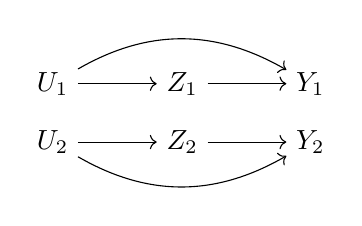
\begin{tikzpicture}
        \node (1) {$U_1$};
		\node[ right= of 1] (2) {$Z_1$};
		\node[ right= of 2] (3) {$Y_1$};
		\node[below =0.2 of 1] (12) {$U_2$};
		\node[ right= of 12] (22) {$Z_2$};
		\node[ right= of 22] (32) {$Y_2$};
		\draw[->] (1) to (2); 
		\draw[->] (12) to (22); 
		\draw[->] (2) to (3); 
		\draw[->] (12) to [out=330,in=210] (32);
		\draw[->] (1) to [out=30,in=150] (3);
		\draw[->] (22) to (32);
\end{tikzpicture}
\end{figure}
and clearly $Z_2$ and $Y_1$ are (unconditonally) independent. Therefore the interference effect on Unit 1 is identified as a contrast of Unit 1 outcomes between pairs that have $Z_2 = 1$ and pairs that have $Z_2 = 0$, since
\[
\iota_1(z) = 0 = \E[Y_1 \mid Z_2 = 1] - \E[Y_1 \mid Z_2 = 0].
\]

\item If $\bm U, \bm Z$ are spatial, $Z_2$ and $Y_1$ are not (unconditionally) independent, and therefore we expect that $\E[Y_1 \mid Z_2 = 1] - \E[Y_1 \mid Z_2 = 0] \neq 0$, which means that it does not identify $\iota_1(z)$.

Here, all backdoor paths from $\bm Z$ to $Y_1$ are blocked by $U_1$. Therefore, interference effects can be identified by controlling for the local value of the exposure and the confounder as
\[
\iota_1(z) = \E \left[ \E(Y_1 \mid Z_1 = z, U_1, Z_2 = 1) - \E(Y_1 \mid Z_1 = z, U_1, Z_2 = 0) \right],
\]
where the outer expectation is with respect to $U_1$.

\end{enumerate}

\end{proof}


\subsection{Graph \ref{fig:general_spatial_conf}: Direct and indirect spatial confounding}

\begin{proposition}[Identifiability of local and interference effects under direct and indirect spatial confounding] For variables with causal relationships depicted in \cref{fig:general_spatial_conf}, the following statements hold:
\begin{enumerate}[leftmargin=*,topsep=3pt,itemsep=0pt]
\item Local and interference effects can be identified by controlling for the local and neighborhood covariate value.
\item When the exposure is inherently spatial, controlling for the neighborhood exposure and the local covariate does not suffice to identify local effects.
\end{enumerate}
\label{supp_prop:general_spatial_conf_identify}
\end{proposition}

\begin{proof}[Proof of \cref{supp_prop:general_spatial_conf_identify}]
We again focus on local and interference effects for Unit 1. Results for the effects on Unit 2 are identical.

\begin{enumerate}[leftmargin=*]
\item
The graph describing this setting is depicted below: 
\begin{figure}[H]
\centering
\begin{tikzpicture}
        \node (1) {$U_1$};
        \node [below left =0.25 and 0.25 of 1] (10) {$U^u$};
        \node [below left =0.25 and 0.25 of 2] (20) {$Z^u$};
		\node[ right= of 1] (2) {$Z_1$};
		\node[ right= of 2] (3) {$Y_1$};
		\node[below = of 1] (12) {$U_2$};
		\node[ right= of 12] (22) {$Z_2$};
		\node[ right= of 22] (32) {$Y_2$};
		\draw[->] (1) to (2); 
		\draw[->] (12) to (22); 
		\draw[->] (2) to (3); 
		\draw[->] (12) to [out=330,in=210] (32);
		\draw[->] (1) to [out=45,in=45,looseness=1.35] (32);
		\draw[->] (12) to [out=315,in=315,looseness=1.35] (3);
		\draw[->] (1) to [out=30,in=150] (3);
		\draw[->] (22) to (32);
		\draw[->] (10) to (1);
		\draw[->] (10) to (12); 
		\draw[->] (20) to (2);
		\draw[->] (20) to (22);
\end{tikzpicture}
\end{figure}

The vector $\bm U$ blocks all backdoor paths from the vector $\bm Z$ to the outcome unit 1, $Y_1$, and therefore it holds that $\bm Z \indep Y_1(z_1, z_2) \mid \bm U$. This implies that
\[
\E[Y_1(z_1, z_2)] = \E \left[ \E(Y_1 \mid Z_1 = z_1, Z_2 = z_2, \bm U) \right],
\]
where the outer expectation is with respect to $\bm U$. Therefore, local and interference effects are identified while controlling for the local and neighborhood covariate.

\item This is a scenario where interference is absent, and we can denote potential outcomes for Unit 1 based only on the treatment of the unit itself, $Y_1(z_1, z_2) = Y_1(z_1)$.
The neighborhood exposure, $Z_2$ is a collider on the backdoor path $Z_1 \leftarrow Z^u \rightarrow Z_2 \leftarrow U_2 \rightarrow Y_1$. Therefore, When $Z_2$ is conditioned on, this backdoor path is open. This implies that $Z_1 \not\indep Y_1(z_1) \mid Z_2, U_1$ and local effects are not identified.

\end{enumerate}


\end{proof}




\subsection{Graph \ref{fig:interference}: Spatial interference}

The definitions of the local and interference effects $\lambda_i(\pi)$ and $\iota_i(\pi)$ that appear in this subsection are given in Supplement \ref{subsec:alternative_definitions_block}.

Propositions \ref{supp_prop:interf_nospat_identif_local} and \ref{supp_prop:interf_nospat_identif_interf} refer to the case of \cref{fig:interference} with $\bm Z$ not spatial. This case corresponds to the graph:
\begin{figure}[H]
\centering
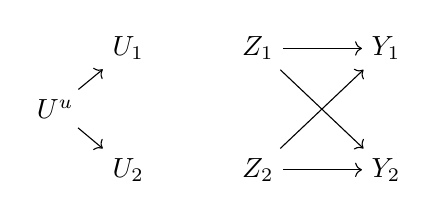
\begin{tikzpicture}
        \node (1) {$U_1$};
        \node [below left =0.25 and 0.25 of 1] (10) {$U^u$};
		\node[ right= of 1] (2) {$Z_1$};
		\node[ right= of 2] (3) {$Y_1$};
		\node[below = of 1] (12) {$U_2$};
		\node[ right= of 12] (22) {$Z_2$};
		\node[ right= of 22] (32) {$Y_2$};
		\draw[->] (2) to (3); 
		\draw[->] (2) to (32);
		\draw[->] (22) to (3);
		\draw[->] (22) to (32);
		\draw[->] (10) to (1);
		\draw[->] (10) to (12); 
\end{tikzpicture}
\end{figure}

\begin{proposition}
For variables with causal relationships depicted in \cref{fig:interference}, if $\bm Z$ is not spatial, then 
$\lambda_1(\pi)$ for $\pi = P(Z_2 = 1)$ is identifiable based on the difference of averages of Unit 1 outcomes for pairs with $Z_1 = 1$ and pairs with $Z_1 = 0$, i.e.,
\[
\lambda_1(\pi) = \E(Y_1 \mid Z_1 = 1) - \E(Y_1 \mid Z_1 = 0)
\]
The case for $\lambda_2(\pi')$, for $\pi' = P(Z_1 = 1)$ is symmetric.
\label{supp_prop:interf_nospat_identif_local}
\end{proposition}

\begin{proof}[Proof of \cref{supp_prop:interf_nospat_identif_local}]
Note that 
\begin{align*}
\lambda_1(\pi)
&= \E [ \pi Y_1(1, 1) - \pi Y_1(0, 1) + (1 - \pi) Y_1(1, 0) - (1 - \pi) Y_1(0, 0)] \\
&= \E [ \pi Y_1(1, 1) + (1 - \pi) Y_1(1, 0)] - \E [ \pi Y_1(0, 1) + (1 - \pi) Y_1(0, 0)],
\end{align*}
so it suffices to identify $\E[ \pi Y_1(z, 1) + (1 - \pi) Y_1(z, 0)]$, for $z = 0, 1$.
The proof is similar to that on Page 566 of \cite{ogburn2014causal}.
\begin{align*}
\E & \left[ \pi Y_1(z, 1) + (1 - \pi) Y_1(z, 0) \right] \\
&= \pi  \E \left[ Y_1(z, 1) \right] + (1 - \pi) \E \left[ Y_1(z, 0) \right] \\
&= \pi  \E \left[ Y_1(z, 1) \mid Z_1 = z, Z_2 = 1 \right] +
(1 - \pi) \E \left[ Y_1(z, 0) \mid Z_1 = z, Z_2 = 0 \right]
\tag{Ignorability} \\
&= \pi  \E \left[ Y_1 \mid Z_1 = z, Z_2 = 1 \right] +
(1 - \pi) \E \left[ Y_1 \mid Z_1 = z, Z_2 = 0 \right]
\tag{Consistency of potential outcomes} \\
&= P(Z_2 = 1)  \E \left[ Y_1 \mid Z_1 = z, Z_2 = 1 \right] +
P(Z_2 = 0) \E \left[ Y_1 \mid Z_1 = z, Z_2 = 0 \right] \\
&= P(Z_2 = 1 \mid Z_1 = z)  \E \left[ Y_1 \mid Z_1 = z, Z_2 = 1 \right] +
P(Z_2 = 0 \mid Z_1 = z) \E \left[ Y_1 \mid Z_1 = z, Z_2 = 0 \right]
\tag{Treatment values are independent} \\
&= \E \left[ Y_1 \mid Z_1 = z \right].
\end{align*}
\end{proof}


\begin{proposition}
For the variables' with causal dependence depicted in \cref{fig:interference}, when the exposure $\bm Z$ is spatial, the difference of averages of Unit 1 outcomes for pairs with $Z_1 = 1$ and pairs with $Z_1 = 0$ does {\it not} identify an interpretable local effect for Unit 1. Interpretable local causal effects for Unit 1 can be identified by adjusting for the neighbor's exposure.
\label{supp_prop:interf_identif_local}
\end{proposition}

\begin{proof}[Proof of \cref{supp_prop:interf_identif_local}]
Following the steps of the proof of \cref{supp_prop:interf_nospat_identif_local} backwards, we have that the average outcome of Unit 1 among pairs with $Z_1 = z$ estimates the quantity
\begin{align*}
\E(Y_1 \mid Z_1 = z)
&= 
P(Z_2 = 1 \mid Z_1 = z)  \E \left[ Y_1(z, 1) \right] +
P(Z_2 = 0 \mid Z_1 = z) \E \left[ Y_1(z, 0) \right]
\end{align*}
where we used consistency of potential outcomes, and that $\bm Z \indep Y_1(z_1, z_2)$ under the causal dependence depicted in the graph \ref{fig:interference}.
This quantity is the average outcome when Unit 1's treatment is set to $z$ and Unit 2's treatment is equal to 1 with probability $P(Z_2 = 1 \mid Z_1 = z)$ and 0 otherwise.

Then, the contrast of average Unit 1 outcomes among pairs with $Z_1 = 1$ and $Z_1 = 0$ estimates the peculiar contrast
\begin{align*}
\E(Y_1 \mid & Z_1 = 1) - \E(Y_1 \mid Z_1 = 0)  = \\ 
&= \left\{ P(Z_2 = 1 \mid Z_1 = 1)  \E \left[ Y_1(1, 1) \right] +
P(Z_2 = 0 \mid Z_1 = 1) \E \left[ Y_1(1, 0) \right] \right\} \\
& \hspace{20pt} - \left\{ P(Z_2 = 1 \mid Z_1 = 0)  \E \left[ Y_1(0, 1) \right] +
P(Z_2 = 0 \mid Z_1 = 0) \E \left[ Y_1(0, 0) \right] \right\},
\end{align*}
where not only Unit 1's treatment changes from 1 to 0, but also the probability of treatment for Unit 2 changes. Therefore, it is unclear whether this estimated quantity has a causal interpretation. At the least, it does not isolate the effect of a change in $Z_1$ and cannot be interpreted as a local causal effect.

Since the ignorability of the (vector) exposure holds unconditionally, $\bm Z \indep Y_1(z_1, z_2)$, we have that Unit 1's local effects defined in \cref{sec:pairs} can be identified when $Z_2$ is adjusted.

\end{proof}

\begin{remark}
When $\bm Z$ is not spatial, $P(Z_2 = 1 \mid Z_1 = z) = P(Z_2 = 1)$, and \cref{supp_prop:interf_identif_local} reverts back to \cref{supp_prop:interf_nospat_identif_local}.
The results in Propositions \ref{supp_prop:interf_nospat_identif_local} and \ref{supp_prop:interf_identif_local} combined establish explicitly how, in this very simple case without any confounding, an identification strategy for local effects can be invalidated by statistical dependence in the exposure variable.
\end{remark}


\begin{proposition}
For variables with causal relationships depicted in \cref{fig:interference}, if $\bm Z$ is not spatial, then $\iota_1(\pi)$ for $\pi = P(Z_1 = 1)$ is identifiable based on the difference of averages of Unit 1 outcomes for pairs with $Z_2 = 1$ and pairs with $Z_2 = 0$. The case for $\iota_2(\pi')$, for $\pi' = P(Z_2 = 1)$ is symmetric.
\label{supp_prop:interf_nospat_identif_interf}
\end{proposition}
\noindent
The proof of \cref{supp_prop:interf_nospat_identif_interf} is identical to the proof of \cref{supp_prop:interf_nospat_identif_local}, hence it is omitted.


\subsection{Graph \ref{fig:predictor_interference}: Interference with spatial predictor of the exposure}

\begin{proposition}
For the variables with causal relationships depicted in \cref{fig:predictor_interference}, the difference of averages of Unit 1 outcomes for pairs with $Z_1 = 1$ and pairs with $Z_1 = 0$ conditionally on $U_1$ and unconditionally identify different quantities, none of which is an interpretable causal effect.
\label{supp_prop:predictor_interf_identif}
\end{proposition}

\begin{proof}[Proof of \cref{supp_prop:predictor_interf_identif}]
We consider again two estimators, one of which is unconditional and the other is conditional on $U_1$. These estimators are of the form
\[
\widehat \tau = \E(Y_1 \mid Z_1 = 1) - \E(Y_1 \mid Z_1 = 0),
\]
and
\[
\widehat \tau^{\mid U} = \E[ \E(Y_1 \mid Z_1 = 1, U_1) - \E(Y_1 \mid Z_1 = 0, U_1)],
\]
respectively, where for the second estimator the outer expectation is with respect to the distribution of $U_1$ across pairs.

For the unconditional estimator, $\widehat \tau$, since $\bm Z \indep Y_1(z_1, z_2)$ under the causal dependencies represented in \ref{fig:predictor_interference}, we can again derive that
\begin{align*}
\widehat \tau &= \E(Y_1 \mid Z_1 = 1) - \E(Y_1 \mid Z_1 = 0)  \\ 
&= \left\{ P(Z_2 = 1 \mid Z_1 = 1)  \E \left[ Y_1(1, 1) \right] +
P(Z_2 = 0 \mid Z_1 = 1) \E \left[ Y_1(1, 0) \right] \right\} \\
& \hspace{20pt} - \left\{ P(Z_2 = 1 \mid Z_1 = 0)  \E \left[ Y_1(0, 1) \right] +
P(Z_2 = 0 \mid Z_1 = 0) \E \left[ Y_1(0, 0) \right] \right\},
\end{align*}
identically to the derivations in the proof of \cref{supp_prop:interf_identif_local}.

Furthermore, since $\bm Z \indep Y_1(z_1, z_2) \mid U_1$ also holds, we can similarly derive that
\begin{align*}
\E[ \E(Y_1 \mid & Z_1 = z, U_1) ] = \\
&= \E\{ P(Z_2 = 1 \mid Z_1 = z, U_1) \ \E[ Y_1(z, 1) \mid U_1] + \\
& \hspace{40pt} + P(Z_2 = 0 \mid Z_1 = z, U_1) \ \E[Y_1(z, 0) \mid U_1] \} \\
&= \E[ P(Z_2 = 1 \mid Z_1 = z, U_1)] \ \E[ Y_1(z, 1) ] + \\
& \hspace{40pt} + \E [P(Z_2 = 0 \mid Z_1 = z, U_1)] \ \E[Y_1(z, 0)],
\end{align*}
where, in the last equation, we have used the fact that $U_1$ does not predict $Y_1$ except through $Z$. Therefore the (conditional) contrast of average outcomes, $\widehat \tau^{\mid U}$ estimates
\begin{align*}
\widehat \tau^{\mid U} 
&= \E[ \E( Y_1 \mid Z_1 = 1, U_1) ] - \E[ \E(Y_1 \mid Z_1 = 0, U_1) ] \\
&= \left\{ \E[ P(Z_2 = 1 \mid Z_1 = 1, U_1)] \ \E[ Y_1(1, 1) ] + \E [P(Z_2 = 0 \mid Z_1 = 1, U_1)] \ \E[Y_1(1, 0)] \right\} - \\
& \hspace{20pt} - 
\left\{
\E[ P(Z_2 = 1 \mid Z_1 = 0, U_1)] \ \E[ Y_1(0, 1) ] + \E [P(Z_2 = 0 \mid Z_1 = 0, U_1)] \ \E[Y_1(0, 0)]
\right\}.
\end{align*}

In general, it holds that
\[
P(Z_2 = 1 \mid Z_1 = z) \neq \E[ P(Z_2 = 1 \mid Z_1 = z, U_1)],
\]
since the outer expectation on the right-hand side is with respect to the (marginal) distribution of $U_1$, rather than the distribution of $U_1$ given $Z_1 = z$. Since these two quantities are different, in general it holds that $\widehat \tau \neq \widehat \tau^{\mid U}$. Therefore, the conditional and unconditional estimators estimate different quantities.

The proof that none of these estimate an interpretable causal effect is identical to the one in the proof of \cref{supp_prop:interf_identif_local}, and it relates to the fact that these contrast consider a distribution for $Z_2$ that changes based on the value of $Z_1$.
\end{proof}


\begin{remark}
From the proof of \cref{supp_prop:predictor_interf_identif}, we can identify some interesting cases where the conditional and unconditional estimators estimate the same quantity, or they return interpretable local causal effects:
%
\begin{itemize}
\item When $\bm Z$ is not spatial, we have that
\[ \E[ P(Z_2 = 1 \mid Z_1 = z, U_1)] = \E[ P(Z_2 = 1 \mid U_1)] = P(Z_2 = 1), \]
and therefore the conditional estimator, $\widehat \tau^{\mid U}$, estimates the interpretable local causal effect $\lambda_1(P(Z_2 = 1))$.
%
\item When $\bm Z$ is not spatial, but the spatial predictor $\bm U$ is present,
\( P(Z_2 = 1 \mid Z_1 = z) \neq P(Z_2 = 1), \)
and the unconditional estimator, $\widehat \tau$, still fails to estimate an interpretable causal effect.
%
\item When $\bm U$ is not spatial, $ \E[ P(Z_2 = 1 \mid Z_1 = z, U_1)] = P(Z_2 = 1 \mid Z_1 = z$, and the two estimators estimate the same quantity.
\end{itemize}
\end{remark}


\subsection{Graph \ref{fig:direct_interference}: Direct spatial confounding and interference}

\begin{proposition}
When the variables' causal relationships are depicted in \cref{fig:direct_interference}, 
\begin{enumerate}[leftmargin=*,topsep=3pt,itemsep=0pt]
\item Controlling for the local confounder and neighborhood exposure suffices to identify local effects.
\item Failing to adjust for the local confounder or the neighborhood exposure returns estimates that cannot be interpreted as causal effects.
\end{enumerate}
\label{supp_prop:direct_interf_ident_local}
\end{proposition}

\begin{proof}[Proof of \cref{supp_prop:direct_interf_ident_local}]
$ $
\begin{enumerate}[leftmargin=*]
\item The local confounder blocks all backdoor paths from $\bm Z$ into $Y_1$. As a result, all potential outcomes of the form $\E[Y_1(z_1, z_2)]$, and hence local (and interference) effects, can be identified.
\item Without conditioning on $U_1$, there is a backdoor path from the vector $\bm Z$ to the outcome $Y_1$, and we have that $\bm Z \not\indep Y_1(z_1, z_2)$. Therefore, local (or interference) effects cannot be identified.

Without conditioning on $Z_2$, this setting is almost identical to the one discussed in \cref{supp_prop:predictor_interf_identif} where $U_1$ is conditioned on or not, and estimated quantities cannot be interpreted as causal effects.
\end{enumerate}
\end{proof}

Next, we focus on identification of interpretable causal effects when the exposure is not spatial. \cref{supp_prop:direct_interf_nospat_identif} shows that, when $\bm Z$ is not spatial, one would need to adjust only for the local confounder in order to acquire interpretable local causal effects, even if interference is present. First, we define these {\it new} type of interpretable effects.

We define conditional average local effects. First, let
\[
\lambda_i(z; u_i) = \E[ Y_i(z_i = 1, z_j = z) - Y_i(z_i = 0, z_j = 0) \mid U_i = u_i]
\]
denote the expected change in unit $i$'s outcome for changes in its own treatment when the neighbor's treatment is set to $z$, among clusters with $U_i = u_i$. This is the equivalent to the local effects defined in \cref{eq:local_effect}, where we now also condition on the unit's covariate values.

We also consider expected conditional average local effects, where we average over a distribution for the neighbor's treatment. Specifically,
let $\pi(u_i) = P(Z_j = 1 \mid U_i = u_i)$. We define
\[
\lambda_i(\pi(u_i) ; u_i) = \pi(u_i) \lambda_i(1; u_i) + (1 - \pi(u_i)) \lambda_i(0; u_i),
\]
representing the average change in unit $i$'s outcome among clusters with $U_i = u_i$ for changes in unit $i$'s own treatment, and when the treatment of its neighbor is distributed according to $\pi(\cdot)$. These effects are the conditional equivalent to effects $\lambda_i(\pi)$ in Supplement \ref{subsec:alternative_definitions_block}.

\begin{proposition}
When the variables' causal relationships can be described in the graph of \cref{fig:direct_interference}, if $\bm Z$ is not spatial, it holds that
\[
\E_{U_1} [\lambda_1(\pi(U_1); U_1)] = \E_{U_1} [ \E \left( Y_1 \mid Z_1 = 1, U_1 \right) - \E \left( Y_1 \mid Z_1 = 0, U_1 \right) ]
\]
The case for $\E_{U_2}[\lambda_2(\pi'(U_2); U_2)]$, for $\pi'(u_2) = P(Z_1 = 1 \mid U_2 = u_2)$ is symmetric.
\label{supp_prop:direct_interf_nospat_identif}
\end{proposition}

\begin{proof}[Proof of \cref{supp_prop:direct_interf_nospat_identif}]
We follow steps that are similar to those in the proof of  \cref{supp_prop:interf_nospat_identif_local}. However, here, we have to account for the fact that we average over a distribution of $\pi(U_1)$.
\begin{align*}
\E_{U_1} & \left[ \E \left( Y_1 \mid Z_1 = 1, U_1 \right) - \E \left( Y_1 \mid Z_1 = 0, U_1 \right) \right] = \\
&= \E_{U_1} \big\{ \big[
\E \left( Y_1 \mid Z_1 = 1, Z_2 = 1, U_1 \right) P(Z_2 = 1 \mid Z_1 = 1, U_1) + \\
& \hspace{100pt}
\E \left( Y_1 \mid Z_1 = 1, Z_2 = 0, U_1 \right) P(Z_2 = 0 \mid Z_1 = 1, U_1)
\big]  -  \\
& \hspace{60pt}
\big[
\E \left( Y_1 \mid Z_1 = 0, Z_2 = 1, U_1 \right) P(Z_2 = 1 \mid Z_1 = 0, U_1) + \\
& \hspace{160pt}
\E \left( Y_1 \mid Z_1 = 0, Z_2 = 0, U_1 \right) P(Z_2 = 0 \mid Z_1 = 0, U_1)
\big] \big\} \\
%
&= \E_{U_1} \big\{ \big[
\E \left( Y_1(1, 1) \mid Z_1 = 1, Z_2 = 1, U_1 \right) P(Z_2 = 1 \mid Z_1 = 1, U_1) + \\
& \hspace{100pt}
\E \left( Y_1(1, 0) \mid Z_1 = 1, Z_2 = 0, U_1 \right) P(Z_2 = 0 \mid Z_1 = 1, U_1)
\big]  -  \\
& \hspace{60pt}
\big[
\E \left( Y_1(0, 1) \mid Z_1 = 0, Z_2 = 1, U_1 \right) P(Z_2 = 1 \mid Z_1 = 0, U_1) + \\
& \hspace{160pt}
\E \left( Y_1(0, 0) \mid Z_1 = 0, Z_2 = 0, U_1 \right) P(Z_2 = 0 \mid Z_1 = 0, U_1)
\big] \big\}
\tag{Consistency of potential outcomes} \\
%
&= \E_{U_1} \big\{ \big[
\E \left( Y_1(1, 1) \mid U_1 \right) P(Z_2 = 1 \mid Z_1 = 1, U_1) + 
\E \left( Y_1(1, 0) \mid U_1 \right) P(Z_2 = 0 \mid Z_1 = 1, U_1)
\big]  -  \\
& \hspace{60pt}
\big[
\E \left( Y_1(0, 1) \mid U_1 \right) P(Z_2 = 1 \mid Z_1 = 0, U_1) +
\E \left( Y_1(0, 0) \mid U_1 \right) P(Z_2 = 0 \mid Z_1 = 0, U_1)
\big] \big\}
\tag{Ignorability $Z_1, Z_2 \indep Y_1(z_1, z_2) \mid U_1$ implied by the graph \ref{fig:direct_interference}} \\
%
&= \E_{U_1} \big\{ \big[
\E \left( Y_1(1, 1) \mid U_1 \right) P(Z_2 = 1 \mid U_1) + 
\E \left( Y_1(1, 0) \mid U_1 \right) P(Z_2 = 0 \mid U_1)
\big]  -  \\
& \hspace{60pt}
\big[
\E \left( Y_1(0, 1) \mid U_1 \right) P(Z_2 = 1 \mid U_1) +
\E \left( Y_1(0, 0) \mid U_1 \right) P(Z_2 = 0 \mid U_1)
\big] \big\}
\tag{$Z_1 \indep Z_2 \mid U_1$ according to the graph \ref{fig:direct_interference}} \\
%
&= \E_{U_1} \big\{ \big[
\E \left( Y_1(1, 1) \mid U_1 \right) \pi(U_1) + 
\E \left( Y_1(1, 0) \mid U_1 \right) (1 - \pi(U_1))
\big]  -  \\
& \hspace{60pt}
\big[
\E \left( Y_1(0, 1) \mid U_1 \right) \pi(U_1) +
\E \left( Y_1(0, 0) \mid U_1 \right) (1 - \pi(U_1))
\big] \big\} \\
%
&= \E_{U_1} \big[ \lambda_1(\pi(U_1); U_1) \big]
\end{align*}
\end{proof}

We can define and identify interference effects similarly, without adjusting for the local exposure value.

\section{Motivating simulation studies}
\label{supp_sec:motivating_sims}


\subsection{Motivating simulation study with paired data}
\label{subsec:illustrate_bias_pairs}

To illustrate the points made in \cref{subsec:pairs_graphs} and show how interference and spatial confounding can manifest as each other and affect estimation of local and interference effects, we perform a small simulation study. We simulate pairs of $\bm U$ from a bivariate Normal distribution with mean 0, and covariance matrix $\Sigma_U = \left( \begin{smallmatrix} 1 & \phi_U \\ \phi_U & 1 \end{smallmatrix} \right)$. We also simulate a bivariate normal error term $\bm \epsilon_Z = (\epsilon_{Z,1}, \epsilon_{Z, 2})$ with marginal variances equal to 1 and correlation parameter $\phi_Z$. The binary exposure is generated from a Bernoulli distribution with a logistic link function and linear predictor $\beta_{UZ} U_i + \epsilon_{Z,i}$. Higher values of $\phi_U, \phi_Z$ correspond to stronger inherent spatial dependence for $\bm U$ and $\bm Z$.
The outcome is generated independently across locations from a normal distribution with mean $\beta_Z Z_i + \beta_{\bar Z} \overline Z_i + \beta_U U_i + \beta_{\bar U} \overline U_i$ and variance 1, where $\overline Z_i$ and $\overline U_i$ represent the value of the exposure and the covariate for the neighbor of location $i$, respectively.
Under this model, $\beta_Z$ and $\beta_{\bar{Z}}$ correspond to the local and interference effects, respectively.
We consider the six different scenarios presented in \cref{fig:graphs} by setting different parameters to zero. 
We simulate 300 data sets of 200 pairs each, and fit ordinary least squares (OLS) using different sets of predictor variables.
The data generating model and hyperparameters for each of these scenarios are listed in Table \ref{tab:pairdata}, along with the bias for the OLS estimators of $\beta_Z$ and $\beta_{\bar{Z}}$.



\begin{table}[p]
\spacingset{1}
\small
\centering
\caption{Motivating Simulation Study with Paired Data. For the graphs of \cref{fig:graphs}, we illustrate the induced biases in estimating local and interference causal effects due to spatial dependencies.
In these simulations, the parameters that drive the data generative mechanism are $\phi_U, \phi_Z, \beta_{UZ}, \beta_Z, \beta_{\bar Z}, \beta_U, \beta_{\bar U}.$ The different scenarios of \cref{fig:graphs} correspond to different set of parameters fixed at 0, shown below. Unless otherwise noted, the parameters are fixed at $\phi_U = 0.7$, $\phi_Z = 0.5, \beta_{UZ} = 1, \beta_Z = 1, \beta_{\bar Z} = 0.8, \beta_U = 1, \beta_{\bar U} = 0.5$. We generate 300 data sets of 200 pairs each. We regress the outcome on a different set of variables (columns), and report the bias of the OLS estimator for the local effect estimator, $\beta_Z$, and the interference effect estimator, $\beta_{\bar Z}$, when $\overline Z$ is included in the conditioning set. Values are rounded to the third decimal point, and those in {\bf bold} are discussed in the main text.
}
\spacingset{1}
    % \rowcolors{5}{}{gray!10}
    \resizebox{0.88\textwidth}{!}{%
    \begin{tabular}{*{10}{c}}
        \hline
        & & & & &  & \\[-12pt]
        & &  \multicolumn{8}{c}{Conditioning set} \\
        \multirow{2}{*}{\shortstack[c]{True \\[5pt] Model}} & \multirow{3}{*}{\shortstack[c]{Alternative \\[5pt] spatial \\[5pt] parameters}} & \multicolumn{8}{c}{\& estimated parameter} \\[2pt]
        \cmidrule{3-10} 
        & & \\[-15pt]
        & &  $(Z) $ & $(Z, U)$  & \multicolumn{2}{c}{  $(Z, \bar{Z})$} & \multicolumn{2}{c}{  $(Z, \bar{Z}, U)$} & \multicolumn{2}{c}{  $(Z, \bar{Z}, U, \bar{U})$}\\
        %\cmidrule(lr){3-3} \cmidrule(lr){4-4} \cmidrule(lr){5-6} \cmidrule(lr) {7-8} \cmidrule(lr) {9-10}
        %& & \\
        %\cmidrule{3-10} 
        \cmidrule(lr){3-3} \cmidrule(lr){4-4} \cmidrule(lr){5-6} \cmidrule(lr) {7-8} \cmidrule(lr) {9-10}
        & & $\beta_Z$ & $\beta_Z$ & $\beta_Z$ & $\beta_{\bar{Z}}$ & $\beta_Z$ & $\beta_{\bar{Z}}$ & $\beta_Z$ & $\beta_{\bar{Z}}$\\
        & & & & & & \\[-8pt]
        \hline \\[-8pt]
%
\multirow{2}{*}{\ref{fig:direct}} & & \multicolumn{8}{c}{$\beta_{\bar Z} = 0$ and $\beta_{\bar U}=0$} \\[2pt]
        \cmidrule{5-8}
        & & 0.726 & -0.003 & 0.660 & {\bf 0.406} & -0.003 & {\bf -0.002} & -0.002 & 0.000  \\
        \midrule \\[-8pt]
%
\multirow{2}{*}{\ref{fig:general_spatial_conf}} & & 
        \multicolumn{8}{c}{$\beta_{\bar Z} = 0$}
        \\[2pt]
        \cmidrule{5-8}
%        & $\phi_z = 0.7$ & 0.909 & -0.007 & 0.816 & 0.601 & -0.036 & 0.297 & -0.006 & 0.004 \\ 
         & %$\phi_z = 0.5$ 
         & 0.983 & 0.002 & 0.863 & 0.737 & -0.013 & {\bf 0.198} & -0.002 & {\bf 0.000}  \\ 
%         & $\phi_z = 0.3 $ & 0.904 & -0.008 & 0.839 & 0.636 & -0.020 & 0.295 & -0.005 & 0.004  \\
         \midrule \\[-8pt]
%
\multirow{4}{*}{\ref{fig:interference}} & & 
\multicolumn{8}{c}{$\beta_{UZ} = 0$ and $\beta_U = \beta_{\bar U} = 0$}
        \\[2pt]
        \cmidrule{5-8}
        & $\phi_z = 0.7$ & {\bf 0.152} & 0.087 & 0.001 & -0.002 & -0.001 & -0.003 & 0.000 & -0.002  \\
         & $\phi_z = 0.5$ & {\bf 0.129} & 0.060 & -0.001 & -0.001 & -0.003 & -0.002 & -0.002 & 0.000 \\
        & $\phi_z = 0.3$ & {\bf 0.105} & 0.032 & -0.002 & 0.001 & -0.003 & 0.000 & -0.003 & 0.001 \\
        \midrule \\[-8pt]
%
\multirow{4}{*}{\ref{fig:predictor_interference}} & 
& \multicolumn{8}{c}{$\beta_U = 0$ and $\beta_{\bar U} = 0$} \\[2pt]
\cmidrule{5-8}
        & $\beta_{UZ} = 1.5$ & {\bf 0.173} & {\bf 0.052} & 0.000 & 0.001 & -0.002 & 0.000 & -0.002 & 0.003 \\
        & $\beta_{UZ} = 1\phantom{.a}$ &  0.129 & 0.060 & -0.001 & -0.001 & -0.003 & -0.002 & -0.002 & 0.000  \\
        & $\beta_{UZ} = 0.5$ & 0.083 & 0.061 & -0.004 & -0.003 & -0.006 & -0.004 & -0.005 & -0.003 \\
\midrule \\[-8pt]
%
\multirow{3}{*}{\ref{fig:direct_interference}} & & 
\multicolumn{8}{c}{$\beta_{\bar U} = 0$} \\[2pt]
        \cmidrule{5-8}
& $\phi_Z = 0.5$ & 0.856 & {\bf 0.060} & 0.660 & 0.406 & -0.003 & -0.002 & -0.002 & 0.000 \\ 
& $\phi_Z = 0\phantom{.5}$ & 0.800 & {\bf -0.001} & 0.684 & 0.445 & 0.000 & -0.003 & 0.000 & -0.001 \\
\midrule \\[-8pt]
%
\ref{fig:general_interference}
         & & 1.113 & 0.064 & 0.863 & 0.737 & -0.013 & 0.198 & -0.002 & 0.000 \\
        & & & & & &  \\[-8pt]
          \hline
        \end{tabular}
     }%
\label{tab:pairdata}
\end{table}

In the presence of only direct spatial confounding (Scenario \ref{fig:direct}), we see that failing to adjust for the local spatial confounder returns biased interference effect estimates ($\beta_{\bar Z}$ in the model with $Z, \overline Z$ in \cref{tab:pairdata}). Therefore, in the presence of inherently spatial data, adjusting for spatial confounders is crucial for learning interference effects, even if spatial confounding is direct only. When spatial confounding is both direct and indirect (Scenario \ref{fig:general_spatial_conf}), adjusting only for the local spatial confounder and exposure values can still return misleading interference effects ($\beta_{\bar Z}$ in the model with $Z, \overline Z, U$), and it is necessary to also account for the neighbor's covariate value. In the presence of interference (Scenario \ref{fig:interference}) and when the exposure is inherently spatial, the local effect estimator is biased when the neighbor's exposure value is not conditioned on, and the bias is larger for stronger spatial dependence. Instead, local and interference effects can be unbiasedly estimated when they are considered simultaneously ($\beta_Z, \beta_{\bar Z}$ in the model with $Z, \overline Z$).
In Scenario \ref{fig:predictor_interference}, the local effect of the exposure for unit $i$ is biased regardless of whether $U_i$ is adjusted for or not. At the same time, the estimates when $U_i$ is included in the model or not are substantially different, which could be interpreted as $U_i$ confounding the local effect. Therefore, in this scenario, the inherent spatial structure in the confounders and exposure could lead to  interference being mistakenly interpreted as spatial confounding.
In Scenario \ref{fig:direct_interference}, we see that when the exposure is not inherently spatial ($\phi_Z = 0$), we can learn local effects without adjusting for the neighbor's exposure. However, this estimator is biased when the exposure has an inherent spatial structure, illustrating practically that spatial dependencies can hinder some analyses invalid if not properly taken into account.
Of course, when all the possible dependencies are present in Scenario \ref{fig:general_interference}, one would need to condition on local and neighborhood covariates to properly estimate local and interference effects. The estimator that account for all of local and neighborhood exposure and confounding values returns unbiased effect estimates across all scenarios.



\subsection{Motivating simulation study in a setting with one spatial network of observations}
\label{supp_sec:motivating_one_network}

We consider a graph with $n$ nodes. We assume that this graph is a line graph, in that the first and last nodes are connected only to the second and second to last, respectively, and node $i$ is connected to nodes $i - 1$ and $i + 1$ for $i = 2, 3, \dots, n-1$. This implies the following adjacency and degree matrices:
\[
A = \begin{pmatrix}
0 & 1 & 0 & 0 & \dots & 0 & 0 & 0 \\
1 & 0 & 1 & 0 & \dots & 0 & 0 & 0 \\
0 & 1 & 0 & 1 & \dots & 0 & 0 & 0 \\
& & \vdots & & \dots & & \vdots &  \\
0 & 0 & 0 & 0 & \dots & 1 & 0 & 1 \\
0 & 0 & 0 & 0 & \dots & 0 & 1 & 0 
\end{pmatrix} \quad \text{and} \quad
D = \begin{pmatrix}
1 & 0 & 0 & \dots & 0 & 0 \\
0 & 2 & 0 & \dots & 0 & 0 \\
0 & 0 & 2 & \dots & 0 & 0 \\
& & \vdots & \dots & \vdots & \\
0 & 0 & 0 & \dots & 2 & 0 \\
0 & 0 & 0 & \dots & 0 & 1
\end{pmatrix}.
\]
We generate $\bm U = (U_1, U_2, \dots, U_n)$ and $\bm Z = (Z_1, Z_2, \dots, Z_n)$ simultaneously from a multivariate normal distribution as follows
\[
\begin{pmatrix} \bm U \\ \bm Z \end{pmatrix} \sim N_{2n} \left( \bm 0_{2n},
\begin{pmatrix} G & Q \\ Q & H \end{pmatrix}^{-1}
\right),
\]
where $\bm 0_{2n}$ is a vector of length $2n$ of all $0$s. We specify $G$ and $H$ according to a conditional autoregressive distribution as $G = \tau_U^2 (D - \phi_U A)$ and $H = \tau_Z ^2 (D - \phi_Z A)$. Then, $Q$ is specified to be diagonal with elements $Q_{ii} = - \rho \sqrt{G_{ii} H_{ii}}.$ Note that different values of $\phi$ for the same value of $\tau$ lead to different marginal variances for the entries of $\bm U$ and $\bm Z$.

We exclude measured covariates for simplicity. Once $\bm U$ and $\bm Z$ are generated, the outcome is generated according to the model \cref{eq:linear_sem}, where $\epsilon \sim N(0, 1)$ independent.
Unless otherwise specified, the hyperparameters for these simulations are set to the values reported in \cref{tab:motivating_network}.



\begin{table}[p]
\centering
\spacingset{1}
\caption{
Motivating Simulation Study with One Interconnected Network. Unless otherwise noted, the parameters are fixed at $\phi_U = 0.6$, $\phi_Z = 0.4$, $\tau_U = \tau_Z = 1$, $\rho = 0.35$, $\beta_Z = 1, \beta_{\bar Z} = 0.8, \beta_U = 1, \beta_{\bar U} = 0.5$. We generate 200 data sets with $n = 100$. We regress the outcome on a different set of variables (columns), and report the bias of the OLS estimator for the local effect estimator, $\beta_Z$, and the interference effect estimator, $\beta_{\bar Z}$, when $\overline Z$ is included in the conditioning set. Values are rounded to the third decimal point. We bold the entries corresponding to the same cells as in \cref{tab:pairdata}. The qualitative conclusions remain unchanged.}
    % \rowcolors{5}{}{gray!10}
    \resizebox{0.82\textwidth}{!}{%
    \begin{tabular}{*{10}{c}}
        \hline
        & & & & &  & \\[-5pt]
        & &  \multicolumn{8}{c}{Conditioning set} \\
        \multirow{2}{*}{\shortstack[c]{True \\[5pt] Model}} & \multirow{3}{*}{\shortstack[c]{Alternative \\[5pt] spatial \\[5pt] parameters}} & \multicolumn{8}{c}{\& estimated parameter} \\[5pt]
        \cmidrule{3-10} 
        & & \\[-5pt]
        & &  $(Z) $ & $(Z, U)$  & \multicolumn{2}{c}{  $(Z, \bar{Z})$} & \multicolumn{2}{c}{  $(Z, \bar{Z}, U)$} & \multicolumn{2}{c}{  $(Z, \bar{Z}, U, \bar{U})$}\\
        \cmidrule(lr){3-3} \cmidrule(lr){4-4} \cmidrule(lr){5-6} \cmidrule(lr) {7-8} \cmidrule(lr) {9-10}
        & & $\beta_Z$ & $\beta_Z$ & $\beta_Z$ & $\beta_{\bar{Z}}$ & $\beta_Z$ & $\beta_{\bar{Z}}$ & $\beta_Z$ & $\beta_{\bar{Z}}$\\
        & & & & & & \\[-5pt]
        \hline \\[-5pt]
%
\multirow{2}{*}{\ref{fig:direct}} & & \multicolumn{8}{c}{$\beta_{\bar Z} = 0$ and $\beta_{\bar U}=0$} \\[5pt]
        \cmidrule{5-8}
        & & 0.550 & -0.005 & 0.428 & {\bf 0.370} & -0.007 & {\bf 0.006} & -0.007 & -0.004  \\
        \midrule \\[-5pt]
%
\multirow{2}{*}{\ref{fig:general_spatial_conf}} & & 
        \multicolumn{8}{c}{$\beta_{\bar Z} = 0$}
        \\[5pt]
        \cmidrule{5-8}
%        & $\phi_z = 0.7$ & 0.909 & -0.007 & 0.816 & 0.601 & -0.036 & 0.297 & -0.006 & 0.004 \\ 
         & %$\phi_z = 0.5$ 
         & 0.683 & 0.045 & 0.489 & 0.595 & -0.008 & {\bf 0.237} & -0.013 & {\bf 0.030} \\ 
%         & $\phi_z = 0.3 $ & 0.904 & -0.008 & 0.839 & 0.636 & -0.020 & 0.295 & -0.005 & 0.004  \\
         \midrule \\[-5pt]
%
%
\multirow{4}{*}{\ref{fig:interference}} & & 
\multicolumn{8}{c}{$\rho = 0$ and $\beta_U = \beta_{\bar U} = 0$}
        \\[5pt]
        \cmidrule{5-8}
        & $\phi_z = 0.6$ & {\bf 0.437} & 0.334 & -0.012 & 0.000 & -0.007 & 0.002 & -0.007 & 0.011 \\
         & $\phi_z = 0.4$ & {\bf 0.261} & 0.193 & -0.002 & -0.008 & 0.003 & -0.004 & 0.002 & -0.007 \\
        & $\phi_z = 0.2$ & {\bf 0.151} & 0.088 & 0.006 & -0.002 & 0.002 & -0.005 & 0.003 & 0.000 \\
        \midrule \\[-5pt]
%
\multirow{4}{*}{\ref{fig:predictor_interference}} & 
& \multicolumn{8}{c}{$\beta_U = 0$ and $\beta_{\bar U} = 0$} \\[5pt]
\cmidrule{5-8}
        & $\rho = 0.15$ & 0.183 & 0.170 & 0.003 & 0.003 & 0.004 & 0.005 & 0.004 & 0.002 \\
        & $\rho = 0.35$ & 0.275 & 0.186 & 0.011 & -0.012 & 0.004 & -0.018 & 0.004 & -0.018  \\
        & $\rho = 0.45$ & {\bf 0.431} & {\bf 0.246} & 0.014 & -0.009 & 0.013 & -0.011 & 0.012 & -0.011 \\
        \midrule \\[-5pt]
%
\multirow{3}{*}{\ref{fig:direct_interference}} & & 
\multicolumn{8}{c}{$\beta_{\bar U} = 0$} \\[5pt]
        \cmidrule{5-8}
& $\phi_Z = 0.4$ & 0.838 & {\bf 0.195} & 0.456 & 0.345 & 0.001 & 0.021 & 0.001 & 0.019 \\ 
& $\phi_Z = 0\phantom{.5}$ & 0.501 & {\bf -0.010} & 0.444 & 0.283 & 0.001 & -0.017 & 0.001 & -0.019 \\
\midrule \\[-5pt]
%
\ref{fig:general_interference}
         & & 0.973 & 0.222 & 0.507 & 0.611 & -0.008 & 0.209 & -0.014 & -0.002 \\
        & & & & & &  \\
          \hline
          
        \end{tabular}
     }%
\label{tab:motivating_network}
\end{table}


\section{Identifiability of model parameters}
\label{supp_sec:identifiability_ours}

\begin{proof}[Proof of \cref{theorem:identifiability}]

Consider a spatial network of observations that are organized on a ring graph, with symmetric adjacency matrix $A_{ij} = 1$ if $|i-j| = 1$, $(i = 1, j=n)$ and $(i =n, j=1)$, and 0 otherwise. Intuitively, under this structure, each unit has two neighbors, the ones with adjacent indices, and units 1 and $n$ are connected. 

Without loss of generality, we consider the case without measured covariates and where the exposure has mean 0.
% We have that
% %
% \begin{align*}
% \E[Y(z, \overline z)]
% &= \E\left\{ \E \left[Y(z, \overline z) \mid U,  \overline U \right] \right\} \\
% &= \E\left[ \E \left( Y \mid U, \overline U, Z = z, \overline Z = \overline z \right) \right] \tag{From \cref{ass:network_ignorability} and consistency of potential outcomes} \\
% &= \E\left( \beta_0 + \beta_Z z + \beta_{\bar Z} \overline z + U + \beta_{\bar U} \overline U \right) \\
% &= \beta_0 + \beta_Z z + \beta_{\bar Z} \overline z + \E\left( U + \beta_{\bar U} \overline U \right),
% \end{align*}
% therefore causal effects of the form 
% $\E[Y(z, \overline z)] - \E[Y(z', \overline z')]$ can be identified based on the regression coefficients.
We show that all coefficients, parameters in the precision matrix, and residual variance are identifiable, hence the causal effects of interest are also identifiable.


\paragraph{A few useful derivations}

\begin{itemize}[leftmargin=*]
\item We can write $\overline {\bm U} = D^{-1} A \bm U$ and $\overline {\bm Z} = D^{-1}A \bm Z$, where $D$ is the degree and $A$ is the adjacency matrix. 

\item We have that
\[
\begin{pmatrix}
G & Q \\ Q^\top & H
\end{pmatrix}^{-1} = 
\begin{pmatrix}
G^{-1} + G^{-1} Q (H - Q^\top G^{-1} Q)^{-1} Q^\top G^{-1} &
- G^{-1} Q (H - Q^\top G^{-1} Q)^{-1} \\
- (H - Q^\top G^{-1} Q)^{-1} Q^\top G^{-1} & (H - Q^\top G^{-1} Q)^{-1} 
\end{pmatrix},
\]
and using the known formulas for the multivariate normal distribution, we have that
\[
\bm U \mid \bm Z \sim N(-G^{-1}Q\bm Z, G^{-1}).
\]
\item The diagonal elements of the diagonal matrix $Q$ are $Q_{ii} = - \rho \sqrt{g_{ii} h_{ii}}$. Under the CAR form of $G = \tau_U^2 (D - \phi_U A)$ and $H = \tau_Z^2 (D - \phi_Z A)$, we have that $Q_{ii} = -2 \rho \tau_U \tau_Z$. These imply that
\[
G^{-1}Q = -2 \rho \tau_U \tau_Z G^{-1}.
\]

\item 
Putting these together, we have that
\begin{align*}
\E( \bm Y \mid \bm Z) 
&= \beta_Z \bm Z + \beta_{\bar Z} \overline {\bm Z} + \E[\bm U \mid \bm Z] + \beta_{\bar U} \E[\overline {\bm U} \mid \bm Z] \\
&= \beta_Z \bm Z + \beta_{\bar Z} D^{-1} A \bm Z
- G^{-1} Q \bm Z  + \beta_{\bar U} D^{-1} A (- G^{-1} Q \bm Z) \\
&= \beta_Z \bm Z + \beta_{\bar Z} (D^{-1} A \bm Z) + 2\rho\tau_U \tau_Z ( G^{-1} \bm Z)  + 2 \rho \tau_U \tau_Z \beta_{\bar U} (D^{-1} A G^{-1} \bm Z).
\numberthis
\label{supp_eq:EYmidZ}
\end{align*}
%
and that
%
\begin{align*}
\Var(\bm Y \mid \bm Z) &= \Var [ (I_n + \beta_{\bar U} D^{-1}A ) U \mid Z] + \sigma^2_Y I_n \\
&= (I_n + \beta_{\bar U} D^{-1}A ) \Var(\bm U \mid \bm Z) (I_n + \beta_{\bar U} D^{-1}A )^\top + \sigma^2_Y I_n \\
&= (I_n + \beta_{\bar U} D^{-1}A ) G^{-1} (I_n + \beta_{\bar U} D^{-1}A )^\top + \sigma^2_Y I_n,
\numberthis
\label{supp_eq:VarYmidZ}
\end{align*}
where
\[
I_n + \beta_{\bar U} D^{-1}A = \begin{pmatrix}
    1 & \frac{\beta_{\bar U}}2 &  &  & \dots &  & & \frac{\beta_{\bar U}}2 \\
    \frac{\beta_{\bar U}}2 & 1 & \frac{\beta_{\bar U}}2 &  & \dots &  &  \\
     & \frac{\beta_{\bar U}}2 & 1 & \frac{\beta_{\bar U}}2 & \dots \\
    & & & &  \vdots \\
     & & & &  \dots & \frac{\beta_{\bar U}}2 & 1 &     \frac{\beta_{\bar U}}2 \\
    \frac{\beta_{\bar U}}2 & & & &  \dots & & \frac{\beta_{\bar U}}2 & 1
\end{pmatrix}
\]

\end{itemize}

\paragraph{}
Theorem 1 of \cite{schnell2020mitigating} shows that we can identify whether $\rho\phi_U = 0$ or not based on $\bm Z$. If $\rho\phi_U \neq 0$, they show that $(\tau_Z, \phi_Z, \phi_U, |\rho|)$ are identifiable. Their theorem applies here directly since their results are based on the same specification of the joint distribution $(\bm Z, \bm U)$ on the ring graph.

Our proof deviates from theirs on the specification of the outcome structure and, as a result, the identifiability results for the remaining parameters. These differences stem from allowing for potential interference effects and for including additional parameters on the unmeasured spatial confounder due to non-local confounding, which leads to the inclusion of additional terms and additional unknown parameters in the distribution of $\bm Y$ given $\bm Z$ in equations \cref{supp_eq:EYmidZ} and \cref{supp_eq:VarYmidZ}.

In linear models, expectations and variances are separately identifiable. So we can identify $\Var(\bm Y \mid \bm Z)$ and $\E(\bm Y \mid \bm Z)$.

\paragraph{Identifiability of parameters from $\Var(\bm Y \mid \bm Z)$}

We acquire the form of the entries in $G^{-1}$ as $n \rightarrow \infty$ based on Theorem 4 in the Supplementary Materials of \cite{schnell2020mitigating}. Let entry $(i, j)$ of matrix $G^{-1}$ be denoted by $g_{ij}$. Then, we have that
\begin{align}
\lim_{n \rightarrow \infty} g_{ij}
= 
\frac{\tau_U^2}{2 \sqrt{1 - \phi_U^2}} \left( \frac{\phi_U}{1 + \sqrt{1 - \phi_U^2}} \right)^{|i-j|}
\label{supp_eq:Ginv}
\end{align}
After some mundane matrix multiplications, we have that the entries of the variance in 
\cref{supp_eq:VarYmidZ} can be written as
\begin{align*}
[\Var(\bm Y \mid \bm Z)]_{ij} &= g_{ij} + \frac{\beta_{\bar U}}2 (g_{(i-1)j} + g_{(i+1)j} + g_{i(j-1)} + g_{i(j+1)}) + \\
& \hspace{20pt} + \frac{\beta_{\bar U}^2}4
(g_{(i-1)(j-1)} + g_{(i-1)(j+1)} + g_{(i+1)(j-1)} + g_{(i+1)(j+1)})
+ \sigma^2_Y I(i = j).
\end{align*}
%
Therefore, we can write the limit of the $(i,j)$ entry for the outcome conditional variance $\lim_{n \rightarrow \infty} \Var(\bm Y \mid \bm Z)_{ij}$ as a function of $k = |i-j|$:

\begin{itemize}[leftmargin=*]
\item
For $k = 0$, and $i = j$:
\end{itemize}
%
%
\begin{align*}
\lim_{n \rightarrow \infty} \Var(\bm Y \mid \bm Z)_{ij} 
&= \frac{\tau_U^2}{2 \sqrt{1 - \phi_U^2}} + 4 \frac{\beta_{\bar U}}2 \frac{\tau_U^2}{2 \sqrt{1 - \phi_U^2}} \frac{\phi_U}{1 + \sqrt{1 - \phi_U^2}}
\\
& \quad
+ 4 \frac{\beta_{\bar U}^2}4 \frac{\tau_U^2}{2 \sqrt{1 - \phi_U^2}} \left( \frac{\phi_U}{1 + \sqrt{1 - \phi_U^2}} \right)^2 + \sigma^2_Y \\
%
&= \frac{\tau_U^2}{2 \sqrt{1 - \phi_U^2}} \left[ 1 + 2 \beta_{\bar U}  \frac{\phi_U}{1 + \sqrt{1 - \phi_U^2}} + \beta_{\bar U}^2 \left(\frac{\phi_U}{1 + \sqrt{1 - \phi_U^2}} \right)^2 \right] + \sigma^2_Y \\
%
&= \frac{\tau_U^2}{2 \sqrt{1 - \phi_U^2}} \left[ 1 + \beta_{\bar U}  \frac{\phi_U}{1 + \sqrt{1 - \phi_U^2}} \right]^2 + \sigma^2_Y
\end{align*}

\begin{itemize}[leftmargin=*]
\item For $k = 1$:
\end{itemize}
\begin{align*}
\lim_{n \rightarrow \infty} \Var(\bm Y \mid \bm Z)_{ij} &=
\frac{\tau_U^2}{2 \sqrt{1 - \phi_U^2}} \frac{\phi_U}{1 + \sqrt{1 - \phi_U^2}} + \\
& \quad 
+\frac{\beta_{\bar U}}2 \left[ 2 \frac{\tau_U^2}{2 \sqrt{1 - \phi_U^2}} +
2 \frac{\tau_U^2}{2 \sqrt{1 - \phi_U^2}} \left( \frac{\phi_U}{1 + \sqrt{1 - \phi_U^2}} \right)^2\right] + \\
& \quad +\frac{\beta_{\bar U}^2}4
\left[ 3 \frac{\tau_U^2}{2 \sqrt{1 - \phi_U^2}} \frac{\phi_U}{1 + \sqrt{1 - \phi_U^2}}  + \frac{\tau_U^2}{2 \sqrt{1 - \phi_U^2}} \left( \frac{\phi_U}{1 + \sqrt{1 - \phi_U^2}} \right)^3 \right] \\
%
%
&=
\frac{\tau_U^2}{2 \sqrt{1 - \phi_U^2}} \left\{ \frac{\phi_U}{1 + \sqrt{1 - \phi_U^2}}+ \beta_{\bar U} \left[ 1 + \left( \frac{\phi_U}{1 + \sqrt{1 - \phi_U^2}} \right)^2 \right] \right. + \\
& \left. \hspace{100pt} +\frac{\beta_{\bar U}^2}4
\left[ 3 \frac{\phi_U}{1 + \sqrt{1 - \phi_U^2}}  + \left( \frac{\phi_U}{1 + \sqrt{1 - \phi_U^2}} \right)^3 \right] \right\}
\end{align*}

\begin{itemize}[leftmargin=*]
\item For $k \geq 2$:
\end{itemize}
\begin{align*}
%%%%%% for k >= 2
& \lim_{n \rightarrow \infty} \Var(\bm Y \mid \bm Z)_{ij} = \\
&=
\frac{\tau_U^2}{2 \sqrt{1 - \phi_U^2}} \left( \frac{\phi_U}{1 + \sqrt{1 - \phi_U^2}} \right)^k + \\
&\quad 
+\frac{\beta_{\bar U}}2 \left[ 2 \frac{\tau_U^2}{2 \sqrt{1 - \phi_U^2}}\left( \frac{\phi_U}{1 + \sqrt{1 - \phi_U^2}} \right)^{k -1} +
2 \frac{\tau_U^2}{2 \sqrt{1 - \phi_U^2}} \left( \frac{\phi_U}{1 + \sqrt{1 - \phi_U^2}} \right)^{k+1} \right] + & \\[10pt]
& \quad +\frac{\beta_{\bar U}^2}4
\left[ 2 \frac{\tau_U^2}{2 \sqrt{1 - \phi_U^2}} \left(\frac{\phi_U}{1 + \sqrt{1 - \phi_U^2}}\right)^k  + \frac{\tau_U^2}{2 \sqrt{1 - \phi_U^2}} \left( \frac{\phi_U}{1 + \sqrt{1 - \phi_U^2}} \right)^{k-2} +
\right. \\[10pt]
& \hspace{200pt} \left.
+ \frac{\tau_U^2}{2 \sqrt{1 - \phi_U^2}} \left( \frac{\phi_U}{1 + \sqrt{1 - \phi_U^2}} \right)^{k + 2} \right] \\
%
%
&=
\frac{\tau_U^2}{2 \sqrt{1 - \phi_U^2}} \left\{ \left( \frac{\phi_U}{1 + \sqrt{1 - \phi_U^2}} \right)^k + \right. \\
&
\hspace{60pt}
+\beta_{\bar U} \left[ \left( \frac{\phi_U}{1 + \sqrt{1 - \phi_U^2}} \right)^{k -1} +
\left( \frac{\phi_U}{1 + \sqrt{1 - \phi_U^2}} \right)^{k+1} \right] + & \\
& 
\hspace{60pt}
\left. +\frac{\beta_{\bar U}^2}4
\left[ 2 \left(\frac{\phi_U}{1 + \sqrt{1 - \phi_U^2}}\right)^k  + \left( \frac{\phi_U}{1 + \sqrt{1 - \phi_U^2}} \right)^{k-2} +
\left( \frac{\phi_U}{1 + \sqrt{1 - \phi_U^2}} \right)^{k + 2} \right] \right\} \\
%
%
&=
\frac{\tau_U^2}{2 \sqrt{1 - \phi_U^2}} \left\{ \left( \frac{\phi_U}{1 + \sqrt{1 - \phi_U^2}} \right)^k + \right. \\
&
\hspace{90pt}
+\beta_{\bar U} \left( \frac{\phi_U}{1 + \sqrt{1 - \phi_U^2}} \right)^{k -1} \left[ 1 +
\left( \frac{\phi_U}{1 + \sqrt{1 - \phi_U^2}} \right)^2 \right] + & \\
& 
\hspace{90pt}
\left. +\frac{\beta_{\bar U}^2}4
\left(\frac{\phi_U}{1 + \sqrt{1 - \phi_U^2}}\right)^{k-2}
\left[ 1 +
\left( \frac{\phi_U}{1 + \sqrt{1 - \phi_U^2}} \right)^2 \right]^2 \right\} \\
%
%
&=
\frac{\tau_U^2}{2 \sqrt{1 - \phi_U^2}}
\left(\frac{\phi_U}{1 + \sqrt{1 - \phi_U^2}}\right)^{k-2}
\left\{ \left( \frac{\phi_U}{1 + \sqrt{1 - \phi_U^2}} \right)^2 + \right. \\
&
\hspace{200pt}
+\beta_{\bar U} \frac{\phi_U}{1 + \sqrt{1 - \phi_U^2}} \left[ 1 +
\left( \frac{\phi_U}{1 + \sqrt{1 - \phi_U^2}} \right)^2 \right] + & \\
& 
\hspace{200pt}
\left. +\frac{\beta_{\bar U}^2}4
\left[ 1 +
\left( \frac{\phi_U}{1 + \sqrt{1 - \phi_U^2}} \right)^2 \right]^2 \right\} \\
%
%
&=
\frac{\tau_U^2}{2 \sqrt{1 - \phi_U^2}}
\left(\frac{\phi_U}{1 + \sqrt{1 - \phi_U^2}}\right)^{k-2}
\left\{ \frac{\phi_U}{1 + \sqrt{1 - \phi_U^2}} 
+
\frac{\beta_{\bar U}}2
\left[ 1 +
\left( \frac{\phi_U}{1 + \sqrt{1 - \phi_U^2}} \right)^2 \right] \right\}^2
\end{align*}

The parameter $\phi_U$ has been identified based on $\bm Z$. Identifiability of $\phi_U$ can also be achieved by comparing the variances of pairs at distance $k$ and $k'$ (when $k, k' \geq 2$), since for a pair $(i,j)$ with distance $k$ (e.g., $|i-j| = k$), and a pair $(i',j')$ with distance $k'$ (e.g., $|i'-j'| = k'$), we have that
\[
\lim_{n \rightarrow \infty} \frac{\Var(\bm Y \mid \bm Z)_{i'j'}}{\Var(\bm Y \mid \bm Z)_{ij}} = \left( \frac{\phi_U}{1 + \sqrt{1 - \phi_U^2}} \right)^{k'-k}.
\]
Therefore, the spatial parameter $\phi_U$ can be identified by studying how spatial correlation in the outcome attenuates with distance.

Once $\phi_U$ is identified, we can identify $\beta_{\bar U}$ by comparing the variances of pairs at distance 1 (pair $(i,j)$ with $|i-j| = k$) with that of pairs at distance 2 (pair $(i',j')$ with $|i'-j'| = 2$), for which
\[
\lim_{n \rightarrow \infty} \frac{\Var(\bm Y \mid \bm Z)_{i'j'}}{\Var(\bm Y \mid \bm Z)_{ij}} =
\frac
{
\left\{ \frac{\phi_U}{1 + \sqrt{1 - \phi_U^2}} 
+
\frac{\beta_{\bar U}}2
\left[ 1 +
\left( \frac{\phi_U}{1 + \sqrt{1 - \phi_U^2}} \right)^2 \right] \right\}^2}
{ \frac{\phi_U}{1 + \sqrt{1 - \phi_U^2}}+ \beta_{\bar U} \left[ 1 + \left( \frac{\phi_U}{1 + \sqrt{1 - \phi_U^2}} \right)^2 \right]  +\frac{\beta_{\bar U}^2}4
\left[ 3 \frac{\phi_U}{1 + \sqrt{1 - \phi_U^2}}  + \left( \frac{\phi_U}{1 + \sqrt{1 - \phi_U^2}} \right)^3 \right] }
\]
is a bijective function of the parameter $\beta_{\bar U}$. Once $\beta_{\bar U}$ is identified, $\tau_U$ can be trivially identified based on the variance of pairs at distance 1 $(|i-j|=1)$. Subsequently, the residual variance $\sigma^2_Y$ can be identified based on the diagonal elements of the covariance matrix $(i = j)$.


\paragraph{Identifiability of parameters from $\E(\bm Y \mid \bm Z)$}

As long as the linear predictors in $\E(\bm Y \mid \bm Z)$ are not perfectly collinear, their corresponding coefficients are identifiable. These linear predictors are $\bm Z, \overline {\bm Z} = D^{-1}A \bm Z$, $G^{-1} \bm Z$, and $D^{-1}A (G^{-1} \bm Z)$, where all parameters in $G$ have been identified.
We assume that the vector $\bm Z$ is not constant, and there is some variation in the exposure across units. Then, the local and neighborhood exposures are not perfectly correlated, and the first two predictors are not collinear. Note that a unit's entry in $\overline {\bm Z}$ is the average of the values in $\bm Z$ for its two neighbors. Based on the form of $G^{-1}$, we see that a unit's entry in $G^{-1}\bm Z$ corresponds to a weighted average of entries in $\bm Z$ of all other units, with weights specified according to \cref{supp_eq:Ginv}, which means that $G^{-1}\bm Z$ is not collinear with the previous ones. Lastly, the same argument holds for $D^{-1}A G^{-1}\bm Z$, as long as $G^{-1} \bm Z$ is not constant across units.

From \cref{supp_eq:EYmidZ}, we have that the coefficients $(\beta_Z, \beta_{\bar Z}, \rho\tau_U\tau_Z, \rho\tau_U\tau_Z\beta_{\bar U})$ are identifiable. Since $\tau_U$ and $\tau_Z$ have already been identified, we now have that the parameter $\rho$ is identifiable as well.

\end{proof}




\section{Illustration of prior distributions}
\label{supp_sec:priors}

As discussed in \cref{subsec:priors}, the prior specifications on the spatial parameters $\tau_U, \tau_Z$ have implications on the implied prior on the the confounding strength due to $U$ and the variance of the  exposure $Z$, respectively. Here, we provide a simulation-based illustration for the implied prior properties discussed in the manuscript.

Before we delve into this illustration, we discuss briefly the matrices $G, H$ in the joint precision matrix of \cref{ass:UZ_normal}, which in the absence of measured covariates states that
\begin{equation}
\begin{pmatrix} \bm U \\ \bm Z \end{pmatrix} \Big| \sim N_{2n} \left(
\bm 0_{2n} ,
\begin{pmatrix} G & Q \\ Q & H \end{pmatrix}^{-1}
\right).
\label{supp_eq:UZ_normal_no_covs}
\end{equation}
Since the joint distribution is parameterized through its precision matrix, $G^{-1}$ and $H^{-1}$ are the marginal covariance matrices of $\bm U$ and $\bm Z$, respectively, {\it only} when $\rho = 0$, and
%generating $\bm U$ from $N_n(\bm 0_n, G^{-1})$ is only in agreement with the joint distribution in \cref{supp_eq:UZ_normal_no_covs} only when $\rho = 0$, and 
the distribution of $\bm U$ when drawn from $N_n(\bm 0_n, G^{-1})$ is different from the distribution of $\bm U$ when drawn from \cref{supp_eq:UZ_normal_no_covs} for $\rho \neq 0$. In our illustrations below, we will consider vectors $\bm U$ and $\bm Z$ which are drawn from $N_n(\bm 0_n, G^{-1})$ and $N_n(\bm 0_n, H^{-1})$, respectively, or simultaneously from \cref{supp_eq:UZ_normal_no_covs} for $\rho \neq 0$.



\subsection{Prior distribution for $\tau_U$}

\begin{figure}[p]
\centering
\includegraphics[width = 0.8\textwidth,trim=0 57 0 0,clip]{figures/tauU_prior_phiU02.pdf} \\
\includegraphics[width = 0.8\textwidth,trim=0 57 0 0,clip]{figures/tauU_prior_phiU05.pdf} \\
\includegraphics[width = 0.8\textwidth,trim=0 57 0 0,clip]{figures/tauU_prior_phiU08.pdf}
\includegraphics[width = 0.9\textwidth,trim=0 0 0 160,clip]{figures/tauU_prior_phiU08.pdf}
\caption{Density plot for the implied prior distribution on the amount of outcome variability explained by a measured covariate and the unmeasured covariate $U$ based on the prior distribution for $\tau_U$. We consider network and pair data of sample sizes 200 and 400. $\bm U$ is generated from $N_n(\bm 0_n, G^{-1})$ for $\tau_U$ sampled from its prior distribution and $\phi_U \in \{0.2, 0.5, 0.8\}$.}
\label{supp_fig:prior_tauU}
\end{figure}

The strength of a measured covariate $C$ with variance 1 in the outcome model corresponds to the magnitude of its coefficient $\beta_C$, or (equivalently) the standard deviation of $\beta_C C_i$ across units $i$. Similarly, since the coefficient of $U_i$ is set to $\beta_U = 1$, the strength of the unmeasured $U_i$ in the outcome model can be measured by the standard deviation of the unmeasured confounder. For network and paired data of sizes $n \in \{200, 400\}$, we performed the following procedure 1,000 times:
\begin{enumerate*}[label=(\alph*)]
\item we drew $\beta_C \sim N(0, \sigma^2_{prior})$,
\item we drew $1 / \tau_U$ from the prior distribution described in \cref{subsec:priors},
\item we generated $\bm U = (U_1, U_2, \dots, U_n)$ from $N_n(\bm 0_n, G^{-1})$ where $G$ has a CAR structure with $\tau_U$ the one drawn at the previous step and $\phi_U \in \{0.2, 0.5, 0.8\}$.
\end{enumerate*}
Each time, we calculated the absolute value of $\beta_C$ and the standard deviation of $U_i$ across $i$. Their distributions are shown in \cref{supp_fig:prior_tauU}, using red for the measured covariate $C$ and blue for the unmeasured covariate $U$.
Considering that the outcome is standardized to have variance 1, the prior distribution for the strength of the unmeasured confounder in the outcome model allows for all reasonable values and it is relatively similar to the corresponding prior distribution for a measured covariate, across all configurations.

The two distributions are similar across all choices of $\sigma^2_{prior}$ we explored. Since prior distributions on model coefficients are well-explored and understood in the literature, the prior distribution for $\tau_U$ we designed can be used straightforwardly without requiring additional tuning. Specifically, a researcher can simply specify $\sigma^2_{prior}$ for the prior distribution of a coefficient in the outcome model, and our specification for the prior distribution of $\tau_U$ would automatically translate the choice of $\sigma^2_{prior}$ to an equivalent prior for the confounding strength of the unmeasured covariate.



\subsection{Prior distribution for $\tau_Z$}

\begin{figure}[p]
\centering
\includegraphics[width = 0.8\textwidth,trim=0 19 0 0,clip]{figures/tauZ_prior_phiZ02.pdf} \\[5pt]
\includegraphics[width = 0.8\textwidth,trim=0 19 0 0,clip]{figures/tauZ_prior_phiZ05.pdf} \\[5pt]
\includegraphics[width = 0.8\textwidth,trim=0 19 0 0,clip]{figures/tauZ_prior_phiZ08.pdf} \\[5pt]
\caption{Implied prior distribution on the exposure variability implied by the specified prior distribution for $\tau_Z$. We consider network and pair data of sample sizes 200 and 400, and $\bm Z$ is drawn from $N_n(\bm 0_n, H^{-1})$ where $H$ has a CAR structure with $\tau_Z$ sampled from its prior distribution and $\phi_Z \in \{0.2, 0.5, 0.8\}$.}
\label{supp_fig:prior_tauZ}
\end{figure}

We also investigated the prior on the exposure's variance as implied by the prior on $\tau_Z$ discussed in \cref{subsec:priors}. We set the hypothesized marginal variance of $\bm Z$ to $\widetilde s^2_Z = 1$ and the hypothesized residual variance of $\bm Z$ to $\widetilde \sigma^2_Z = 0.5^2$. We repeated the following procedure 2,000 times:
\begin{enumerate*}[label=(\alph*)]
\item we drew $\tau_Z$ from its prior distribution,
\item we generated $\bm Z$ from $N_n(\bm 0_n, H^{-1})$, where $H$ is specified as CAR with $\tau_Z$ the draw from the previous step and $\phi_Z \in \{0.2, 0.5, 0.8\}$, and
\item we calculated the exposure variance across locations.
\end{enumerate*}
We did so for network and paired data of sample sizes 200 and 400. The distribution of this variance is shown in \cref{supp_fig:prior_tauZ}, where the dashed vertical line represents the hypothesized residual variance of the exposure conditional on measured covariates, $\widetilde \sigma^2_Z$. We see that the implied exposure variability takes values in the neighborhood of $\widetilde \sigma^2_Z$, as expected.



\subsection{Implied prior distributions when $\rho \neq 0$}


Our prior distributions as described in \cref{subsec:priors} are designed based on approximations of the variability in the unmeasured covariate $\bm U$ and the exposure $\bm Z$ when the two variables are independent. Here, we illustrate using simulation that these prior distributions also imply reasonable prior distributions on the strength of confounding due to $U$ and the inherent exposure variability even when $\rho \neq 0$.


\begin{figure}[!t]
\centering
\includegraphics[width = 0.85\textwidth,trim=0 58 0 0,clip]{figures/tauU_prior_phiU05_rho03.pdf} \\
\includegraphics[width = 0.85\textwidth,trim=0 0 0 170,clip]{figures/tauU_prior_phiU05_rho03.pdf} \\
\includegraphics[width = 0.85\textwidth,trim=0 19 0 0,clip]{figures/tauZ_prior_phiZ05_rho03.pdf}  \\
\caption{Implied priors when the exposure and the unmeasured covariate are correlated according to \cref{ass:UZ_normal} with $\phi_U = \phi_Z = 0.5$ and $\rho = 0.3$. Top: Prior distribution of predictive strength of a measured and the unmeasured covariates (equivalent of \cref{supp_fig:prior_tauU}). Bottom: Prior distribution on the exposure variability (equivalent of \cref{supp_fig:prior_tauZ}).}
\label{supp_fig:prior_tauU_tauZ_rho03}
\end{figure}


We performed the following procedure 1,000 times:
\begin{enumerate*}[label=(\alph*)]
\item we drew $\tau_U$ and $\tau_Z$ from their prior distributions,
\item for these values and for $\phi_U = \phi_Z = 0.5$ and $\rho = 0.3$, we constructed the matrices $G, H$, and $Q$ and the precision matrix \cref{supp_eq:UZ_normal_no_covs},
\item we drew $(\bm U, \bm Z)$ from their joint distribution.
\end{enumerate*}
Based on the 1,000 samples from $(\bm U, \bm Z)$ we calculated the standard deviation of $\bm U$ across locations, and the standard deviation of $\bm Z$ across locations. \cref{supp_fig:prior_tauU_tauZ_rho03} is an equivalent to those in Figures \ref{supp_fig:prior_tauU} and \ref{supp_fig:prior_tauZ} for correlated exposure and unmeasured covariate. Specifically, at the top of \cref{supp_fig:prior_tauU_tauZ_rho03}, we compare the standard deviation of $U$ against the absolute value for draws from the $N(0, \sigma^2_{prior})$ distribution, and we find that the implied confounding strength for a measured and the unmeasured covariate have similar prior distributions. At the bottom of \cref{supp_fig:prior_tauU_tauZ_rho03}, we plotted the distribution of the exposure variance against the hypothesized residual variance $\widetilde \sigma^2_Z$, and we see that the implied prior still allow for a reasonable range of values.


\section{Posterior distribution sampling scheme}
\label{supp_sec:mcmc}

We describe the MCMC updates for approximating the posterior distribution. 
We write $p(\theta \mid \cdot)$ to denote the posterior distribution of $\theta$ conditional on all other parameters. 
We use the following definitions:
%
\begin{itemize}[leftmargin=*,label=-]
\item \underline{Exposure model residuals:} We use $\bm Z_{res}$ to denote the vector of length $n$ including the exposure residuals based on the current values of the parameters $\gamma_0, \bm \gamma_C$. Specifically, the $i^{th}$ entry of $\bm Z_{res}$ is
$Z_i - \gamma_0 - \widetilde C_i^T \bm \gamma_C$.

\item \underline{Outcome model residuals:} We consider three versions of outcome model residuals, conditional on all covariates, the measured ones only, and the unmeasured covariate only. We denote them by $\bm Y_{res}$, $\bm Y_{res}^C$, and $\bm Y_{res}^U$ with $i^{th}$ entries
\begin{align*}
Y_{res,i} &= Y_i - \beta_0 - \beta_Z Z_i - \beta_{\bar Z}\overline Z_i - \widetilde C_i \bm \beta_C - \beta_U U_i - \beta_{\bar U} \overline U_i \\
Y_{res,i}^C &= Y_i - \beta_0 - \beta_Z Z_i - \beta_{\bar Z}\overline Z_i - \widetilde C_i \bm \beta_C,
\quad \text{and} \\
Y_{res,i}^U &= Y_i - \beta_U U_i - \beta_{\bar U} \overline U_i,
\end{align*}
respectively.

\item \underline{The ``coefficient matrix'' of the unmeasured covariate in the outcome model:} If $A_U$ denotes the adjacency matrix that drives the neighborhood confounder values $\overline{\bm U}$ in terms of $\bm U$, and $D_U$ is the corresponding degree matrix, then we have that $\overline{\bm U} = D_U^{-1} A_U \bm U$. Therefore, the vector $\bm U$ is included in the outcome model through
\(
\beta_U \bm U + \beta_{\bar U} \overline{\bm U} = (I_n + \beta_{\bar U} D_U^{-1} A_U) \bm U
\),
when $\beta_U = 1$. We definite $M_U = I_n + \beta_{\bar U} D_U^{-1} A_U$ which will play a role for updating the values of the unmeasured covariate $\bm U$. The matrix $M_U$ depends on the current value of $\beta_{\bar U}$ so it is itself updated during the MCMC every time $\beta_{\bar U}$ is updated.

\item \underline{The design matrices:} the $n \times (p + 3)$  design matrix for the outcome model based on measured variables $\bm X = (\bm 1 \ \bm Z \ \overline{\bm Z} \ \bm C)$, and the $n \times (p + 1)$ design matrix for the exposure model  $\bm X_{-z} = (\bm 1 \ \bm C)$.

\end{itemize}

\noindent
The full list of parameters and the corresponding MCMC updates are described below. We use superscripts $\tor$ to denote the $r^{th}$ posterior sample of a given parameter. The updates below describe how the $\tor[r+1]^{th}$ sample is acquired. Most parameters are drawn using Gibbs updates, and Metropolis-Hastings is used for the spatial parameters.
%
\begin{enumerate}[leftmargin=*,label=(\alph*)]
\item $\bm U^{\tor[r+1]}$ is drawn from its full conditional posterior distribution which is a multivariate normal with mean $\mu_{new, \bm U}$ and variance $\Sigma_{new, \bm U}$ where
\begin{align*}
\Sigma_{new, \bm U} &= \left[ G^{\tor} + \big( M_U^{\tor} \big)^T M_U^{\tor} / \sigma^{2\tor}_Y \right]^{-1}, \quad \text{and}
\\
\mu_{new,\bm U} &= \Sigma_{new, \bm U} \left[ 
\big( M_U^{\tor} \big)^T \bm Y_{res}^{C,\tor} / \sigma^{2\tor}_Y
- Q^{\tor} \bm Z_{res}^{\tor}
\right].
\end{align*}
We update the values of $\overline{\bm U}$ based on $\bm U^{\tor[r+1]}$, and we calculate $\bm Y_{res}^{U\tor[r+1]}$.


\item We draw the intercept and the coefficients of the local exposure, neighborhood exposure, and the measured covariates in the outcome model, $(\beta_0, \beta_Z, \beta_{\bar Z}, \bm \beta_C)$, from their joint full conditional distribution which is a multivariate normal with mean $\mu_{new, \beta}$ and variance $\Sigma_{new, \beta}$, where
\begin{align*}
\Sigma_{new, \beta} &= \left[ \bm X^T \bm X / \sigma^{2\tor}_Y + I_{p + 3} / \sigma^2_{prior} \right]^{-1},
\quad \text{and} \\
\mu_{new, \beta} &= \Sigma_{new, \beta} \bm X^T \bm Y_{res}^{U,\tor[r+1]} / \sigma^{2\tor}_Y
\end{align*}
We calculate $\bm Y_{res}^{\tor[r+1]}$ and $\bm Y_{res}^{C,\tor[r+1]}$ based on the new $\beta$-values.


\item We draw the intercept and the coefficients of the measured covariates in the exposure model, $(\gamma_0, \bm \gamma_C)$, from their joint full conditional distribution which is a multivariate normal with mean $\mu_{new, \gamma}$ and variance $\Sigma_{new, \gamma}$, where
\begin{align*}
\Sigma_{new, \gamma} &= \left[ \bm X_{-z}^T H^{\tor} \bm X_{-z}  + I_{p + 1} / \sigma^2_{prior} \right]^{-1},
\quad \text{and} \\
\mu_{new, \gamma} &= \Sigma_{new, \gamma} \bm X_{-z}^T \left( H^{\tor} \bm Z + (Q^{\tor})^T \bm U^{\tor[r+1]} \right).
\end{align*}
We update the exposure residuals $\bm Z_{res}$ based on the new $\gamma-$values.


\item We draw the residual outcome model variance from an inverse gamma with shape parameter $\alpha_{new,Y} = \alpha_Y + n / 2$, and rate parameter $\beta_{new,Y} = 
\beta_Y + (\bm Y_{res}^{\tor[r+1]})^T \bm Y_{res}^{\tor[r+1]} / 2. $


\item We draw the coefficient of the neighborhood unmeasured covariate from a normal distribution with mean $\mu_{new,\bar U}$ and variance $\sigma^2_{new, \bar U}$ where
\begin{align*}
\sigma^2_{new, \bar U} &= \left[ 
\big( \overline{\bm U}^{\tor[r+1]} \big)^T
\overline{\bm U}^{\tor[r+1]} / \sigma^{2\tor[r+1]}_Y + 1 / \sigma^2_{prior, \bar U} \right]^{-1},
\quad \text{and} \\
\mu_{new, \bar U} &=  \sigma^2_{new, \bar U}
\big( \overline{\bm U}^{\tor[r+1]} \big)^T
\big( \bm Y_{res}^{C\tor[r+1]} - \beta_U \bm U^{\tor[r+1]} \big) / \sigma^{2\tor[r+1]}_Y.
\end{align*}
We update $\bm Y_{res}$ and $\bm Y_{res}^U$ based on the new value of $\beta_{\bar U}$.

\item We have specified CAR structure for $G, H$ with two parameters each ($\phi_U, \tau_U, \phi_Z, \tau_Z$) and one parameter ($\rho$) for their correlation. We update all parameters using a Metropolis-Hastings step. Consider the function $\text{dexpit}: \mathbb{R} \rightarrow (-1, 1)$ with $\text{dexpit}(x) = 2 / (1 + \exp(-x)) -1$ and its inverse $\text{dexpit}^{-1}: (-1, 1)  \rightarrow \mathbb{R}$ with $\text{dexpit}^{-1}(x) = \log(1 + x) - \log(1 - x).$ 
If  $\phi_U^{\tor}, \tau_U^{\tor}, \phi_Z^{\tor}, \tau_Z^{\tor}, \rho^{\tor}$ are the current values of the parameters, we propose values $\phi_U^{prop}, \tau_U^{prop}, \phi_Z^{prop}, \tau_Z^{prop}, \rho^{prop}$ as follows:
\begin{itemize}[leftmargin=*,label=-]
\item Draw $\epsilon_{\phi_U}$ from $N(0, 0.35^2 s^2)$ and set
$\phi_U^{prop} = \text{dexpit} ( \text{dexpit}^{-1} (\phi_U^{\tor}) + \epsilon_{\phi_U}) $.
\item Draw $\epsilon_{\tau_U}$ from $N(0, 0.2^2s^2)$ and set
$\tau_U^{prop} = \exp( \log( \tau_U^{\tor} ) + \epsilon_{\tau_U} )$.
\item Set $\phi_Z^{prop}$ and $\tau_Z^{prop}$ similarly.
\item  Draw $\epsilon_{\rho}$ from $N(0, 0.5^2 s^2)$ and set
$\rho^{prop} = \text{dexpit} ( \text{dexpit}^{-1} (\rho^{\tor}) + \epsilon_{\rho}) $.
\end{itemize}
Create matrices $G^{prop}, H^{prop}$ and $Q^{prop}$ based on the proposed values.

The acceptance probability for the joint move is given by the ratio of the posterior probabilities of the proposed values versus the current values:
\[
\frac{p( \phi_U^{prop}, \tau_U^{prop}, \phi_Z^{prop}, \tau_Z^{prop}, \rho^{prop} \mid \cdot)}
{p(\phi_U^{\tor}, \tau_U^{\tor}, \phi_Z^{\tor}, \tau_Z^{\tor}, \rho^{\tor} \mid \cdot)},
\]
where 
\(
p( \phi_U, \tau_U, \phi_Z, \tau_Z, \rho \mid \cdot) 
\)
is proportional to the likelihood of \cref{eq:UZ_normal} based on the current values $\gamma_0^{\tor[r+1]}, \bm \gamma_C^{\tor[r+1]}$ and $\bm U^{\tor[r+1]}$ times the prior distribution for these spatial parameters evaluated at the proposed (numerator) or current (denominator) values.
If $\phi_Z^{prop} > \phi_U^{prop}$, these values do not satisfy the prior constraint, and the proposal will be rejected. 


\end{enumerate}




\section{Simulation results on pairs of data}
\label{supp_sec:sims_pairs}

For pairs of observations, we specified the adjacency matrix as block diagonal, where each block was the $2\times 2$ matrix
$
\left(
\begin{smallmatrix}
0 & 1 \\ 1 & 0
\end{smallmatrix}
\right).
$
For the simulations on network data in \cref{sec:sims}, the network has median degree 2, and we set $\tau^2_U = \tau^2_Z = 1$. For the pair data, for which median node degree is equal to 1, we set $\tau^2_U = \tau^2_Z = 2$, in order to ensure similar marginal variability in the exposure and the unmeasured confounder in the network and paired data settings


\begin{table}[p]
\spacingset{1.15}
    \centering
    \vspace{20pt}
    \caption{Simulation results for paired data. Results show the bias, root mean squared error and coverage of 95\% intervals for the local and interference effects based on the OLS estimator and our approach.}
    % \rowcolors{5}{}{gray!10}
    \resizebox{0.98\textwidth}{!}{%
    \begin{tabular}{*{15}{c}}
        \hline
        \\[-5pt]
        % & & \multicolumn{13}{c}{Paired data} \\[-5pt] \\
        % \cmidrule{3-15}
       & & \multicolumn{6}{c}{Local effect} & &  \multicolumn{6}{c}{Interference effect} \\
       \cmidrule(lr){3-8} \cmidrule(lr){10-15}
        \multicolumn{2}{c}{True model \&} & \multicolumn{3}{c}{OLS} &  \multicolumn{3}{c}{Our approach} &
        & \multicolumn{3}{c}{OLS} &  \multicolumn{3}{c}{Our approach} \\
        \cmidrule(lr){3-5} \cmidrule(lr){6-8} \cmidrule(lr){10-12} \cmidrule(lr){13-15}  
        \multicolumn{2}{c}{sample size} & Bias & RMSE & Cover & Bias & RMSE & Cover &
        & Bias & RMSE & Cover & Bias & RMSE & Cover \\[10pt]
    
        \hline
        \\[-8pt]
        
        \multirow{4}{*}{\ref{fig:direct}} & & \multicolumn{13}{c}{$\beta_{\bar Z} = 0$ and $\beta_{\bar U}=0$} \\[2pt]
        \cmidrule{7-11}
        & 200 & 0.660 & 0.669 & 0 
        & -0.037 & 0.300 & 95.6 & 
        & 0.151 & 0.172 & 55\phantom{.0} 
        & 0.017 & 0.107 & 93.6 \\
        %
        & 350 & 0.660 & 0.664 & 0
        & -0.019 & 0.236 & 98.1 & 
        & 0.144 & 0.155 & 38\phantom{.0} 
        & 0.009 & 0.077 & 95.4 \\
        %
        & 500 & 0.670 & 0.673 & 0 
        & -0.058 & 0.238 & 94\phantom{.0} & 
        & 0.147 & 0.155 & 17.7 
        & 0.009 & 0.064 & 97.9 \\[3pt]
        \hline
        \\[-8pt]

    
         
        \multirow{4}{*}{\ref{fig:general_spatial_conf}} & &
        \multicolumn{13}{c}{$\beta_{\bar Z} = 0$}
        \\[2pt]
        \cmidrule{7-11}
        & 200 & 0.923 & 0.932 & 0 
        & -0.154 & 0.296 & 95.2 & 
        & 0.269 & 0.285 & 21.7 
        & 0.021 & 0.124 & 96.1 \\
        %
        & 350 & 0.920 & 0.925 & 0 
        & -0.158 & 0.260 & 94.9 & 
        & 0.265 & 0.273 & \phantom{0}2.3 
        & 0.008 & 0.096 & 96.5 \\
        %
        & 500 & 0.933 & 0.936 & 0 
        & -0.154 & 0.241 & 92.6 & 
        & 0.270 & 0.276 & \phantom{0}0.7 
        & 0.012 & 0.080 & 96\phantom{.0} \\[3pt]
        \hline
        \\[-8pt]


        \multirow{4}{*}{\ref{fig:interference}} & & 
        \multicolumn{13}{c}{$\beta_{UZ} = 0$ and $\beta_U = \beta_{\bar U} = 0$}
        \\[2pt]
        \cmidrule{7-11}
        & 200 & 0.004 & 0.095 & 96\phantom{.0} 
        & -0.027 & 0.125 & 99.1 & 
        & 0.005 & 0.064 & 94.7 
        & 0.003 & 0.064 & 96.5 \\
        %
        & 350 & -0.003 & 0.069 & 95.7 
        & -0.017 & 0.107 & 99.6 & 
        & -0.004 & 0.047 & 95.3 
        & -0.006 & 0.048 & 98.4 \\
        %
        & 500 & 0.000 & 0.065 & 92.3 
        & -0.030 & 0.108 & 99.6 & 
        & 0.001 & 0.041 & 94.3 
        & 0.003 & 0.043 & 95.1 \\[3pt]
        \hline
        \\[-8pt]
        
         
        \multirow{4}{*}{\ref{fig:predictor_interference}} & & 
        \multicolumn{13}{c}{$\beta_U = 0$ and $\beta_{\bar U} = 0$} \\[2pt]
        \cmidrule{7-11}
        & 200 & 0.002 & 0.079 & 95.3 
        & -0.026 & 0.122 & 98.3 & 
        & 0.005 & 0.061 & 94.7 
        & -0.001 & 0.063 & 96.6 \\ 
        %
        & 350 & -0.002 & 0.057 & 95.7 
        & -0.032 & 0.112 & 98\phantom{.0} & 
        & -0.003 & 0.044 & 95.7 
        & -0.011 & 0.052 & 95\phantom{.0} \\ 
        %
        & 500 & 0.000 & 0.054 & 91.7 
        & -0.063 & 0.181 & 88.6 & 
        & 0.001 & 0.039 & 93.7 
        & -0.001 & 0.048 & 92.4 \\[3pt]
        \hline
        \\[-8pt]


        \multirow{4}{*}{\ref{fig:direct_interference}} & &
        \multicolumn{13}{c}{$\beta_{\bar U} = 0$} \\[2pt]
        \cmidrule{7-11}
        & 200 & 0.660 & 0.669 & 0 
        & 0.020 & 0.262 & 96.9 & 
        & 0.151 & 0.172 & 55\phantom{.0} 
        & 0.017 & 0.107 & 94.4 \\
        %
        & 350 & 0.660 & 0.664 & 0 
        & 0.019 & 0.212 & 96.6 & 
        & 0.144 & 0.155 & 38\phantom{.0} 
        & 0.009 & 0.078 & 96.6 \\ 
        %
        & 500 & 0.670 & 0.673 & 0 
        & 0.033 & 0.186 & 96.4 & 
        & 0.147 & 0.155 & 17.7 
        & 0.012 & 0.063 & 96.8 \\[3pt]
        \hline
        \\[-8pt]
        
       
        \multirow{3}{*}{\ref{fig:general_interference}} 
        & 200 & 0.923 & 0.932 & 0 
        & -0.111 & 0.266 & 96.9 & 
        & 0.269 & 0.285 & 21.7 
        & 0.014 & 0.124 & 95.7 \\
        %
        & 350 & 0.920 & 0.925 & 0 
        & -0.113 & 0.225 & 95.7 & 
        & 0.265 & 0.273 & \phantom{0}2.3 
        & 0.004 & 0.095 & 96\phantom{.0} \\
        %
        & 500 & 0.933 & 0.936 & 0 
        & -0.107 & 0.199 & 95.3 & 
        & 0.270 & 0.276 & \phantom{0}0.7 
        & 0.009 & 0.078 & 96.7 \\[3pt]
        \hline

        \end{tabular}
     }%
     \label{tab:sims_pairs}
\end{table}

\cref{tab:sims_pairs} shows the simulation results for pairs of data with 100, 175, and 250 pairs of observations (total number of observations 200, 350, and 500). We present bias, root mean squared error and coverage of 95\% intervals for the OLS estimator and for our approach, for the local and the interference effects. These results mirror the results for network data shown in \cref{tab:sims_network}, and the conclusions from the two settings are unaltered.


\section{Additional study information}
\label{supp_sec:application}

\subsection{The data set}

We assemble a data set on power plant emissions and characteristics, population demographics, weather, and information on cardiovascular mortality among the elderly, measured at the level of US counties. We briefly describe the data set here.

We acquire power plant emissions and characteristics for 2004 based on the publicly available data from \cite{papadogeorgou2019adjusting}. Power plant information includes the number of power plant units in the facility, whether the plant uses mostly natural gas or coal (an important predictor of SO$_2$ emissions), its total emissions, heat input and operating capacity, whether it has a technology installed for oxides of nitrogen control, and whether the plant participated in Phase II of the Acid Rain Program. Our data set includes 906 power plant facilities in 596 counties. We aggregate power plant information at the county level, and define the total SO$_2$ emissions from all power plants in the county as the exposure of interest.
We consider first and second degree county-level adjacency matrices. The first degree adjacency matrix $A^1$ has $(i,j)$ entry equal to 1 if counties $i$ and $j$ share a border, and 0 otherwise. Instead the $(i,j)$ entry of the second degree adjacency matrix $A^2$ is equal to 1 if $i$ and $j$ share a border or a first-degree neighbor. Considering the size of counties in the US and the potential long-distance pollution transport, we define the neighborhood exposure $\overline Z$ using the second degree adjacency matrix $A^2$, allowing neighbors of neighbors to contribute to potential interference effects. 

\begin{figure}[!b]
\includegraphics[width = 0.45\textwidth,trim=60 17 60 35, clip]{SO2_emissions.png}
\hfill
\includegraphics[width = 0.45\textwidth,trim=60 17 60 35, clip]{mortality.png}
\vspace{-3pt}
\caption{County-level exposure (left) and outcome (right) on the 445 counties in our data set.}
\label{fig:data}
\end{figure}

We considered demographic information as potential confounders. Specifically, we consider population characteristics such as percentages of urbanicity, of white and hispanic population, of population with at least a high school diploma, of population that lives below the poverty limit, of female population, of population having lived in the area for less than 5 years, of housing units that are occupied, and population per square mile from the 2000 Census, and also county-level smoking rates acquired using the CDC Behavioral Risk Factor Surveillance System data.

We downloaded county level weather data for 2004 from the National Oceanic and Atmospheric Administration's (NOAA) data base, available at \url{ftp://ftp.ncdc.noaa.gov//pub/data/cirs/climdiv/}. Specifically, we acquired data for each county describing the maximum, minimum and average temperature, and total precipitation for each month in 2004. We aggregated the data across the twelves months by considering the total yearly precipitation, the second most extreme of the monthly maximum and minimum temperatures, the average maximum and minimum temperatures, and the average, maximum and minimum of the average monthly temperatures. After examining the correlation matrix, we deduced that many covariates were highly correlated, and used only the three mentioned above (total precipitation, second maximum and minimum temperatures).

We acquire health information from the United States Centers for Disease Control and Prevention (CDC) WONDER query system. We consider deaths due to the diseases of the circulatory system (I-00 to I-99 codes) among population aged 65 years or older, and define the outcome of interest as the number of deaths per 100,000 residents in 2005.

We merge power plant, weather, health and demographic information. We only keep counties with at least one neighbor with SO$_2$ emissions from power plants, since the interference effect of changing neighborhood exposure would not be well-defined for a county without neighbors with emissions. The final data set includes 445 counties in 44 US states, illustrated in \cref{fig:data}. 
% We purposefully exclude meteorology information from our data set as these are spatial covariates that potentially confound the effect of interest, and we wish to investigate the extent to which the proposed methodology is able to account for them.


\subsection{Analysis including weather variables}

We found that OLS estimates for the local and interference effect are comparable when weather variables are included or not (\cref{supp_fig:app_OLS_weather}). Therefore, we have focused in our main text on the analyses excluding weather variables.

\begin{figure}[H]
\centering
\includegraphics[width=\textwidth]{app_OLS_weather_results.pdf}
\caption{OLS estimates for the local and interference effect of exposure or the logarithmic transformation for exposure when adjusting for local and neighborhood values of power plant and demographic characteristics only, or also including weather information}
\label{supp_fig:app_OLS_weather}
\end{figure}



\end{document}
